% ISIT 2026 -- Beamer deck
% Build: xelatex main.tex (x2)
%
% Main flow: 13 visible frames (title + 11 content + landing). Backup/appendix follows.
%
% Authoring note (not shown on slides):
% - Promise first: how to choose the detector when the true source is out of reach.
% - Fence the idea: not retraining, not watermarking, not a new architecture.
% - Repeat the core idea three ways: practical question, Delta criterion, landing line.
% - Story before data: oracle unavailable -> logarithmic-loss detector -> theory -> evidence.
% - End on a contribution, not a closing pleasantry.
%
% Fidelity guardrails:
% - Use "detector P" on slides; avoid vague model-selection language.
% - Empirical Delta plot uses normalized log-loss separation, not direct KL estimates.
% - Human-vs-LLM claim is conditional on the isotropic composite-alternative model.
% - Length filter is 10--40 words. Matched-detector claims keep their qualifiers.

\documentclass[aspectratio=169, 10pt]{beamer}

\usetheme{metropolis}
\metroset{
  block=fill,
  sectionpage=none,
  progressbar=frametitle,
  numbering=fraction,
}

% ---------- speaker-notes toggle ----------
% Normal build: notes hidden (default \WithNotes = 0).
% Notes build:  xelatex -jobname=main_with_notes "\def\WithNotes{1}% ISIT 2026 -- Beamer deck
% Build: xelatex main.tex (x2)
%
% Main flow: 13 visible frames (title + 11 content + landing). Backup/appendix follows.
%
% Authoring note (not shown on slides):
% - Promise first: how to choose the detector when the true source is out of reach.
% - Fence the idea: not retraining, not watermarking, not a new architecture.
% - Repeat the core idea three ways: practical question, Delta criterion, landing line.
% - Story before data: oracle unavailable -> logarithmic-loss detector -> theory -> evidence.
% - End on a contribution, not a closing pleasantry.
%
% Fidelity guardrails:
% - Use "detector P" on slides; avoid vague model-selection language.
% - Empirical Delta plot uses normalized log-loss separation, not direct KL estimates.
% - Human-vs-LLM claim is conditional on the isotropic composite-alternative model.
% - Length filter is 10--40 words. Matched-detector claims keep their qualifiers.

\documentclass[aspectratio=169, 10pt]{beamer}

\usetheme{metropolis}
\metroset{
  block=fill,
  sectionpage=none,
  progressbar=frametitle,
  numbering=fraction,
}

% ---------- speaker-notes toggle ----------
% Normal build: notes hidden (default \WithNotes = 0).
% Notes build:  xelatex -jobname=main_with_notes "\def\WithNotes{1}% ISIT 2026 -- Beamer deck
% Build: xelatex main.tex (x2)
%
% Main flow: 13 visible frames (title + 11 content + landing). Backup/appendix follows.
%
% Authoring note (not shown on slides):
% - Promise first: how to choose the detector when the true source is out of reach.
% - Fence the idea: not retraining, not watermarking, not a new architecture.
% - Repeat the core idea three ways: practical question, Delta criterion, landing line.
% - Story before data: oracle unavailable -> logarithmic-loss detector -> theory -> evidence.
% - End on a contribution, not a closing pleasantry.
%
% Fidelity guardrails:
% - Use "detector P" on slides; avoid vague model-selection language.
% - Empirical Delta plot uses normalized log-loss separation, not direct KL estimates.
% - Human-vs-LLM claim is conditional on the isotropic composite-alternative model.
% - Length filter is 10--40 words. Matched-detector claims keep their qualifiers.

\documentclass[aspectratio=169, 10pt]{beamer}

\usetheme{metropolis}
\metroset{
  block=fill,
  sectionpage=none,
  progressbar=frametitle,
  numbering=fraction,
}

% ---------- speaker-notes toggle ----------
% Normal build: notes hidden (default \WithNotes = 0).
% Notes build:  xelatex -jobname=main_with_notes "\def\WithNotes{1}% ISIT 2026 -- Beamer deck
% Build: xelatex main.tex (x2)
%
% Main flow: 13 visible frames (title + 11 content + landing). Backup/appendix follows.
%
% Authoring note (not shown on slides):
% - Promise first: how to choose the detector when the true source is out of reach.
% - Fence the idea: not retraining, not watermarking, not a new architecture.
% - Repeat the core idea three ways: practical question, Delta criterion, landing line.
% - Story before data: oracle unavailable -> logarithmic-loss detector -> theory -> evidence.
% - End on a contribution, not a closing pleasantry.
%
% Fidelity guardrails:
% - Use "detector P" on slides; avoid vague model-selection language.
% - Empirical Delta plot uses normalized log-loss separation, not direct KL estimates.
% - Human-vs-LLM claim is conditional on the isotropic composite-alternative model.
% - Length filter is 10--40 words. Matched-detector claims keep their qualifiers.

\documentclass[aspectratio=169, 10pt]{beamer}

\usetheme{metropolis}
\metroset{
  block=fill,
  sectionpage=none,
  progressbar=frametitle,
  numbering=fraction,
}

% ---------- speaker-notes toggle ----------
% Normal build: notes hidden (default \WithNotes = 0).
% Notes build:  xelatex -jobname=main_with_notes "\def\WithNotes{1}\input{main.tex}"
%   -> renders each slide with its speaker notes on the right (main_with_notes.pdf).
\providecommand{\WithNotes}{0}
\if\WithNotes1
  \usepackage{pgfpages}
  \setbeameroption{show notes on second screen=right}
\fi

% ---------- colours ----------
\definecolor{RUBlue}{RGB}{0, 74, 124}
\definecolor{RUAccent}{RGB}{0, 128, 180}
\definecolor{RUSoft}{RGB}{232, 241, 247}
\definecolor{RUInk}{RGB}{42, 53, 63}
\definecolor{LightGray}{RGB}{245, 245, 245}

\setbeamercolor{frametitle}{bg=RUBlue}
\setbeamercolor{progress bar}{fg=RUAccent}
\setbeamercolor{title separator}{fg=RUAccent}
\setbeamercolor{alerted text}{fg=RUAccent}
\setbeamercolor{normal text}{fg=RUInk}

% ---------- packages ----------
\usepackage{microtype}
\usepackage{amsmath, amssymb, mathtools}
\usepackage{graphicx}
\usepackage{booktabs}
\usepackage{tikz}
\usepackage{appendixnumberbeamer}
\usepackage[most]{tcolorbox}
\usetikzlibrary{arrows.meta, positioning, decorations.pathreplacing, calc, shapes.geometric}

% ---------- hyperref (configure existing beamer-loaded hyperref) ----------
\hypersetup{
  colorlinks=true,
  linkcolor=RUAccent,
  urlcolor=RUAccent,
  citecolor=RUAccent,
  pdftitle={Optimal Log-Likelihood Tests for Distinguishing Generative Models under Relative Entropy Constraints},
  pdfauthor={Adam Vinestock and Alon Kipnis},
}

% ---------- unified callout box ----------
\newtcolorbox{callout}[1][]{
  enhanced,
  colback=RUSoft,
  colframe=RUSoft,
  borderline west={2.4pt}{0pt}{RUAccent},
  boxrule=0pt,
  arc=2pt, outer arc=2pt,
  left=12pt, right=10pt, top=5pt, bottom=5pt,
  before skip=4pt, after skip=4pt,
  fontupper=\centering,
  width=\linewidth,
  #1
}

% ---------- thesis line ----------
\newcommand{\thesisline}[1]{%
  \begin{center}\large\color{RUAccent}#1\end{center}%
}

% ---------- macros ----------
\newcommand{\KL}[2]{D\!\left(#1 \,\middle\|\, #2\right)}
\newcommand{\Dkl}[2]{D(#1 \| #2)}
\newcommand{\Dchi}[2]{D_{\chi^2}(#1 \| #2)}
\newcommand{\bigDelta}{\Delta}
\newcommand{\cP}{\mathcal{P}}
\newcommand{\cG}{\mathcal{G}}
\newcommand{\cX}{\mathcal{X}}
\DeclareMathOperator*{\argmax}{arg\,max}
\DeclareMathOperator*{\argmin}{arg\,min}

% ---------- slide footer logos ----------
% Toggle: set to 0 (or comment out the \ifnum block below) to disable instantly.
\providecommand{\ShowSlideLogos}{1}
\newcommand{\SlideLogoHeight}{0.058\textheight}
\newcommand{\SlideLogoSepX}{1.4em}
\newcommand{\SlideLogoFootSep}{1.1ex}
\newcommand{\SlideLogoReichman}{figures/presentation/footer_reichman_logo.png}
\newcommand{\SlideLogoISIT}{figures/presentation/footer_isit_logo.png}
\ifnum\ShowSlideLogos=1
\setbeamertemplate{footline}{%
  \begin{beamercolorbox}[%
      wd=\paperwidth,%
      sep=\SlideLogoFootSep,%
      leftskip=\SlideLogoSepX,%
      rightskip=\SlideLogoSepX,%
    ]{footline}%
    \begin{minipage}[b]{0.28\paperwidth}%
      \raggedright
      \includegraphics[height=\SlideLogoHeight, keepaspectratio]{\SlideLogoReichman}%
    \end{minipage}%
    \hfill
    \begin{minipage}[b]{0.28\paperwidth}%
      \centering
      \usebeamerfont{page number in head/foot}%
      \usebeamertemplate*{frame numbering}%
    \end{minipage}%
    \hfill
    \begin{minipage}[b]{0.28\paperwidth}%
      \raggedleft
      \includegraphics[height=\SlideLogoHeight, keepaspectratio]{\SlideLogoISIT}%
    \end{minipage}%
  \end{beamercolorbox}%
}
% Logos only (no page number) for plain title/landing-style frames.
\newcommand{\SlideLogosOnly}{%
  \begin{tikzpicture}[remember picture, overlay]
    \node[anchor=south west, inner sep=0,
          xshift=\SlideLogoSepX, yshift=\SlideLogoFootSep]
      at (current page.south west) {%
        \includegraphics[height=\SlideLogoHeight, keepaspectratio]%
          {\SlideLogoReichman}%
    };
    \node[anchor=south east, inner sep=0,
          xshift=-\SlideLogoSepX, yshift=\SlideLogoFootSep]
      at (current page.south east) {%
        \includegraphics[height=\SlideLogoHeight, keepaspectratio]%
          {\SlideLogoISIT}%
    };
  \end{tikzpicture}%
}
\else
\newcommand{\SlideLogosOnly}{}
\fi

% ---------- metadata ----------
\title{Optimal Log-Likelihood Tests for Distinguishing\\
       Generative Models under Relative Entropy Constraints}
\subtitle{How to choose the detector model when the true source is out of reach}
\author{Adam Vinestock \and Alon Kipnis}
\institute{Reichman University, Herzliya, Israel}
\date{ISIT 2026}

% =================================================================
\begin{document}

% ------------------------------------------------------------------
% Frame 1 -- Title / promise
% ------------------------------------------------------------------
\begin{frame}[plain]
  \titlepage
  \SlideLogosOnly
\end{frame}

% ------------------------------------------------------------------
% Frame 2 -- Motivation: oracle unavailable, so a log-loss detector appears
% ------------------------------------------------------------------
\section{Motivation}
\begin{frame}{Testing When Model Likelihoods Are Inaccessible}
  \begin{columns}[c,onlytextwidth]
    \begin{column}{0.62\textwidth}
      \small
      \begin{itemize}
        \setlength\itemsep{0.5em}
        \item Was text \(X\) generated by \(G_0\), or by \(G_1\)?
        \item \textbf{Oracle test:} threshold the likelihood ratio
              \(\log \tfrac{G_1(x)}{G_0(x)}\).
        \item \textbf{Problem:} we can often \emph{sample}, not evaluate
              likelihoods (closed source, compute heavy, inaccessible).
        \item \textbf{Practical test:}
              evaluate logarithmic loss
              \(L(X;P)=\log \tfrac{1}{P(X)}\)
              under a third detector model \(P\)
              {\small(aka perplexity test).}
      \end{itemize}
    \end{column}
    \begin{column}{0.34\textwidth}
      \centering
      \hspace{0.45cm}%
      \begin{tikzpicture}[
          box/.style={
            rounded corners=2pt,
            draw=RUBlue,
            very thick,
            align=center,
            minimum width=3.4cm,
            minimum height=0.82cm,
            fill=RUSoft
          },
          arrow/.style={-{Latex[length=2.2mm]}, very thick, RUAccent}
        ]
        \node[box] (oracle) {oracle LR\\[-1pt]\(\log(G_1/G_0)\)};
        \node[box, below=0.55cm of oracle] (closed) {likelihoods\\unavailable};
        \node[box, below=0.55cm of closed] (detector) {evaluate\\\(L(X;P)\)};
        \draw[arrow] (oracle) -- (closed);
        \draw[arrow] (closed) -- (detector);
      \end{tikzpicture}
    \end{column}
  \end{columns}

  \vfill
  \vspace{0.25em}
  \begin{callout}
    \textbf{Goal: which detector \(P\) maximizes detection power?}\\[-1pt]
    {\small selected by an optimality criterion, not learned inside the test}
  \end{callout}
\end{frame}

% ------------------------------------------------------------------
% Frame 3 (merged) -- Example: empirical log-loss histograms + cites + thesis line.
% The former standalone formula frame is merged here; L(X;P) is now defined on Frame 2.
% Callout dropped; "The goal is maximum separation." kept.
% ------------------------------------------------------------------
\section{Detector}
\begin{frame}{Example: Log-Loss from Two Sources}
  \centering
  {\small Wikipedia sentences from two authors:
  \textbf{Falcon-7B} vs \textbf{Human}, under a third model \(P=\) \textbf{Phi-2}.}

  \vspace{0.1em}
  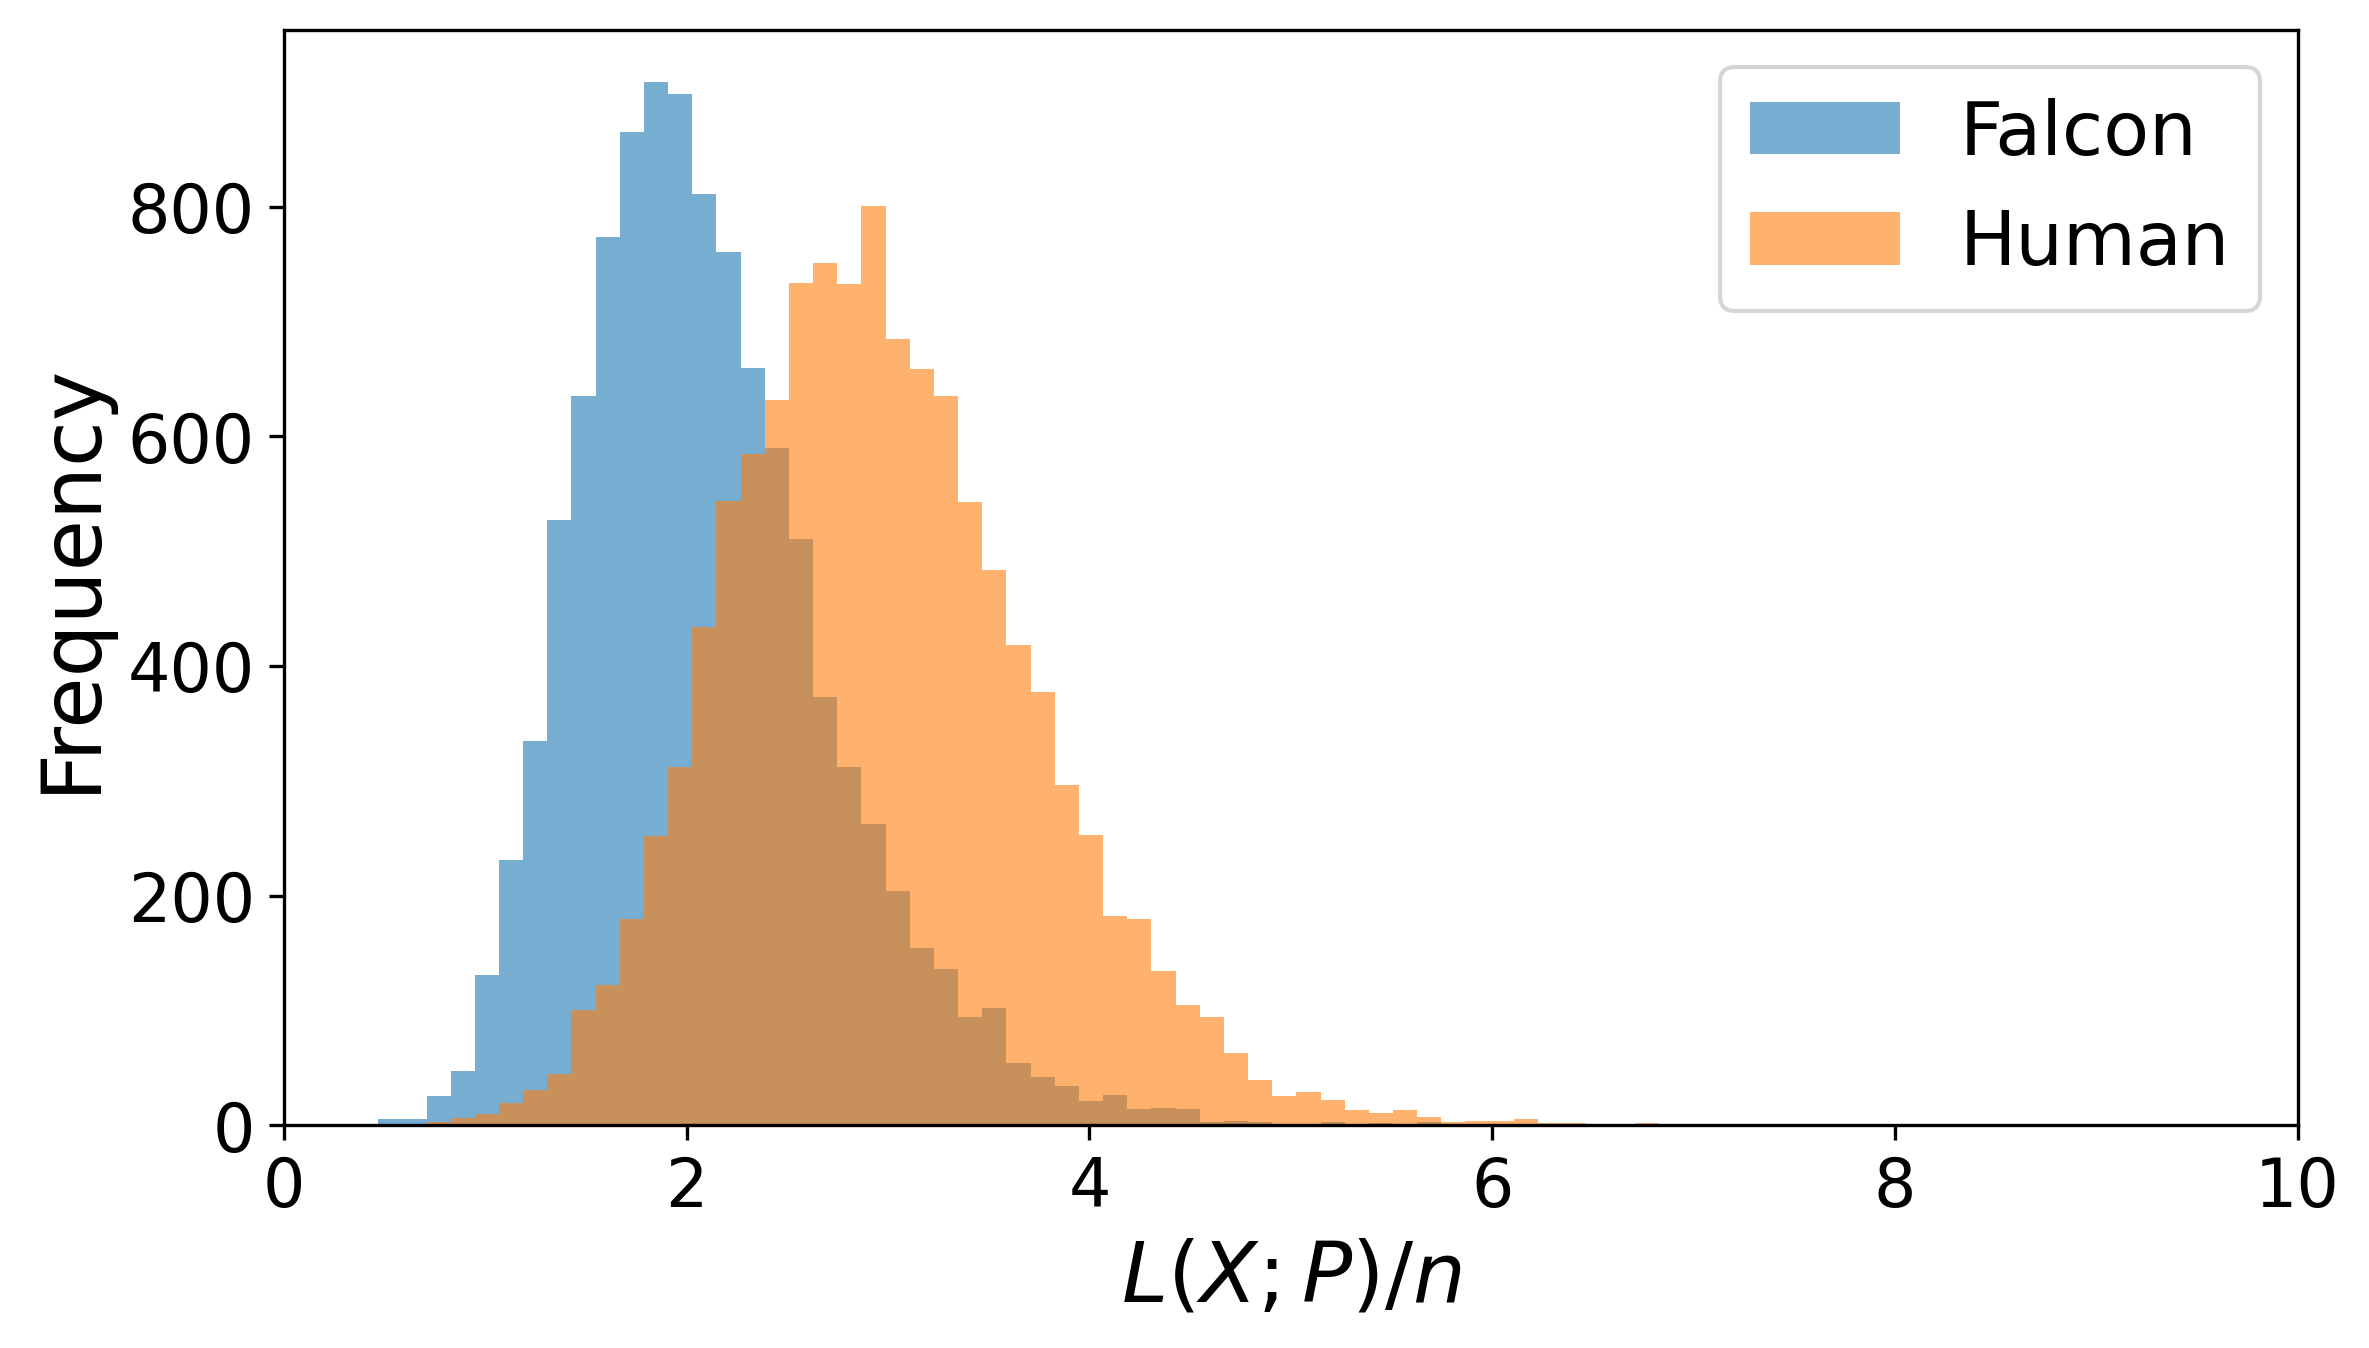
\includegraphics[width=\linewidth, height=0.57\textheight, keepaspectratio]
    {figures/presentation/response_hist_example_v2.png}

  \vspace{0.05em}
  {\scriptsize Related detectors: GLTR (Gehrmann et al., 2019),
   HowKGPT (Vasilatos et al., 2023), Binoculars (Hans et al., 2024).}

  \thesisline{The goal is maximum separation}
\end{frame}

% ------------------------------------------------------------------
% Frame 5 -- Related work
% ------------------------------------------------------------------
\begin{frame}{Related Work}
  \small
  \vfill
  Prior work addresses \textbf{adjacent problems} but not this
  \textbf{detector selection optimality question}:
  \vfill

  \begin{itemize}
    \setlength\itemsep{1.4em}

    \item \textbf{Unconstrained optimal detection} -
    Neyman-Pearson; Lehmann-Romano (2006)\\[-1pt]
    {\footnotesize When both models are known, thresholding the likelihood ratio
    \(\frac{G_1(X)}{G_0(X)}\) is optimal.}

    \item \textbf{Mismatched divergence} -
    Unnikrishnan, Huang, Meyn, Surana \& Veeravalli (2011)\\[-1pt]
    {\footnotesize Studies hypothesis testing when the ideal KL-based statistic
    is replaced by a mismatched one.}

    \item \textbf{M-projection / reverse I-projection} -
    Amari \& Nagaoka (2000)\\[-1pt]
    {\footnotesize Studies KL-based projection geometry over probability
    distributions; related to our objective, which is linear in
    \(\log p\).}

  \end{itemize}
  \vfill
\end{frame}

\note{
The oracle benchmark is Neyman-Pearson. Related work has studied
mismatched test statistics and KL projection geometry. Our work uses
this neighborhood of ideas, but applies it to choosing the detector model for
log-loss testing.
}

% ------------------------------------------------------------------
% Frame 6 -- Formal setup
% ------------------------------------------------------------------
\section{Setup}
\begin{frame}{Problem Setup}
  \begin{columns}[T,onlytextwidth]
    \begin{column}{0.60\textwidth}
      \textbf{Object:}\;
      \(X\) is the data sequence to attribute.

      \medskip
      \textbf{Hypothesis test:}
      \[
        H_0: X \sim G_0
        \qquad\text{vs.}\qquad
        H_1: X \sim G_1
      \]

      \textbf{Test statistic:}\;
      \(L(X;P) := \log \dfrac{1}{P(X)}\)

      \smallskip
      \textbf{Modeling assumption:}\; \(P\) lies near \(G_0\)
      {\small(shared tokenizer / architecture / training):}
      \[
        \boxed{P \in \cP_\epsilon(G_0)
               = \bigl\{P' : \Dkl{G_0}{P'} \leq \epsilon\bigr\}}
      \]

      {\small\textbf{Constrained optimality:}\; among detectors in this ball,
      we search for the one with maximum detection power.}
    \end{column}
    \hfill
    \begin{column}{0.36\textwidth}
      \centering
      \vspace{0.6em}
      \begin{tikzpicture}[scale=1.00]
        \shade[inner color=white, outer color=RUSoft]
              (0,0) circle (1.55cm);
        \draw[ultra thick, RUBlue] (0,0) circle (1.55cm);
        \node[RUBlue, font=\normalsize] at (0, 2.35)
             {\(\Dkl{G_0}{P}\!\leq\!\epsilon\)};
        \fill[RUBlue]   (0,0)      circle (2.5pt)
             node[below=5pt, font=\Large\bfseries]{\(G_0\)};
        \fill[orange!80!black] (2.55,1.3) circle (2.5pt)
             node[above right=-1pt, font=\large\bfseries]{\(G_1\)};
        \node[orange!80!black, font=\scriptsize, align=center] at (2.72,0.78)
             {alternative\\source};
        \fill[RUAccent] (0.65,0.82)  circle (2.5pt)
             node[right=3pt, font=\large\bfseries]{\(P\)};
        \fill[RUAccent] (-0.55,0.42) circle (2.5pt)
             node[left=3pt,  font=\large\bfseries]{\(P'\)};
        \fill[RUAccent] (0.35,-0.82) circle (2.5pt)
             node[right=3pt, font=\large\bfseries]{\(P''\)};
      \end{tikzpicture}
    \end{column}
  \end{columns}
\end{frame}

% ------------------------------------------------------------------
% Frame 7 -- Theorem 1: Delta controls power
% ------------------------------------------------------------------
\section{Main Result}
\begin{frame}{Result 1: Detector Power is Governed by \(\bigDelta\)}
  \small
  \textbf{Assumptions:} under \(G_0\) and \(G_1\), normalized log-loss is unimodal
  with variance stable across detectors.

  Power is monotone in the separation between the two log-loss distributions:
  \vspace{-0.25em}
  \[
    \mu_1(P)-\mu_0(P)
    =
    \underbrace{H(G_1)-H(G_0)}_{\text{fixed}}
    +
    \underbrace{\bigDelta(G_1,G_0;P)}_{\text{depends on }P}
  \]
  \vspace{-0.8em}
  {\Large
  \[
    \boxed{\bigDelta(G_1,G_0;P)
    :=\Dkl{G_1}{P}-\Dkl{G_0}{P}}
  \]
  }
  \vspace{-0.55em}

  \centering
  \begin{tikzpicture}[
      declare function={
        gauss(\x,\m,\s)=exp(-(\x-\m)^2/(2*\s^2))/(\s*sqrt(2*pi));
      }
    ]
    \begin{scope}[xscale=1.22, yscale=2.45]
      \draw[->, thick] (-3,0) -- (6.5,0)
           node[right, font=\footnotesize]{\(L(X;P)/n\)};
      \draw[RUBlue, very thick, domain=-3:3.8, samples=80]
           plot (\x, {gauss(\x,0,1)});
      \draw[red!70!black, very thick, domain=-0.8:6.5, samples=80]
           plot (\x, {gauss(\x,2.8,1)});
      \node[RUBlue, font=\small] at (0, 0.46)
           {\(\mu_0(P)\)};
      \node[red!70!black, font=\small] at (2.8, 0.46)
           {\(\mu_1(P)\)};
      \draw[<->, very thick, RUAccent]
           (0, -0.07) -- node[below, font=\small]
           {controlled by \(\bigDelta\)} (2.8, -0.07);
      \node[gray, font=\scriptsize, align=center] at (5.25, 0.32)
           {\(\sigma \approx\) stable\\[-1pt] across \(P\)};
    \end{scope}
  \end{tikzpicture}

  \vspace{-0.1em}
  \thesisline{Theorem~1: maximizing \(\bigDelta\) maximizes power at fixed Type-I level.}
\end{frame}

% ------------------------------------------------------------------
% Frame 8 -- Theorem 2: optimal detector for a simple alternative
% ------------------------------------------------------------------
\begin{frame}[t]{Result 2: Choosing the Optimal Detector \(P^*\)}
  \[
    \boxed{\vcenter{\hbox{$\displaystyle \max_{P \in \cP_\epsilon(G_0)}\;\bigDelta(G_1,G_0;P)$}}}
    \qquad\Longrightarrow\qquad
    \boxed{\vcenter{\hbox{$\displaystyle P^*(x)=G_0(x)-\gamma\bigl(G_1(x)-G_0(x)\bigr)$}}}
  \]
  \vspace{-0.3em}
  {\small\centering
  \textbf{Theorem 2:} \(P^*\) moves \alert{linearly away} from \(G_0\),
  opposite to \(G_1\), with \(D(G_0\|P^*)=\epsilon\).\par}

  \vspace{1.1em}
  \centering
  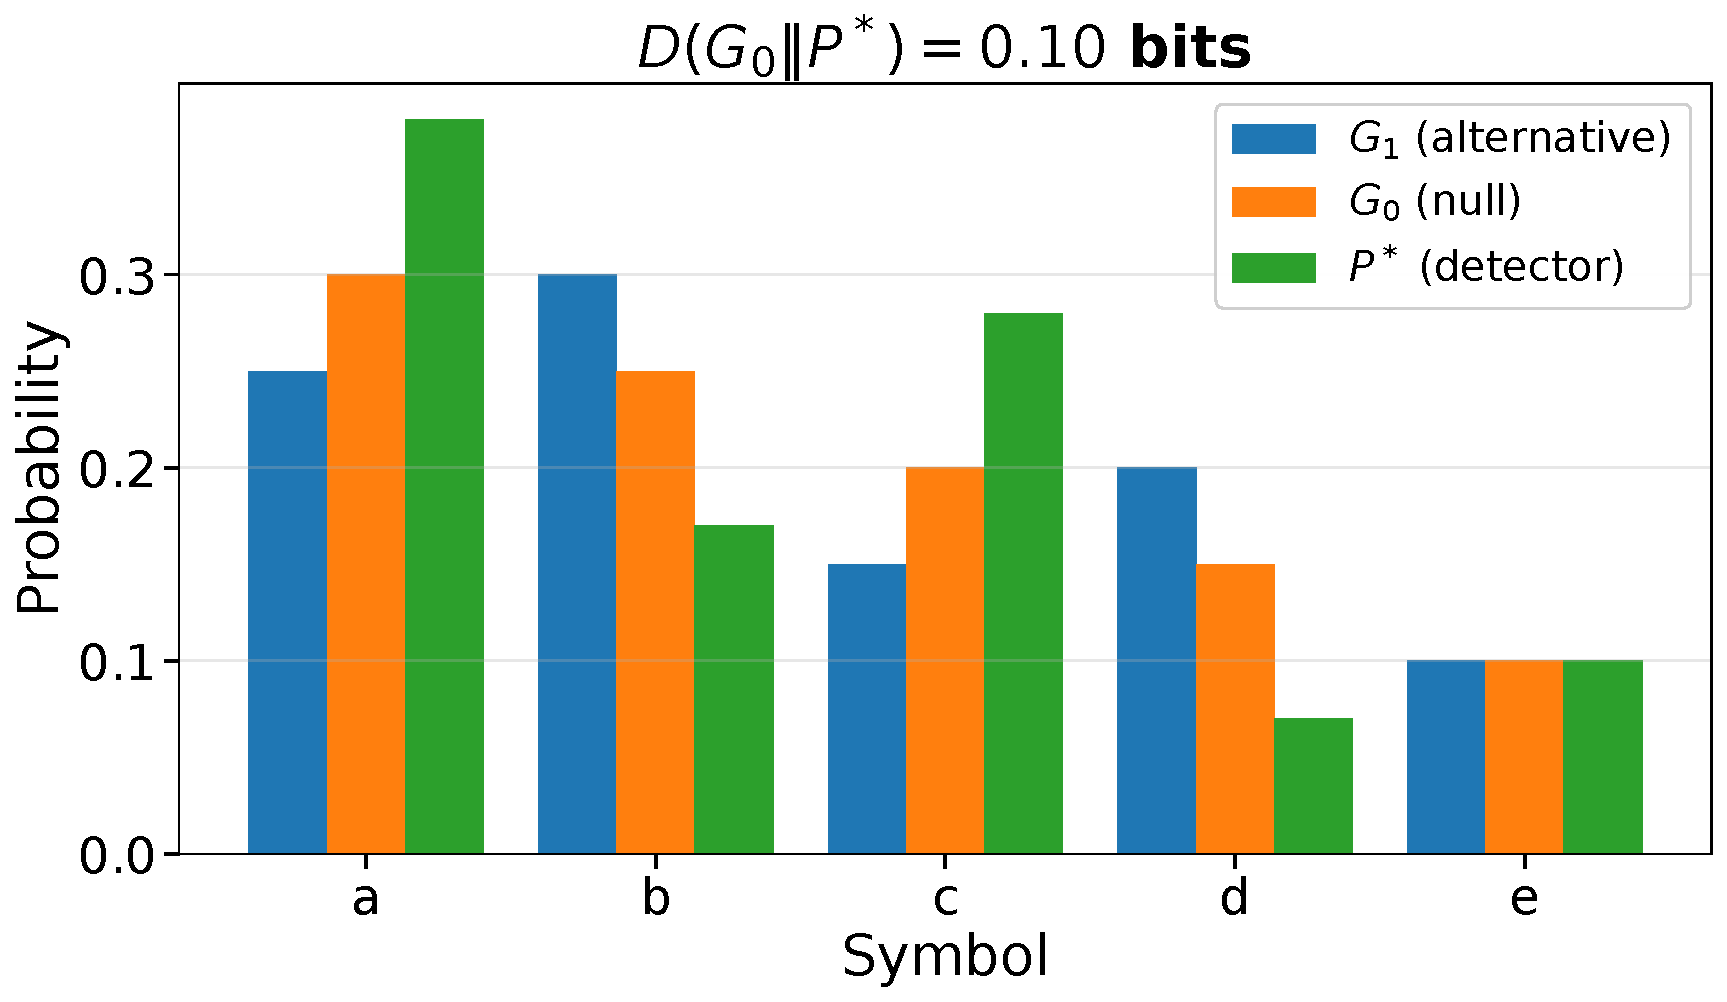
\includegraphics[width=0.80\linewidth, height=0.605\textheight, keepaspectratio]
    {figures/presentation/epsilon_ball_example.pdf}
\end{frame}

\note{
\textbf{Geometry of $P^*$ (Theorem 2).}
\begin{itemize}\small
  \item \textbf{The space is the probability simplex}: $G_0$, $G_1$, $P^*$ are
        each one point = a distribution over the alphabet. $G_1-G_0$ is the
        direction from $G_0$ toward $G_1$; $P^*$ steps the \emph{opposite} way
        (away from $G_1$) along a straight line.
  \item \textbf{Linear}, not geometric/exponential --- the small surprise of
        Thm~2. It subtracts mass from tokens where $G_1$ dominates, raising
        $-\log P$ there.
  \item $\epsilon$ = radius of the KL ball (the budget we choose); in the
        figure $\epsilon = 0.10$ bits --- that is exactly the
        ``$D(G_0\|P^*)=0.10$ bits'' label.
  \item $\gamma$ = step size in the formula; it is NOT free. Eq.~(10),
        $D(G_0\|P^*)=\epsilon$, pins $\gamma$ so $P^*$ lands exactly on the
        ball's boundary (constraint active, since $\Delta$ grows as we move
        away from $G_0$). So $\epsilon$ isn't written in eq.~(9): it enters
        through $\gamma$. Bigger $\epsilon\Rightarrow$ bigger
        $\gamma\Rightarrow P^*$ farther from $G_0$.
  \item \textbf{$\gamma\Leftrightarrow\epsilon$ relation:} no closed form in general
        (solve $\epsilon=-\sum_x G_0\log(1-\gamma\tfrac{G_1-G_0}{G_0})$,
        monotone in $\gamma$). Small-$\epsilon$:
        $\gamma\approx\sqrt{2\epsilon/\Dchi{G_1}{G_0}}$, i.e.
        $\gamma\propto\sqrt\epsilon$. This is the engine behind the
        Thm~3 gain $\sqrt{2\epsilon\,\Dchi{G_1}{G_0}}$.
        ($\epsilon$ in nats; $1/\ln2$ factor if in bits.)
\end{itemize}
}

% ------------------------------------------------------------------
% Frame 9 -- Composite alternatives and self-detection
% ------------------------------------------------------------------
\section{Composite Alternatives}
\begin{frame}[t]{Result 3: When Self-Detection is Locally Maximin-Optimal}
  \vspace{1.2em}
  \begin{columns}[c,onlytextwidth]
    \begin{column}{0.60\textwidth}
      {\small
      \textbf{Single \(G_1\):} move away from \(G_0\).\\[0.25em]
      \textbf{Family of alternatives \(\cG_1\):} optimize the worst case.}

      \[
        \bigDelta^*(\cG_1,G_0)=
        \sup_{P\in\cP_\epsilon(G_0)}\inf_{G\in\cG_1}\bigDelta(G,G_0;P)
      \]

      \vspace{0.5em}
      {\small \textbf{Modeling assumption:} LLM \(G_0\) can be viewed as a learned
      convex mixture of human-style sources:}

      \[
        G_0 \approx \sum_j \pi_j H_j
        \qquad \text{\footnotesize\(\pi_j\ge 0,\ \sum\nolimits_j \pi_j=1\)}
      \]
    \end{column}
    \hfill
    \begin{column}{0.39\textwidth}
      \centering
      \begin{tikzpicture}[scale=1.08]
        \fill[RUBlue] (0,0) circle (3pt)
             node[below=5pt, font=\normalsize]{$G_0$ {\footnotesize(LLM)}};
        \foreach \a in {0,20,...,340} {
          \pgfmathsetmacro{\r}{1.4+0.18*rand}
          \fill[red!50!black, opacity=0.55] (\a:\r) circle (1.8pt);
        }
        \draw[dashed, RUAccent, thick] (0,0) circle (1.6cm);
        \node[black, font=\small, align=center] at (0, -2.35)
             {alternative sources\\[-1pt] around \(G_0\)};
      \end{tikzpicture}
    \end{column}
  \end{columns}

  \vspace{0.15em}
  \begin{callout}[width=0.92\linewidth]
    {\small If alternatives \alert{isotropically surround} \(G_0\):}\\[2pt]
    {\Large \(\boldsymbol{P=G_0}\) is locally maximin optimal}
  \end{callout}
\end{frame}

% ------------------------------------------------------------------
% Frame 10 -- Empirical: normalized log-loss separation predicts AUC
% ------------------------------------------------------------------
\section{Evidence}
\begin{frame}[t]{Empirical Check: Normalized Separation Predicts AUC}
  \begin{columns}[c,onlytextwidth]
    \begin{column}{0.73\textwidth}
      \centering
      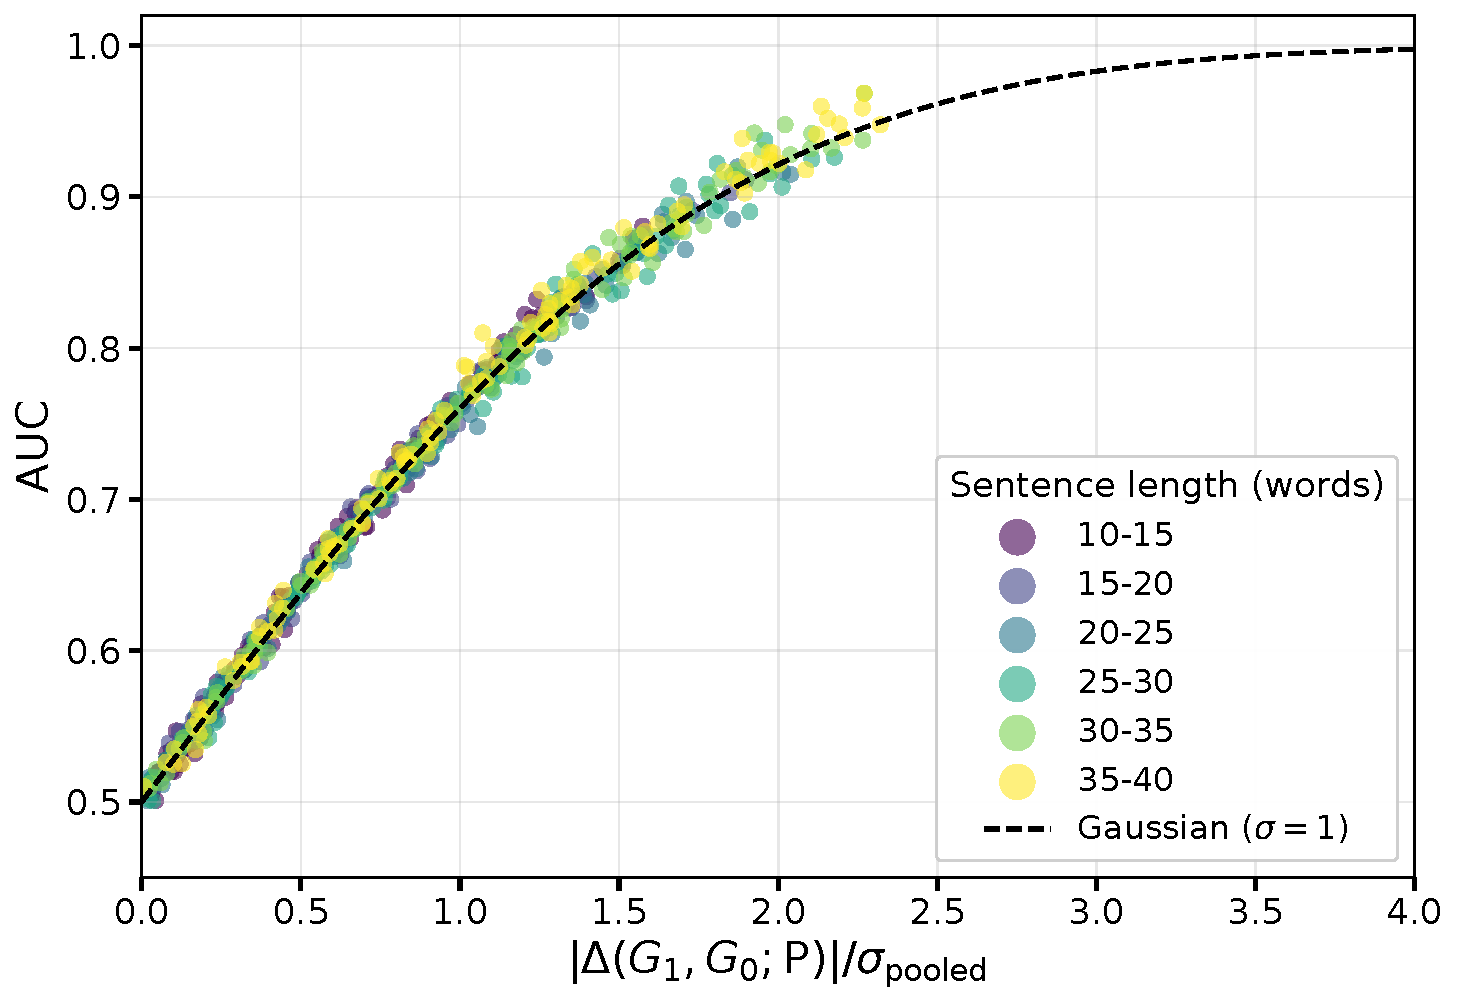
\includegraphics[width=\linewidth, height=0.625\textheight, keepaspectratio]
        {figures/presentation/auc_vs_delta_normalized_unified.pdf}
    \end{column}
    \hfill
    \begin{column}{0.25\textwidth}
      \small\textcolor{black!78}{%
      \(\displaystyle x:=\frac{|\hat\mu_1(P)-\hat\mu_0(P)|}{\hat\sigma_{\mathrm{pooled}}}\)\\[12pt]
      \(\mathrm{AUC}\approx\Phi(x/\sqrt{2})\)}
    \end{column}
  \end{columns}

  \vspace{0.3em}
  {\small \textbf{Experiment setup:} 275,000 sentences, 3 domains, 5 authors, 4 detector models}\\[2pt]
  {\small Empirical AUC follows the Gaussian curve:
  \alert{Pearson \(r=0.99\).}}\\[2pt]
  {\small\textcolor{RUBlue}{\textbf{Supports Result 1:}
  Gaussian-like log-loss behavior and stable variance.}}\\[2pt]
  {\footnotesize\textcolor{black!78}{Max/min standard-deviation ratio
  across detectors is \(1.2\)--\(1.5\times\).}}
\end{frame}

\note{
\textbf{VALIDATION, not a discovery.}
\begin{itemize}\small
  \item Don't pitch ``more separation $\to$ higher AUC'' as a finding ---
        obvious/monotone for any score.
  \item $\Phi(x/\sqrt2)$ = textbook binormal-AUC formula
        ($\mathrm{AUC}=\Pr(S_1>S_0)$ for two equal-variance Gaussians).
        We did NOT compute AUC with it: AUC is measured from the ROC
        (\texttt{roc\_auc\_score}); the curve is just overlaid. Parameter-free.
  \item Three claims tested: (1) $\Delta=D(G_1\|P)-D(G_0\|P)$ governs separation
        (Thm~1, not a priori obvious); (2) the unimodal, variance-stable
        Gaussian model (A1--A2) holds on real text; (3) the link is
        quantitative, not just directional.
  \item $r=0.99$ supports \textbf{A1--A2} (paper attributes Fig.~3 to A1--A2).
        \textbf{A3} ($\sigma$ independent of $P$) is checked \emph{separately}
        by the $1.2$--$1.5\times$ $\sigma$-ratio (Fig.~2). Single-$\sigma$ form
        assumes $\sigma_0\approx\sigma_1$; else
        $\Phi\!\big((\mu_1-\mu_0)/\sqrt{\sigma_0^2+\sigma_1^2}\big)$.
  \item Say: ``AUC measured from the ROC follows the parameter-free $\Phi(x/\sqrt2)$
        almost perfectly, so Thm~1's assumptions hold.'' Contribution = THEORY
        ($\Delta$ governs power; $P=G_0$ can be maximin); plot = credibility check.
\end{itemize}
}

% ------------------------------------------------------------------
% Frame 11 -- Human vs LLM evidence
% ------------------------------------------------------------------
\begin{frame}[t]{LLM vs.\ Human: Support for the Maximin Choice \(P=G_0\)}
  \centering
  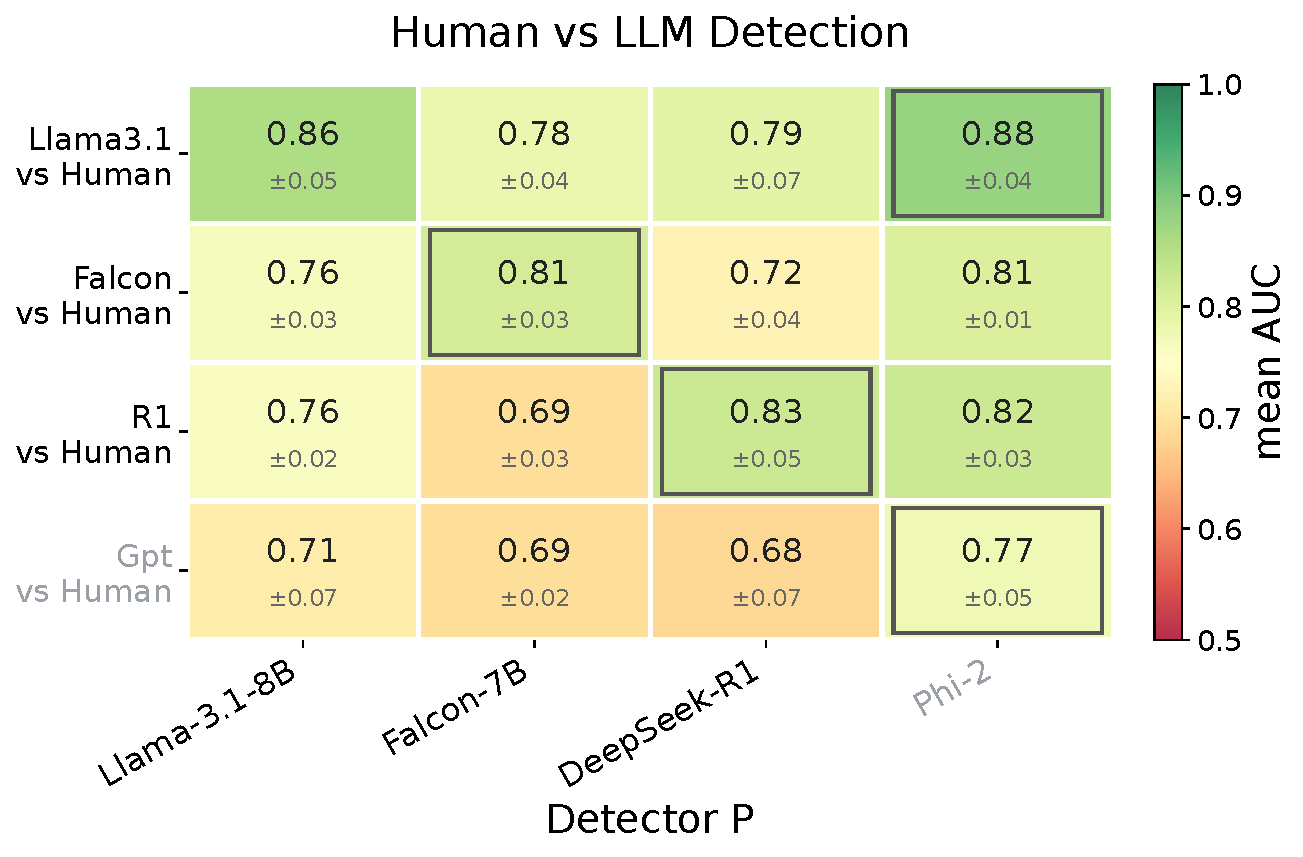
\includegraphics[width=0.98\linewidth, height=0.63\textheight, keepaspectratio]
    {figures/presentation/human_detection_heatmap_avg.pdf}

  \vfill
  \begin{columns}[c,onlytextwidth]
    \begin{column}{0.42\textwidth}
      \small\textbf{Matched detector \(P=G_0\):}
      \begin{itemize}
        \setlength\itemsep{0.1em}
        \item \alert{Best in 4/9} cases, second-best in 5/9
        \item Mean AUC \(\mathbf{0.831}\) vs.\ \(0.626\) for LLM-vs-LLM
      \end{itemize}
    \end{column}
    \hfill
    \begin{column}{0.55\textwidth}
      \begin{callout}[top=4pt,bottom=4pt,before skip=0pt,after skip=0pt,
          colframe=RUBlue!45, boxrule=0.5pt,
          borderline west={3pt}{0pt}{RUAccent}]
        \small Consistent with the maximin model if LLM \(G_0\) is surrounded
        by human sources.
      \end{callout}
    \end{column}
  \end{columns}
\end{frame}

% ------------------------------------------------------------------
% Frame 12 -- Contribution, not recap
% ------------------------------------------------------------------
\section{Takeaway}
\begin{frame}{Takeaway}
  \vfill
  \begin{enumerate}
    \setlength{\itemsep}{2.6em}
    \item When candidate-model likelihoods are unavailable,
          detect with a third model \(P\).

    \item The power-maximizing detector maximizes
          \(\bigDelta(G_1,G_0;P)=\Dkl{G_1}{P}-\Dkl{G_0}{P}\).

    \item For composite alternatives isotropically surrounding \(G_0\),
          self-detection is locally the maximin optimal choice.
  \end{enumerate}
  \vfill
\end{frame}

% ------------------------------------------------------------------
% Frame 13 -- Landing
% ------------------------------------------------------------------
{
\setbeamercolor{background canvas}{bg=RUBlue}
\setbeamercolor{normal text}{fg=white}
\usebeamercolor[fg]{normal text}
\hypersetup{urlcolor=white}
\begin{frame}[plain, c]
  \centering
  {\LARGE\textbf{Choose the detector. Maximize the gap.}}\\[1.8em]
  {\normalsize
    Adam Vinestock \quad\textbullet\quad
    \href{mailto:adam.vinestock@post.runi.ac.il}%
         {\texttt{adam.vinestock@post.runi.ac.il}}\\[3pt]
    Alon Kipnis \quad\textbullet\quad
    \href{mailto:alon.kipnis@runi.ac.il}%
         {\texttt{alon.kipnis@runi.ac.il}}
  }\\[1.4em]
  {\small Extended version \& proofs}\\[2pt]
  {\footnotesize\href{https://cs.idc.ac.il/~kipnis}%
                     {\texttt{cs.idc.ac.il/\~{}kipnis}}}
\end{frame}
}

% =================================================================
% BACKUP / APPENDIX
% =================================================================
\appendix
\metroset{numbering=none, progressbar=none}

% ------------------------------------------------------------------
% Backup B1 -- Theorem 3
% ------------------------------------------------------------------
\begin{frame}{How Sub-Optimal Is \(P=G_0\)?}
  Small-\(\epsilon\) expansion of the optimal gap:
  \[
    \bigDelta(G_1,G_0;P^*)
    =
    \Dkl{G_1}{G_0}
    +\sqrt{2\epsilon\,\Dchi{G_1}{G_0}}
    +O(\epsilon).
  \]

  \medskip
  \begin{callout}
    Deviating from \(G_0\) can raise the gap by
    \(\approx\sqrt{2\epsilon\,\Dchi{G_1}{G_0}}\),
    quantifying the sub-optimality of \(P=G_0\) against a
    \textbf{simple} alternative.
  \end{callout}

  \medskip
  \textbf{Where this comes from: the \(\gamma \Leftrightarrow \epsilon\) relation.}
  The constraint \(D(G_0\|P^*)=\epsilon\) fixes the step size \(\gamma\).
  It has no closed form in general, but for small \(\epsilon\)
  \[
    \epsilon \approx \tfrac{\gamma^2}{2}\,\Dchi{G_1}{G_0}
    \qquad\Longleftrightarrow\qquad
    \gamma \approx \sqrt{\tfrac{2\epsilon}{\Dchi{G_1}{G_0}}}
    \;\;(\gamma\propto\sqrt{\epsilon}),
  \]
  which substituted into the gap produces the
  \(\sqrt{2\epsilon\,\Dchi{G_1}{G_0}}\) term above.

  \medskip
  {\footnotesize Here
  \(\Dchi{G_1}{G_0}=\sum_x (G_1(x)-G_0(x))^2/G_0(x)\);
  \(\epsilon\) in nats (\(1/\ln2\) factor if measured in bits).}
\end{frame}

% ------------------------------------------------------------------
% Backup B2 -- Theorem 4
% ------------------------------------------------------------------
\begin{frame}{The Maximin Mechanism}
  For a composite family \(\cG_1\), the local maximin gap is set by
  a least-favorable prior \(\pi^*\):
  \[
    \bigDelta^*(\cG_1,G_0)
    =
    \mathbb{E}_{G\sim\pi^*}\!\left[\Dkl{G}{G_0}\right]
    +\sqrt{2\epsilon\,\Dchi{\bar G_{\pi^*}}{G_0}}
    +O(\epsilon),
  \]
  \[
    \bar G_{\pi^*}(x)=\mathbb{E}_{G\sim\pi^*}[G(x)].
  \]

  \begin{callout}
    If a non-convex alternative family isotropically surrounds \(G_0\),
    this mechanism yields Corollary 5.1: \(P=G_0\) is locally maximin.
  \end{callout}
\end{frame}

% ------------------------------------------------------------------
% Backup B2b -- Anisotropy index detail (definitions pushed off main slide 8)
% ------------------------------------------------------------------
\begin{frame}{Anisotropy Index and Isotropic Optimality}
  For a prior \(\pi^{\#}\) on \(\cG_1\) with \(G_0=\bar G_{\pi^{\#}}=\mathbb{E}_{G\sim\pi^{\#}}[G]\):
  \[
    \bar D_{\pi^{\#}}=\mathbb{E}_{G\sim\pi^{\#}}\Dkl{G}{G_0},
    \qquad
    r_{\pi^{\#}}=\sup_{G\in\operatorname{supp}(\pi^{\#})}
      \bigl|\Dkl{G}{G_0}-\bar D_{\pi^{\#}}\bigr|.
  \]
  \(r_{\pi^{\#}}=0\) iff all sources are equidistant from \(G_0\) in relative
  entropy (the mixture is isotropic); it grows with the unevenness of those
  distances.

  \medskip
  For any alternative \(G\in\cG_1\), the self-detector \(P=G_0\) obeys
  \[
    \bigDelta(G,G_0;G_0)=\Dkl{G}{G_0}
    \;\ge\;\bigDelta^*(\cG_1,G_0)-r_{\pi^{\#}}+O(\epsilon),
  \]
  so its worst-case sub-optimality is at most \(r_{\pi^{\#}}\). When
  \(r_{\pi^{\#}}=0\),
  \[
    \inf_{G\in\cG_1}\Dkl{G}{G_0}=\bigDelta^*(\cG_1,G_0)+O(\epsilon),
  \]
  i.e.\ \(P=G_0\) is locally maximin optimal.
\end{frame}

% ------------------------------------------------------------------
% Backup B3 -- Experimental setup
% ------------------------------------------------------------------
\begin{frame}{Experimental Setup}
  \begin{columns}[T,onlytextwidth]
    \begin{column}{0.48\textwidth}
      \textbf{Datasets} {\small(3 domains, matched topics)}
      \begin{itemize}
        \setlength\itemsep{0.25em}
        \item Wikipedia, News, Scientific abstracts
        \item \(\sim\!4{,}500\) docs, \(\sim\!275{,}000\) sentences
        \item Sentence length: 10--40 words
        \item Scored without preceding context
      \end{itemize}
    \end{column}
    \hfill
    \begin{column}{0.48\textwidth}
      \textbf{Authors / Detectors}
      \begin{itemize}
        \setlength\itemsep{0.25em}
        \item Authors: Llama-3.1, Falcon, GPT-3.5, DeepSeek-R1, Human
        \item Detectors \(P\): Llama-3.1, Falcon, Phi-2, DeepSeek-R1
        \item Some coincide \(\Rightarrow\) self-detection (\(P=G_0\))
      \end{itemize}
    \end{column}
  \end{columns}

  \vfill
  \begin{callout}
    GPT-3.5 model inaccessible for evaluation, so self-detection
    isn't possible.
  \end{callout}
\end{frame}

% ------------------------------------------------------------------
% Backup B4 -- Length confounding
% ------------------------------------------------------------------
\begin{frame}{Why Normalize?}
  \centering
  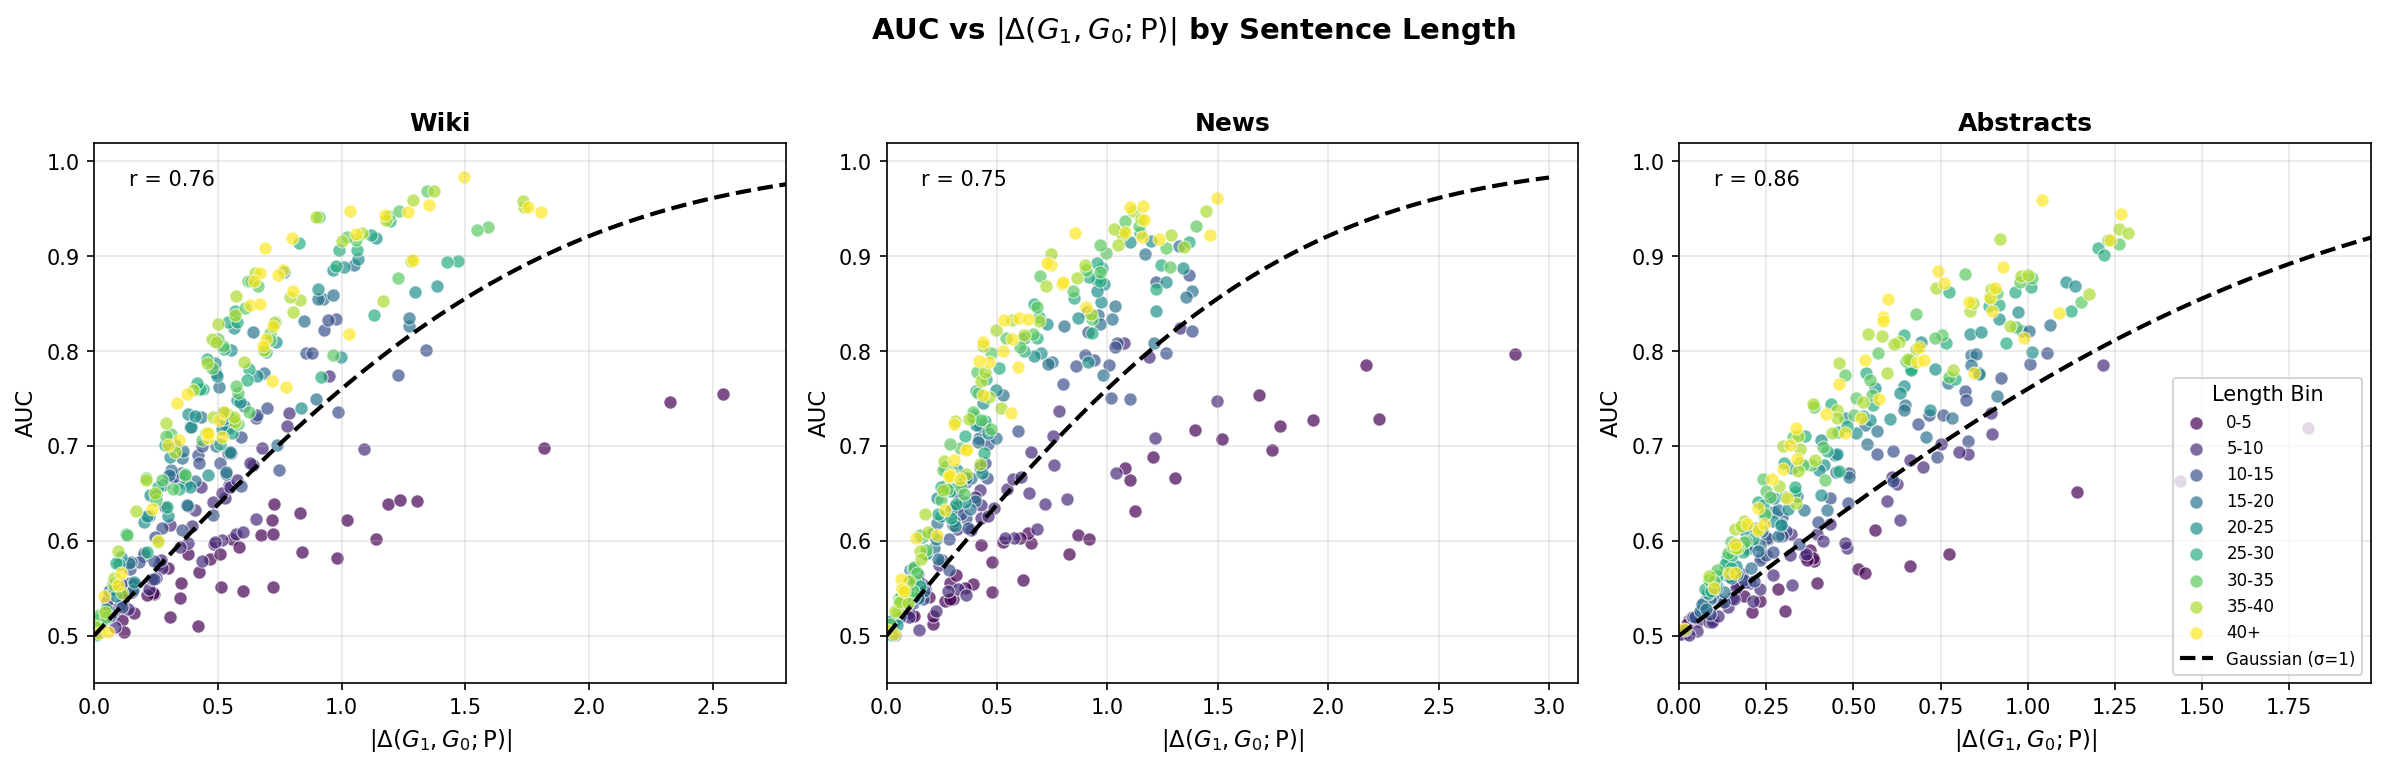
\includegraphics[width=0.95\linewidth, height=0.66\textheight, keepaspectratio]
    {figures/delta_auc_by_length.png}

  \vspace{0.3em}
  {\small Raw log-loss gaps are confounded by length. Dividing by
  \(\hat\sigma_{\mathrm{pooled}}\) collapses length bins onto the
  Gaussian AUC curve used in the main evidence slide.}
\end{frame}

% ------------------------------------------------------------------
% Backup B5 -- Variance stability
% ------------------------------------------------------------------
\begin{frame}{Variance Stability by Length}
  \centering
  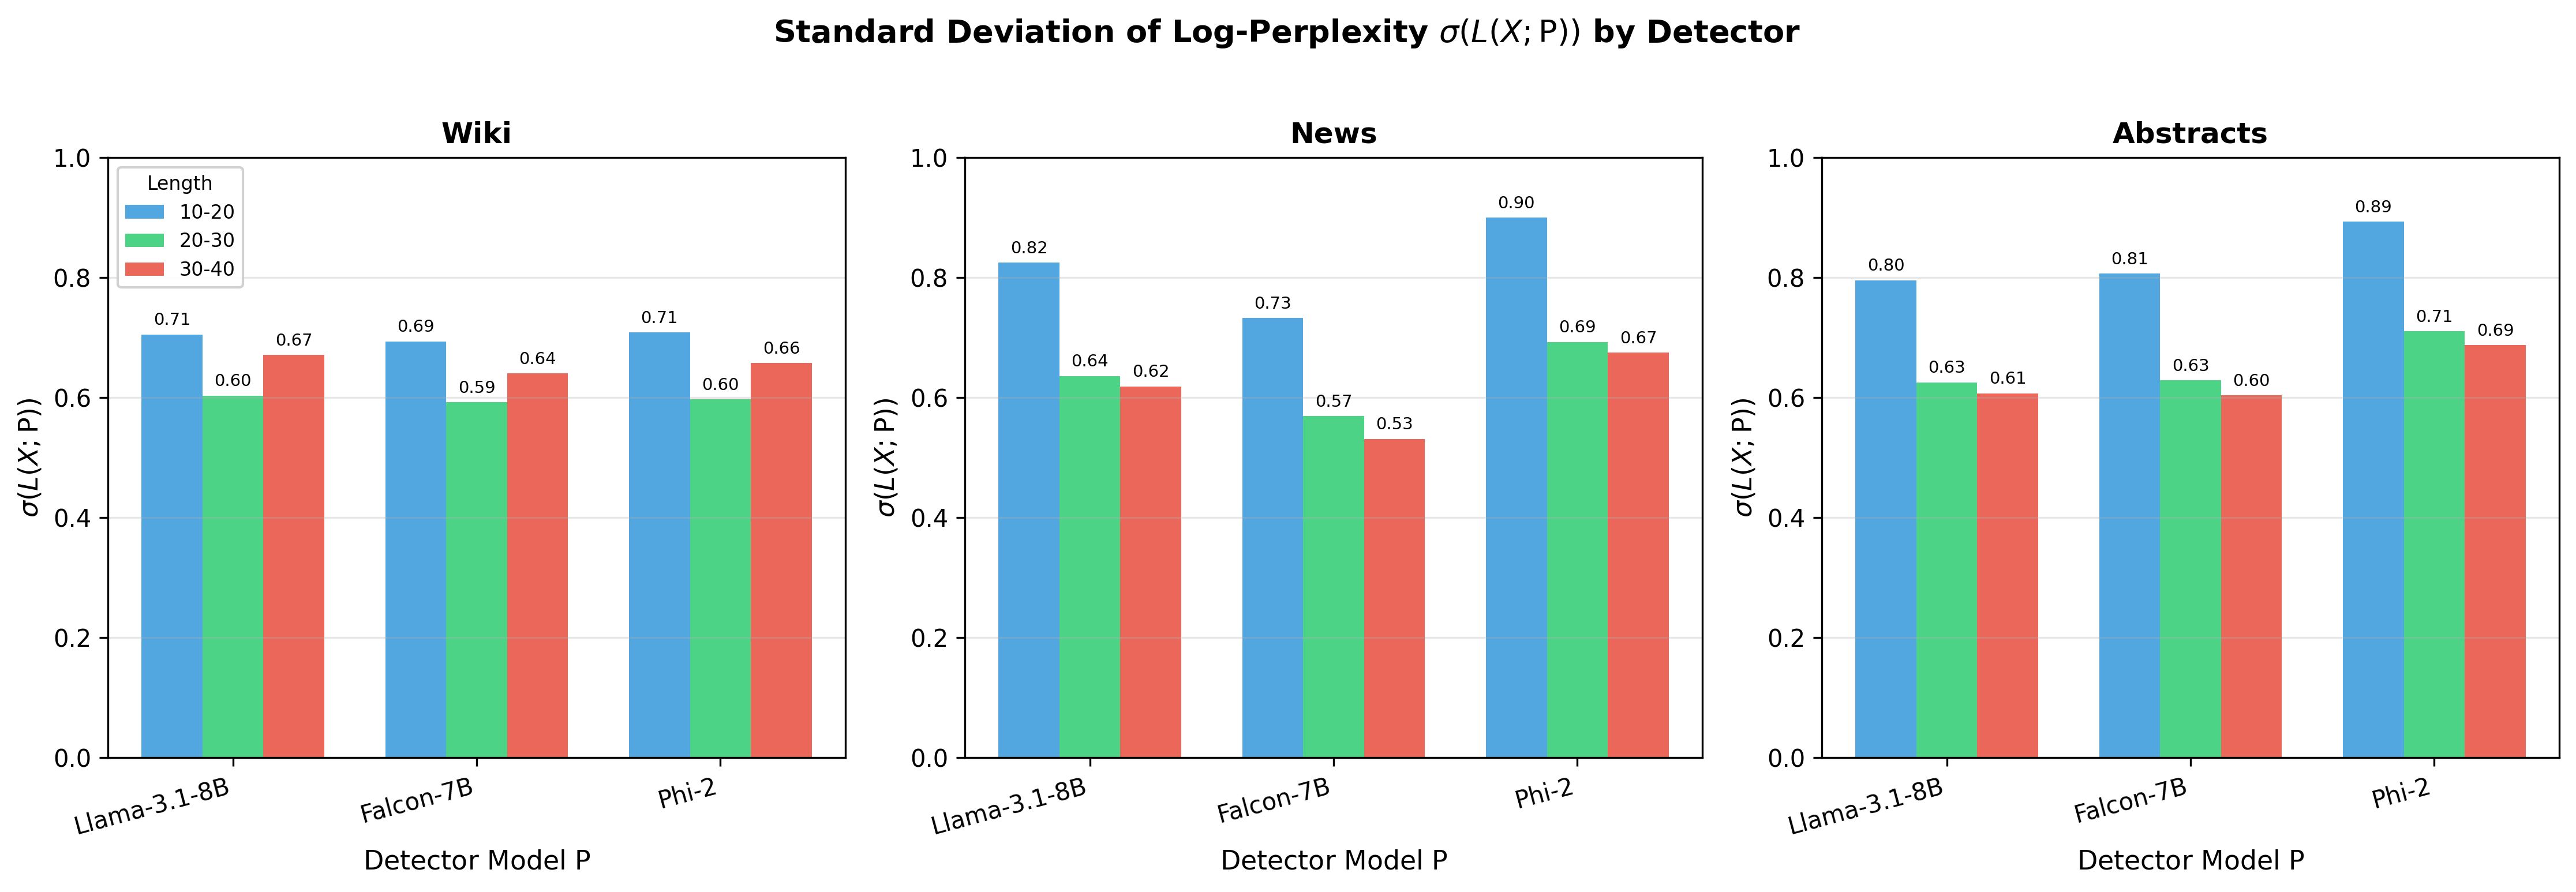
\includegraphics[width=\linewidth, height=0.62\textheight, keepaspectratio]
    {figures/sigma_vs_detector.png}

  \vspace{0.3em}
  {\small A3 view: standard deviation \(\sigma(L(X;P))\) by detector, split by
  sentence length. \emph{Within each length bin}, \(\sigma\) is nearly identical
  across Llama-3.1, Falcon, and Phi-2 (across-detector ratio \(\approx
  1.0\)--\(1.3\times\)), supporting A3; the larger spread within a dataset is
  driven by length, not by \(P\). DeepSeek-R1 is excluded as an outlier (its
  chat template inflates \(\sigma\)).}
\end{frame}

% ------------------------------------------------------------------
% Backup B6 -- Matched-detector counting
% ------------------------------------------------------------------
\begin{frame}{What ``Best in 4/9'' Means}
  \begin{itemize}
    \setlength\itemsep{0.55em}
    \item \textbf{The 9 cases:} 3 domains \(\times\) 3 matched LLM authors
          (Llama-3.1, Falcon, DeepSeek-R1).
    \item \textbf{GPT is excluded:} it has no corresponding open detector.
    \item \textbf{Phi-2 is detector-only:} it can win a heatmap cell, but
          is not part of the matched-detector count.
    \item \textbf{The claim:} among matched-detector cases,
          \(P=G_0\) is best in 4/9 and second-best in the remaining 5/9.
  \end{itemize}
\end{frame}

% ------------------------------------------------------------------
% Backup B7 -- AUC table
% ------------------------------------------------------------------
\begin{frame}{Matched-Detector AUC Numbers}
  \vfill
  \centering
  \textbf{AUC when detector matches source (\(P=G_0\))}

  \vspace{0.8em}
  \begin{tabular}{@{}lccc@{}}
    \toprule
    Dataset & Human vs.\ \(G_0\) & \(G_0\) vs.\ \(G_1\) & Gap \\
    \midrule
    Wiki      & \(0.853 \pm 0.006\) & \(0.659 \pm 0.065\) & \(+0.194\) \\
    News      & \(0.854 \pm 0.047\) & \(0.626 \pm 0.094\) & \(+0.229\) \\
    Abstracts & \(0.787 \pm 0.018\) & \(0.592 \pm 0.013\) & \(+0.195\) \\
    \midrule
    \textbf{Mean} & \(\mathbf{0.831}\) & \(\mathbf{0.626}\)
                  & \(\mathbf{+0.206}\) \\
    \bottomrule
  \end{tabular}

  \vspace{0.8em}
  {\small Human-vs-LLM self-detection is substantially easier than
  LLM-vs-LLM matched detection in this experiment.}
  \vfill
\end{frame}

% ------------------------------------------------------------------
% Backup B8--B10 -- Original (paper) versions of the updated plots
% ------------------------------------------------------------------
\begin{frame}{Backup: Original \(P^*\) Example (paper figure)}
  \centering
  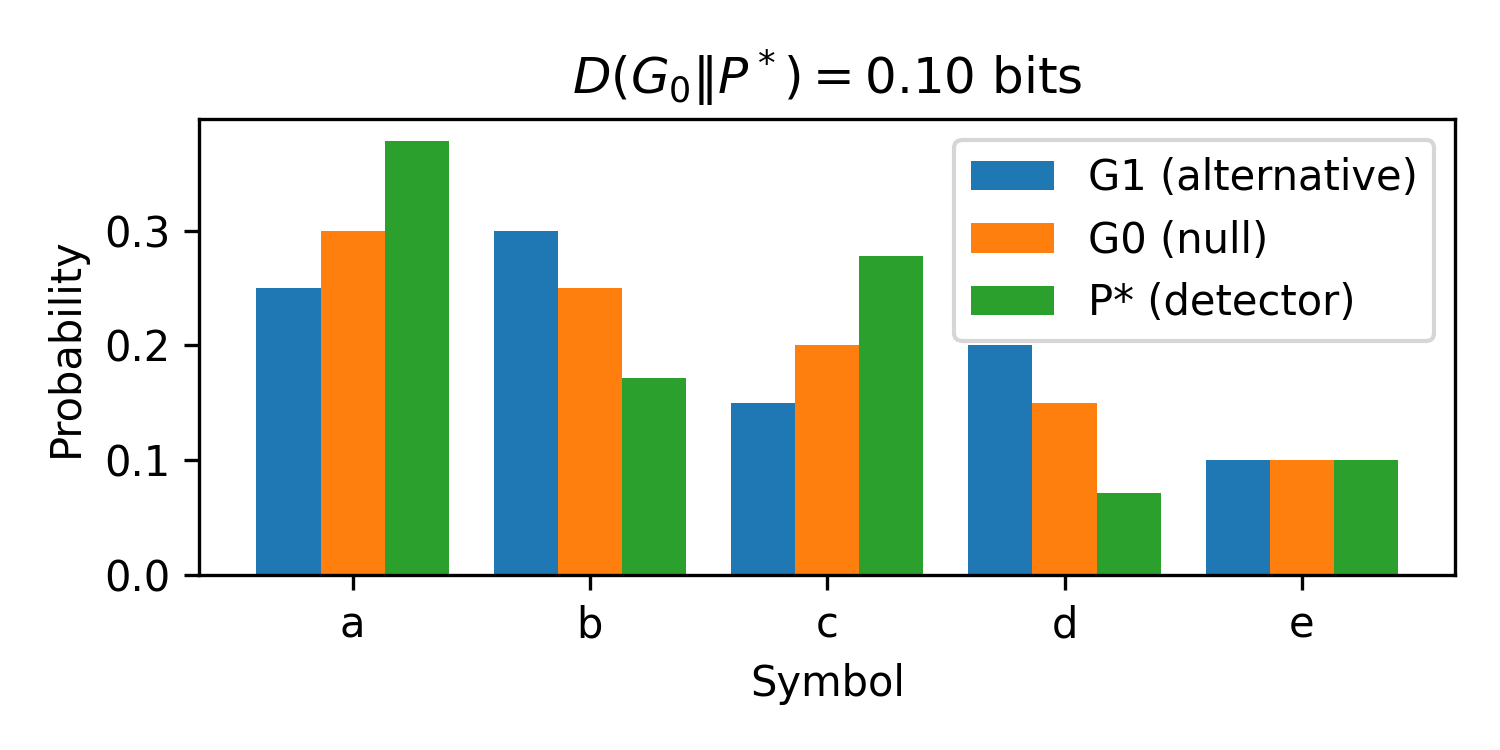
\includegraphics[width=0.92\linewidth, height=0.74\textheight, keepaspectratio]
    {figures/epsilon_ball_example.png}
\end{frame}

\begin{frame}{Backup: Original AUC vs Normalized Separation (paper figure)}
  \centering
  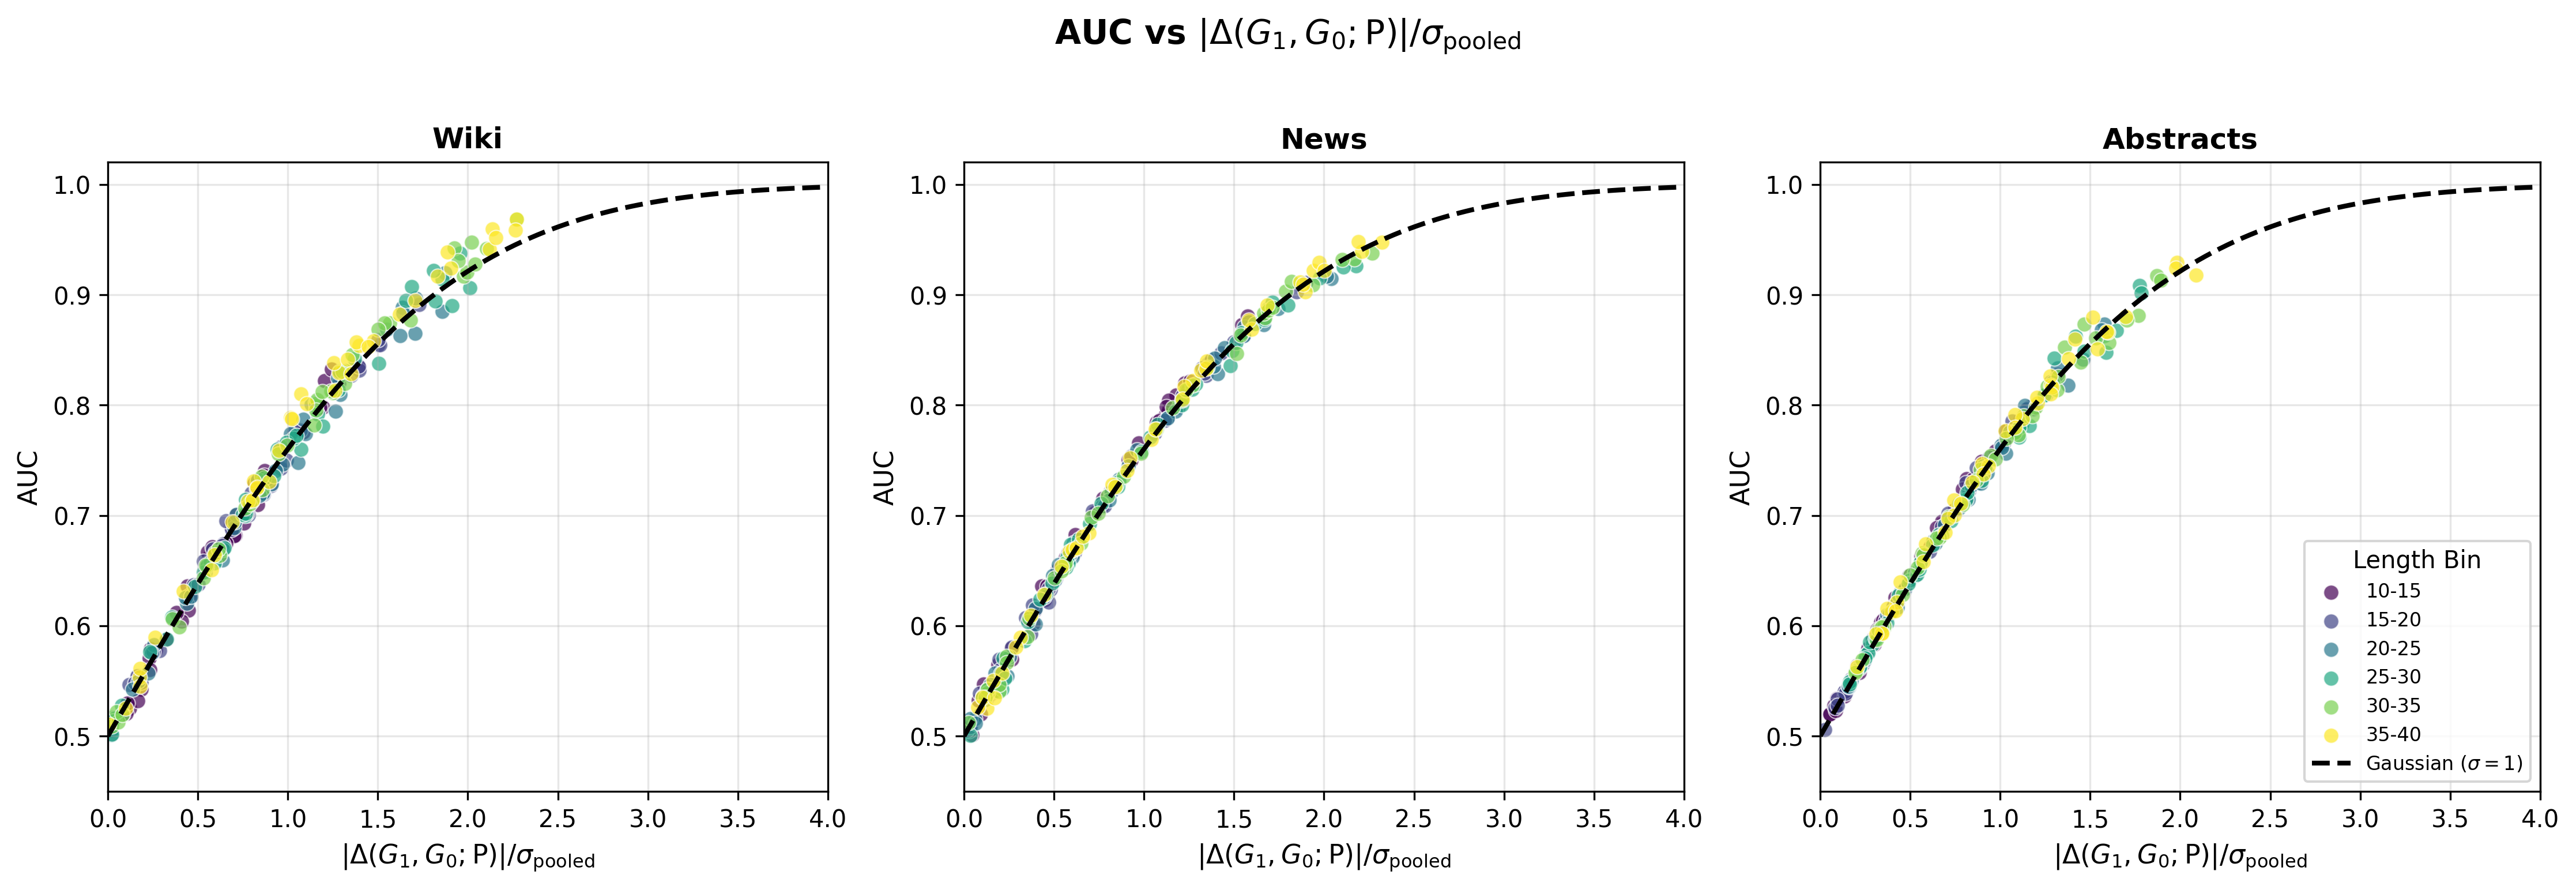
\includegraphics[width=0.96\linewidth, height=0.78\textheight, keepaspectratio]
    {figures/auc_vs_delta_normalized.png}
\end{frame}

\begin{frame}{Backup: Original Human-vs-LLM Heatmap (paper figure)}
  \centering
  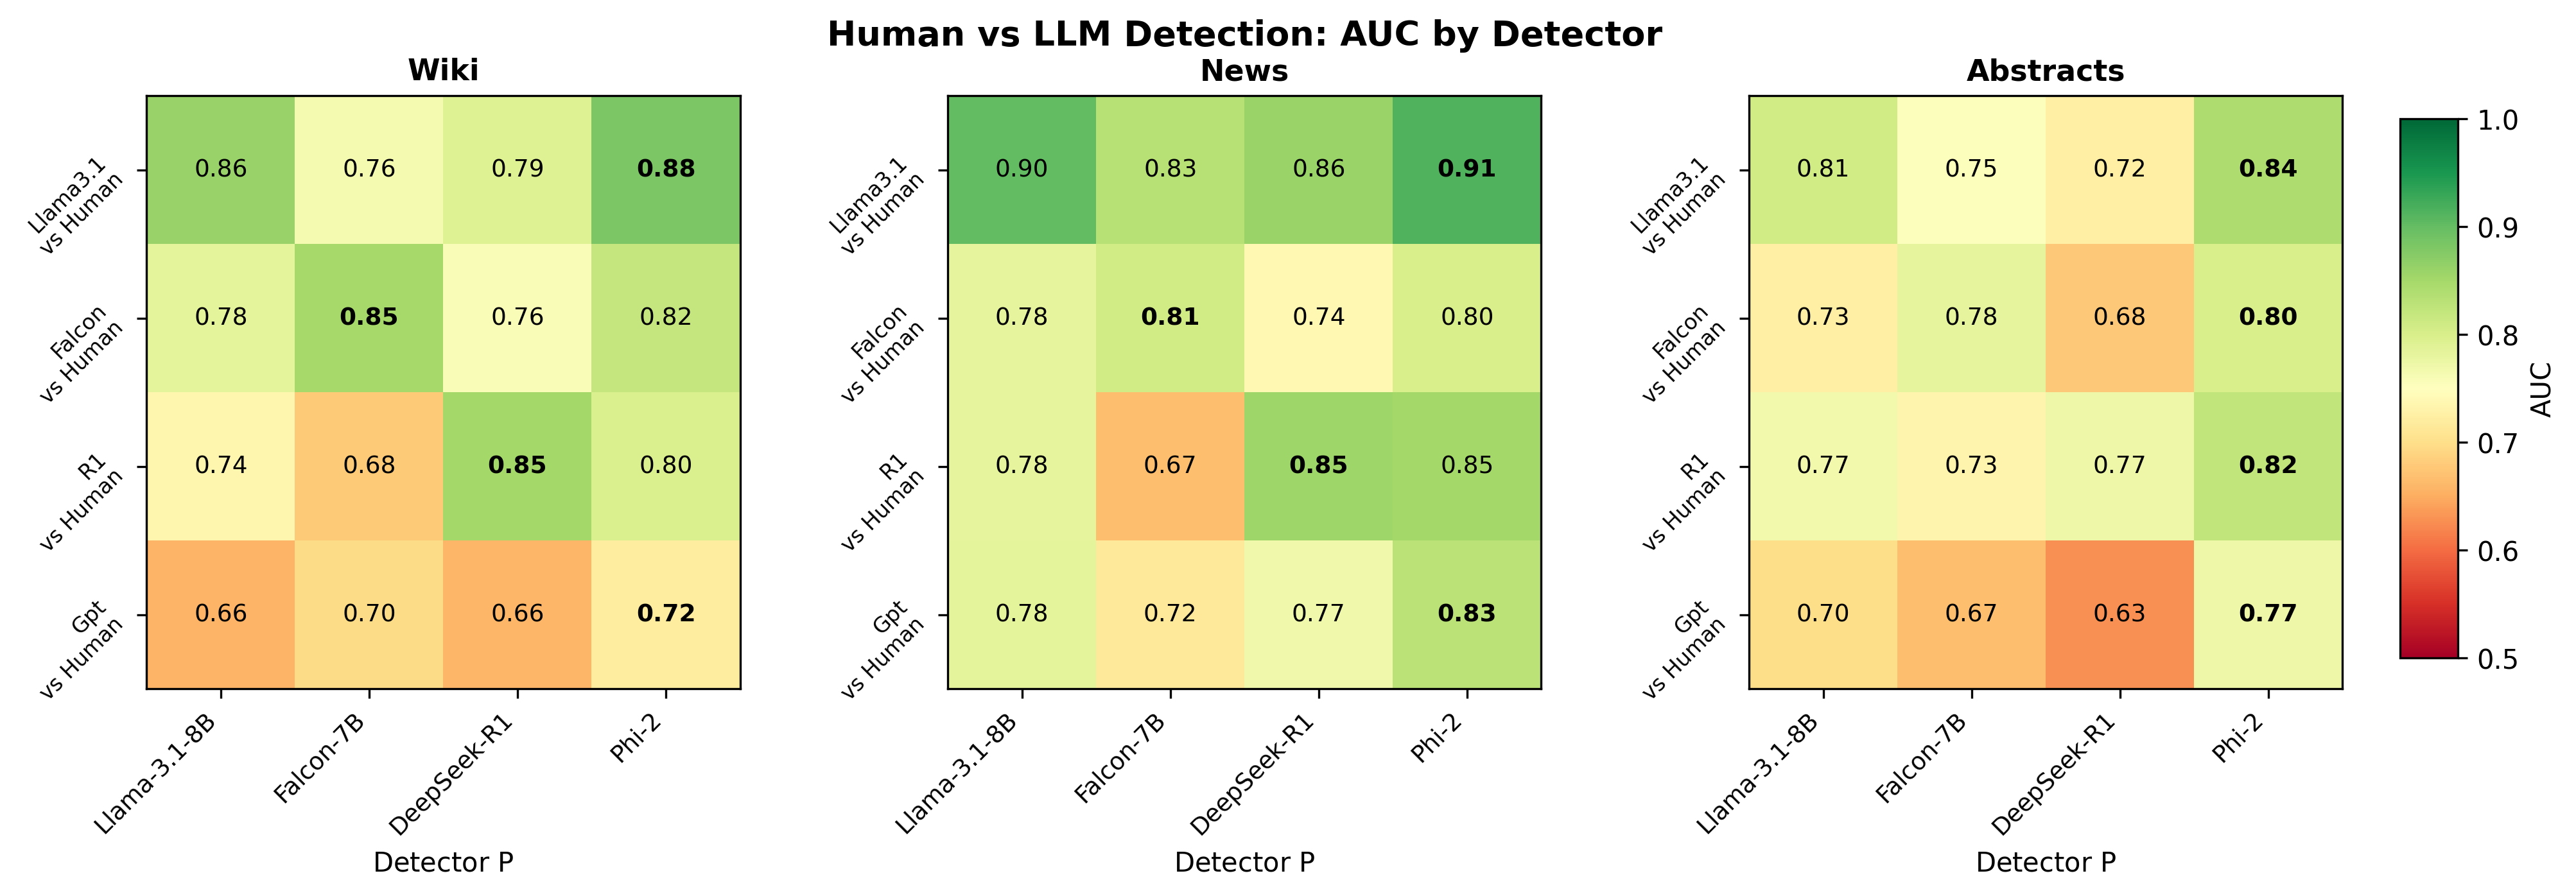
\includegraphics[width=0.96\linewidth, height=0.78\textheight, keepaspectratio]
    {figures/human_detection_heatmap.png}
\end{frame}

\end{document}
"
%   -> renders each slide with its speaker notes on the right (main_with_notes.pdf).
\providecommand{\WithNotes}{0}
\if\WithNotes1
  \usepackage{pgfpages}
  \setbeameroption{show notes on second screen=right}
\fi

% ---------- colours ----------
\definecolor{RUBlue}{RGB}{0, 74, 124}
\definecolor{RUAccent}{RGB}{0, 128, 180}
\definecolor{RUSoft}{RGB}{232, 241, 247}
\definecolor{RUInk}{RGB}{42, 53, 63}
\definecolor{LightGray}{RGB}{245, 245, 245}

\setbeamercolor{frametitle}{bg=RUBlue}
\setbeamercolor{progress bar}{fg=RUAccent}
\setbeamercolor{title separator}{fg=RUAccent}
\setbeamercolor{alerted text}{fg=RUAccent}
\setbeamercolor{normal text}{fg=RUInk}

% ---------- packages ----------
\usepackage{microtype}
\usepackage{amsmath, amssymb, mathtools}
\usepackage{graphicx}
\usepackage{booktabs}
\usepackage{tikz}
\usepackage{appendixnumberbeamer}
\usepackage[most]{tcolorbox}
\usetikzlibrary{arrows.meta, positioning, decorations.pathreplacing, calc, shapes.geometric}

% ---------- hyperref (configure existing beamer-loaded hyperref) ----------
\hypersetup{
  colorlinks=true,
  linkcolor=RUAccent,
  urlcolor=RUAccent,
  citecolor=RUAccent,
  pdftitle={Optimal Log-Likelihood Tests for Distinguishing Generative Models under Relative Entropy Constraints},
  pdfauthor={Adam Vinestock and Alon Kipnis},
}

% ---------- unified callout box ----------
\newtcolorbox{callout}[1][]{
  enhanced,
  colback=RUSoft,
  colframe=RUSoft,
  borderline west={2.4pt}{0pt}{RUAccent},
  boxrule=0pt,
  arc=2pt, outer arc=2pt,
  left=12pt, right=10pt, top=5pt, bottom=5pt,
  before skip=4pt, after skip=4pt,
  fontupper=\centering,
  width=\linewidth,
  #1
}

% ---------- thesis line ----------
\newcommand{\thesisline}[1]{%
  \begin{center}\large\color{RUAccent}#1\end{center}%
}

% ---------- macros ----------
\newcommand{\KL}[2]{D\!\left(#1 \,\middle\|\, #2\right)}
\newcommand{\Dkl}[2]{D(#1 \| #2)}
\newcommand{\Dchi}[2]{D_{\chi^2}(#1 \| #2)}
\newcommand{\bigDelta}{\Delta}
\newcommand{\cP}{\mathcal{P}}
\newcommand{\cG}{\mathcal{G}}
\newcommand{\cX}{\mathcal{X}}
\DeclareMathOperator*{\argmax}{arg\,max}
\DeclareMathOperator*{\argmin}{arg\,min}

% ---------- slide footer logos ----------
% Toggle: set to 0 (or comment out the \ifnum block below) to disable instantly.
\providecommand{\ShowSlideLogos}{1}
\newcommand{\SlideLogoHeight}{0.058\textheight}
\newcommand{\SlideLogoSepX}{1.4em}
\newcommand{\SlideLogoFootSep}{1.1ex}
\newcommand{\SlideLogoReichman}{figures/presentation/footer_reichman_logo.png}
\newcommand{\SlideLogoISIT}{figures/presentation/footer_isit_logo.png}
\ifnum\ShowSlideLogos=1
\setbeamertemplate{footline}{%
  \begin{beamercolorbox}[%
      wd=\paperwidth,%
      sep=\SlideLogoFootSep,%
      leftskip=\SlideLogoSepX,%
      rightskip=\SlideLogoSepX,%
    ]{footline}%
    \begin{minipage}[b]{0.28\paperwidth}%
      \raggedright
      \includegraphics[height=\SlideLogoHeight, keepaspectratio]{\SlideLogoReichman}%
    \end{minipage}%
    \hfill
    \begin{minipage}[b]{0.28\paperwidth}%
      \centering
      \usebeamerfont{page number in head/foot}%
      \usebeamertemplate*{frame numbering}%
    \end{minipage}%
    \hfill
    \begin{minipage}[b]{0.28\paperwidth}%
      \raggedleft
      \includegraphics[height=\SlideLogoHeight, keepaspectratio]{\SlideLogoISIT}%
    \end{minipage}%
  \end{beamercolorbox}%
}
% Logos only (no page number) for plain title/landing-style frames.
\newcommand{\SlideLogosOnly}{%
  \begin{tikzpicture}[remember picture, overlay]
    \node[anchor=south west, inner sep=0,
          xshift=\SlideLogoSepX, yshift=\SlideLogoFootSep]
      at (current page.south west) {%
        \includegraphics[height=\SlideLogoHeight, keepaspectratio]%
          {\SlideLogoReichman}%
    };
    \node[anchor=south east, inner sep=0,
          xshift=-\SlideLogoSepX, yshift=\SlideLogoFootSep]
      at (current page.south east) {%
        \includegraphics[height=\SlideLogoHeight, keepaspectratio]%
          {\SlideLogoISIT}%
    };
  \end{tikzpicture}%
}
\else
\newcommand{\SlideLogosOnly}{}
\fi

% ---------- metadata ----------
\title{Optimal Log-Likelihood Tests for Distinguishing\\
       Generative Models under Relative Entropy Constraints}
\subtitle{How to choose the detector model when the true source is out of reach}
\author{Adam Vinestock \and Alon Kipnis}
\institute{Reichman University, Herzliya, Israel}
\date{ISIT 2026}

% =================================================================
\begin{document}

% ------------------------------------------------------------------
% Frame 1 -- Title / promise
% ------------------------------------------------------------------
\begin{frame}[plain]
  \titlepage
  \SlideLogosOnly
\end{frame}

% ------------------------------------------------------------------
% Frame 2 -- Motivation: oracle unavailable, so a log-loss detector appears
% ------------------------------------------------------------------
\section{Motivation}
\begin{frame}{Testing When Model Likelihoods Are Inaccessible}
  \begin{columns}[c,onlytextwidth]
    \begin{column}{0.62\textwidth}
      \small
      \begin{itemize}
        \setlength\itemsep{0.5em}
        \item Was text \(X\) generated by \(G_0\), or by \(G_1\)?
        \item \textbf{Oracle test:} threshold the likelihood ratio
              \(\log \tfrac{G_1(x)}{G_0(x)}\).
        \item \textbf{Problem:} we can often \emph{sample}, not evaluate
              likelihoods (closed source, compute heavy, inaccessible).
        \item \textbf{Practical test:}
              evaluate logarithmic loss
              \(L(X;P)=\log \tfrac{1}{P(X)}\)
              under a third detector model \(P\)
              {\small(aka perplexity test).}
      \end{itemize}
    \end{column}
    \begin{column}{0.34\textwidth}
      \centering
      \hspace{0.45cm}%
      \begin{tikzpicture}[
          box/.style={
            rounded corners=2pt,
            draw=RUBlue,
            very thick,
            align=center,
            minimum width=3.4cm,
            minimum height=0.82cm,
            fill=RUSoft
          },
          arrow/.style={-{Latex[length=2.2mm]}, very thick, RUAccent}
        ]
        \node[box] (oracle) {oracle LR\\[-1pt]\(\log(G_1/G_0)\)};
        \node[box, below=0.55cm of oracle] (closed) {likelihoods\\unavailable};
        \node[box, below=0.55cm of closed] (detector) {evaluate\\\(L(X;P)\)};
        \draw[arrow] (oracle) -- (closed);
        \draw[arrow] (closed) -- (detector);
      \end{tikzpicture}
    \end{column}
  \end{columns}

  \vfill
  \vspace{0.25em}
  \begin{callout}
    \textbf{Goal: which detector \(P\) maximizes detection power?}\\[-1pt]
    {\small selected by an optimality criterion, not learned inside the test}
  \end{callout}
\end{frame}

% ------------------------------------------------------------------
% Frame 3 (merged) -- Example: empirical log-loss histograms + cites + thesis line.
% The former standalone formula frame is merged here; L(X;P) is now defined on Frame 2.
% Callout dropped; "The goal is maximum separation." kept.
% ------------------------------------------------------------------
\section{Detector}
\begin{frame}{Example: Log-Loss from Two Sources}
  \centering
  {\small Wikipedia sentences from two authors:
  \textbf{Falcon-7B} vs \textbf{Human}, under a third model \(P=\) \textbf{Phi-2}.}

  \vspace{0.1em}
  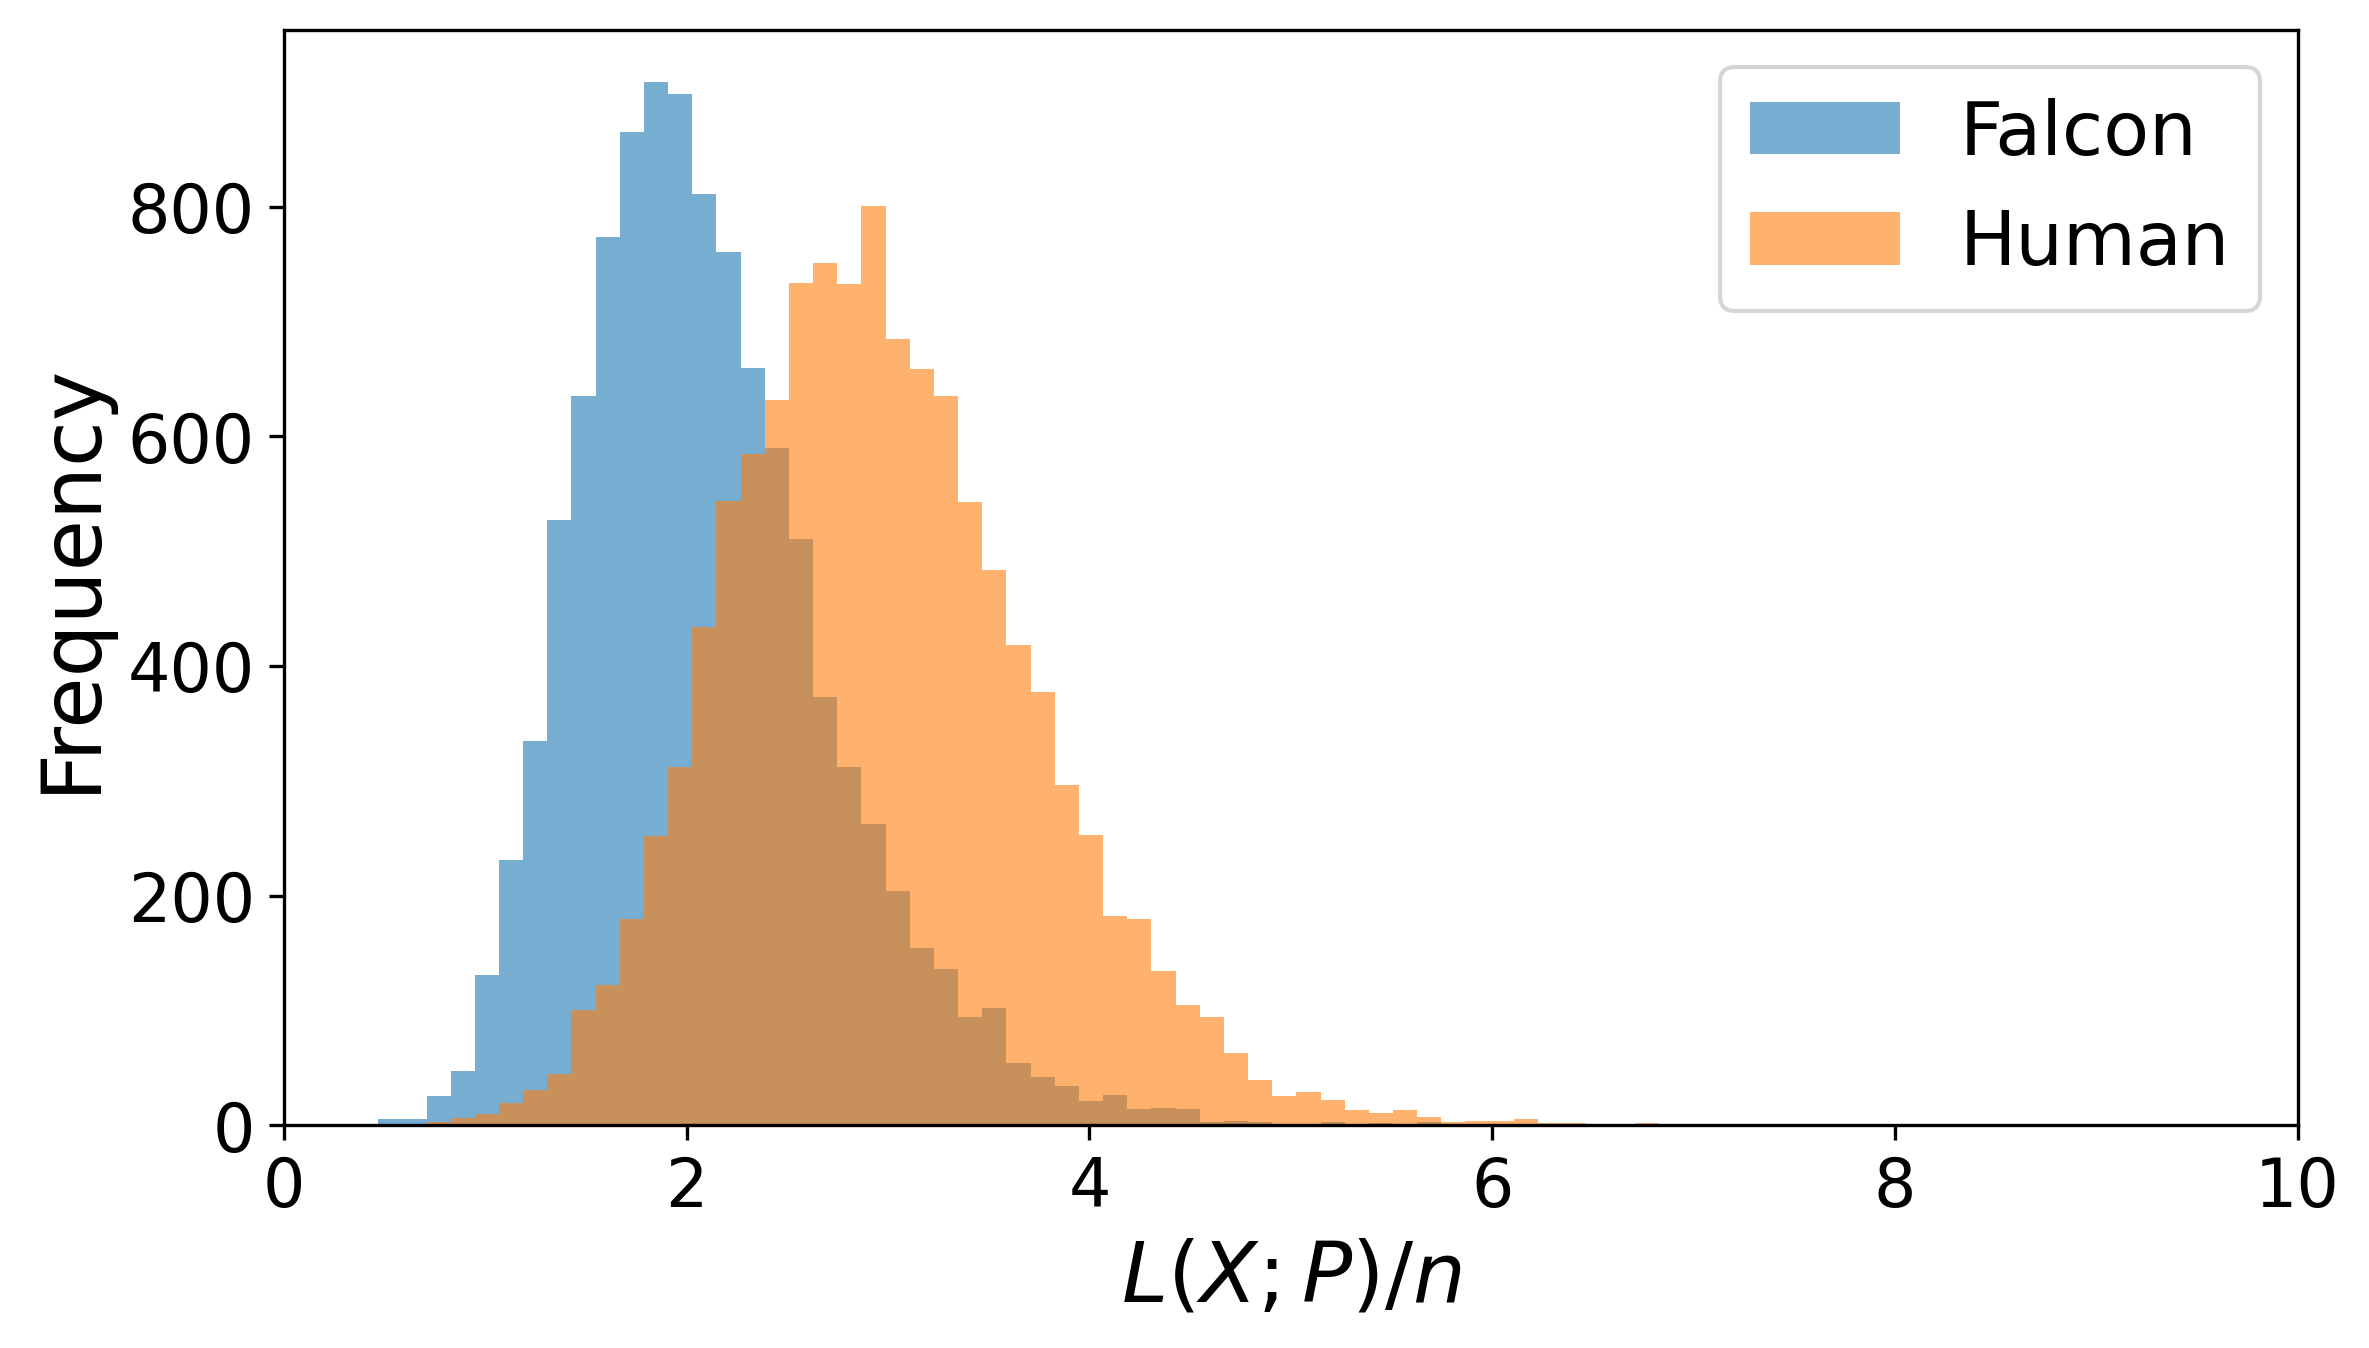
\includegraphics[width=\linewidth, height=0.57\textheight, keepaspectratio]
    {figures/presentation/response_hist_example_v2.png}

  \vspace{0.05em}
  {\scriptsize Related detectors: GLTR (Gehrmann et al., 2019),
   HowKGPT (Vasilatos et al., 2023), Binoculars (Hans et al., 2024).}

  \thesisline{The goal is maximum separation}
\end{frame}

% ------------------------------------------------------------------
% Frame 5 -- Related work
% ------------------------------------------------------------------
\begin{frame}{Related Work}
  \small
  \vfill
  Prior work addresses \textbf{adjacent problems} but not this
  \textbf{detector selection optimality question}:
  \vfill

  \begin{itemize}
    \setlength\itemsep{1.4em}

    \item \textbf{Unconstrained optimal detection} -
    Neyman-Pearson; Lehmann-Romano (2006)\\[-1pt]
    {\footnotesize When both models are known, thresholding the likelihood ratio
    \(\frac{G_1(X)}{G_0(X)}\) is optimal.}

    \item \textbf{Mismatched divergence} -
    Unnikrishnan, Huang, Meyn, Surana \& Veeravalli (2011)\\[-1pt]
    {\footnotesize Studies hypothesis testing when the ideal KL-based statistic
    is replaced by a mismatched one.}

    \item \textbf{M-projection / reverse I-projection} -
    Amari \& Nagaoka (2000)\\[-1pt]
    {\footnotesize Studies KL-based projection geometry over probability
    distributions; related to our objective, which is linear in
    \(\log p\).}

  \end{itemize}
  \vfill
\end{frame}

\note{
The oracle benchmark is Neyman-Pearson. Related work has studied
mismatched test statistics and KL projection geometry. Our work uses
this neighborhood of ideas, but applies it to choosing the detector model for
log-loss testing.
}

% ------------------------------------------------------------------
% Frame 6 -- Formal setup
% ------------------------------------------------------------------
\section{Setup}
\begin{frame}{Problem Setup}
  \begin{columns}[T,onlytextwidth]
    \begin{column}{0.60\textwidth}
      \textbf{Object:}\;
      \(X\) is the data sequence to attribute.

      \medskip
      \textbf{Hypothesis test:}
      \[
        H_0: X \sim G_0
        \qquad\text{vs.}\qquad
        H_1: X \sim G_1
      \]

      \textbf{Test statistic:}\;
      \(L(X;P) := \log \dfrac{1}{P(X)}\)

      \smallskip
      \textbf{Modeling assumption:}\; \(P\) lies near \(G_0\)
      {\small(shared tokenizer / architecture / training):}
      \[
        \boxed{P \in \cP_\epsilon(G_0)
               = \bigl\{P' : \Dkl{G_0}{P'} \leq \epsilon\bigr\}}
      \]

      {\small\textbf{Constrained optimality:}\; among detectors in this ball,
      we search for the one with maximum detection power.}
    \end{column}
    \hfill
    \begin{column}{0.36\textwidth}
      \centering
      \vspace{0.6em}
      \begin{tikzpicture}[scale=1.00]
        \shade[inner color=white, outer color=RUSoft]
              (0,0) circle (1.55cm);
        \draw[ultra thick, RUBlue] (0,0) circle (1.55cm);
        \node[RUBlue, font=\normalsize] at (0, 2.35)
             {\(\Dkl{G_0}{P}\!\leq\!\epsilon\)};
        \fill[RUBlue]   (0,0)      circle (2.5pt)
             node[below=5pt, font=\Large\bfseries]{\(G_0\)};
        \fill[orange!80!black] (2.55,1.3) circle (2.5pt)
             node[above right=-1pt, font=\large\bfseries]{\(G_1\)};
        \node[orange!80!black, font=\scriptsize, align=center] at (2.72,0.78)
             {alternative\\source};
        \fill[RUAccent] (0.65,0.82)  circle (2.5pt)
             node[right=3pt, font=\large\bfseries]{\(P\)};
        \fill[RUAccent] (-0.55,0.42) circle (2.5pt)
             node[left=3pt,  font=\large\bfseries]{\(P'\)};
        \fill[RUAccent] (0.35,-0.82) circle (2.5pt)
             node[right=3pt, font=\large\bfseries]{\(P''\)};
      \end{tikzpicture}
    \end{column}
  \end{columns}
\end{frame}

% ------------------------------------------------------------------
% Frame 7 -- Theorem 1: Delta controls power
% ------------------------------------------------------------------
\section{Main Result}
\begin{frame}{Result 1: Detector Power is Governed by \(\bigDelta\)}
  \small
  \textbf{Assumptions:} under \(G_0\) and \(G_1\), normalized log-loss is unimodal
  with variance stable across detectors.

  Power is monotone in the separation between the two log-loss distributions:
  \vspace{-0.25em}
  \[
    \mu_1(P)-\mu_0(P)
    =
    \underbrace{H(G_1)-H(G_0)}_{\text{fixed}}
    +
    \underbrace{\bigDelta(G_1,G_0;P)}_{\text{depends on }P}
  \]
  \vspace{-0.8em}
  {\Large
  \[
    \boxed{\bigDelta(G_1,G_0;P)
    :=\Dkl{G_1}{P}-\Dkl{G_0}{P}}
  \]
  }
  \vspace{-0.55em}

  \centering
  \begin{tikzpicture}[
      declare function={
        gauss(\x,\m,\s)=exp(-(\x-\m)^2/(2*\s^2))/(\s*sqrt(2*pi));
      }
    ]
    \begin{scope}[xscale=1.22, yscale=2.45]
      \draw[->, thick] (-3,0) -- (6.5,0)
           node[right, font=\footnotesize]{\(L(X;P)/n\)};
      \draw[RUBlue, very thick, domain=-3:3.8, samples=80]
           plot (\x, {gauss(\x,0,1)});
      \draw[red!70!black, very thick, domain=-0.8:6.5, samples=80]
           plot (\x, {gauss(\x,2.8,1)});
      \node[RUBlue, font=\small] at (0, 0.46)
           {\(\mu_0(P)\)};
      \node[red!70!black, font=\small] at (2.8, 0.46)
           {\(\mu_1(P)\)};
      \draw[<->, very thick, RUAccent]
           (0, -0.07) -- node[below, font=\small]
           {controlled by \(\bigDelta\)} (2.8, -0.07);
      \node[gray, font=\scriptsize, align=center] at (5.25, 0.32)
           {\(\sigma \approx\) stable\\[-1pt] across \(P\)};
    \end{scope}
  \end{tikzpicture}

  \vspace{-0.1em}
  \thesisline{Theorem~1: maximizing \(\bigDelta\) maximizes power at fixed Type-I level.}
\end{frame}

% ------------------------------------------------------------------
% Frame 8 -- Theorem 2: optimal detector for a simple alternative
% ------------------------------------------------------------------
\begin{frame}[t]{Result 2: Choosing the Optimal Detector \(P^*\)}
  \[
    \boxed{\vcenter{\hbox{$\displaystyle \max_{P \in \cP_\epsilon(G_0)}\;\bigDelta(G_1,G_0;P)$}}}
    \qquad\Longrightarrow\qquad
    \boxed{\vcenter{\hbox{$\displaystyle P^*(x)=G_0(x)-\gamma\bigl(G_1(x)-G_0(x)\bigr)$}}}
  \]
  \vspace{-0.3em}
  {\small\centering
  \textbf{Theorem 2:} \(P^*\) moves \alert{linearly away} from \(G_0\),
  opposite to \(G_1\), with \(D(G_0\|P^*)=\epsilon\).\par}

  \vspace{1.1em}
  \centering
  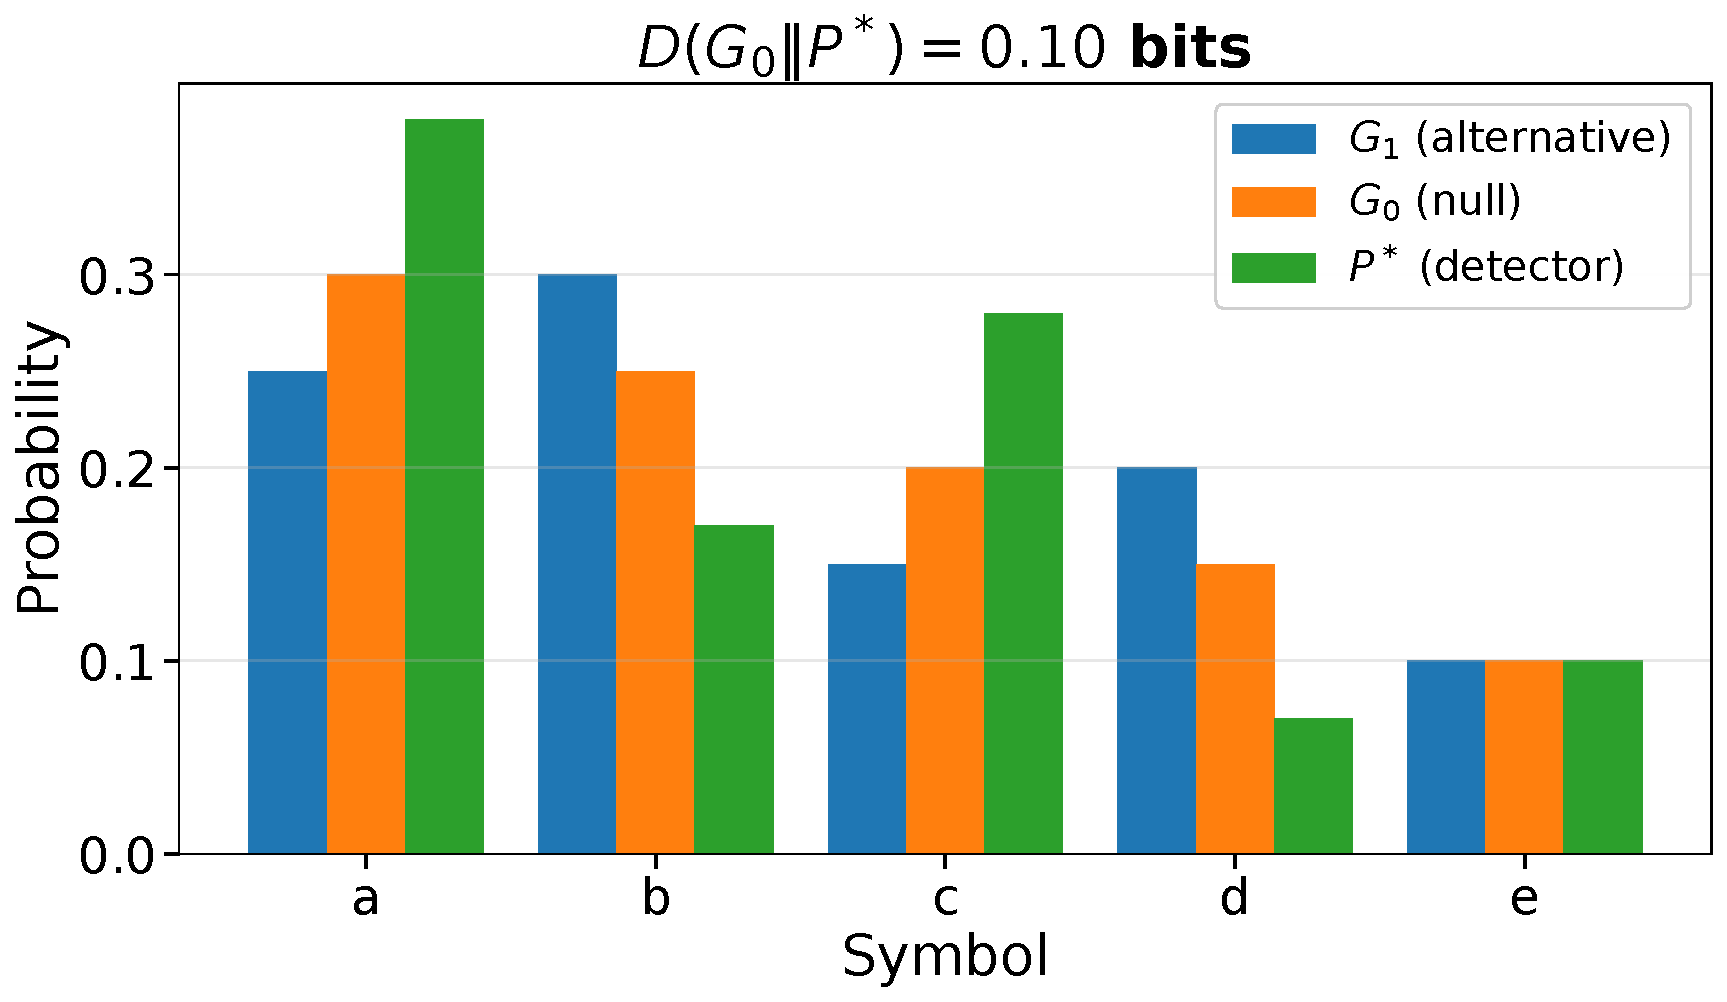
\includegraphics[width=0.80\linewidth, height=0.605\textheight, keepaspectratio]
    {figures/presentation/epsilon_ball_example.pdf}
\end{frame}

\note{
\textbf{Geometry of $P^*$ (Theorem 2).}
\begin{itemize}\small
  \item \textbf{The space is the probability simplex}: $G_0$, $G_1$, $P^*$ are
        each one point = a distribution over the alphabet. $G_1-G_0$ is the
        direction from $G_0$ toward $G_1$; $P^*$ steps the \emph{opposite} way
        (away from $G_1$) along a straight line.
  \item \textbf{Linear}, not geometric/exponential --- the small surprise of
        Thm~2. It subtracts mass from tokens where $G_1$ dominates, raising
        $-\log P$ there.
  \item $\epsilon$ = radius of the KL ball (the budget we choose); in the
        figure $\epsilon = 0.10$ bits --- that is exactly the
        ``$D(G_0\|P^*)=0.10$ bits'' label.
  \item $\gamma$ = step size in the formula; it is NOT free. Eq.~(10),
        $D(G_0\|P^*)=\epsilon$, pins $\gamma$ so $P^*$ lands exactly on the
        ball's boundary (constraint active, since $\Delta$ grows as we move
        away from $G_0$). So $\epsilon$ isn't written in eq.~(9): it enters
        through $\gamma$. Bigger $\epsilon\Rightarrow$ bigger
        $\gamma\Rightarrow P^*$ farther from $G_0$.
  \item \textbf{$\gamma\Leftrightarrow\epsilon$ relation:} no closed form in general
        (solve $\epsilon=-\sum_x G_0\log(1-\gamma\tfrac{G_1-G_0}{G_0})$,
        monotone in $\gamma$). Small-$\epsilon$:
        $\gamma\approx\sqrt{2\epsilon/\Dchi{G_1}{G_0}}$, i.e.
        $\gamma\propto\sqrt\epsilon$. This is the engine behind the
        Thm~3 gain $\sqrt{2\epsilon\,\Dchi{G_1}{G_0}}$.
        ($\epsilon$ in nats; $1/\ln2$ factor if in bits.)
\end{itemize}
}

% ------------------------------------------------------------------
% Frame 9 -- Composite alternatives and self-detection
% ------------------------------------------------------------------
\section{Composite Alternatives}
\begin{frame}[t]{Result 3: When Self-Detection is Locally Maximin-Optimal}
  \vspace{1.2em}
  \begin{columns}[c,onlytextwidth]
    \begin{column}{0.60\textwidth}
      {\small
      \textbf{Single \(G_1\):} move away from \(G_0\).\\[0.25em]
      \textbf{Family of alternatives \(\cG_1\):} optimize the worst case.}

      \[
        \bigDelta^*(\cG_1,G_0)=
        \sup_{P\in\cP_\epsilon(G_0)}\inf_{G\in\cG_1}\bigDelta(G,G_0;P)
      \]

      \vspace{0.5em}
      {\small \textbf{Modeling assumption:} LLM \(G_0\) can be viewed as a learned
      convex mixture of human-style sources:}

      \[
        G_0 \approx \sum_j \pi_j H_j
        \qquad \text{\footnotesize\(\pi_j\ge 0,\ \sum\nolimits_j \pi_j=1\)}
      \]
    \end{column}
    \hfill
    \begin{column}{0.39\textwidth}
      \centering
      \begin{tikzpicture}[scale=1.08]
        \fill[RUBlue] (0,0) circle (3pt)
             node[below=5pt, font=\normalsize]{$G_0$ {\footnotesize(LLM)}};
        \foreach \a in {0,20,...,340} {
          \pgfmathsetmacro{\r}{1.4+0.18*rand}
          \fill[red!50!black, opacity=0.55] (\a:\r) circle (1.8pt);
        }
        \draw[dashed, RUAccent, thick] (0,0) circle (1.6cm);
        \node[black, font=\small, align=center] at (0, -2.35)
             {alternative sources\\[-1pt] around \(G_0\)};
      \end{tikzpicture}
    \end{column}
  \end{columns}

  \vspace{0.15em}
  \begin{callout}[width=0.92\linewidth]
    {\small If alternatives \alert{isotropically surround} \(G_0\):}\\[2pt]
    {\Large \(\boldsymbol{P=G_0}\) is locally maximin optimal}
  \end{callout}
\end{frame}

% ------------------------------------------------------------------
% Frame 10 -- Empirical: normalized log-loss separation predicts AUC
% ------------------------------------------------------------------
\section{Evidence}
\begin{frame}[t]{Empirical Check: Normalized Separation Predicts AUC}
  \begin{columns}[c,onlytextwidth]
    \begin{column}{0.73\textwidth}
      \centering
      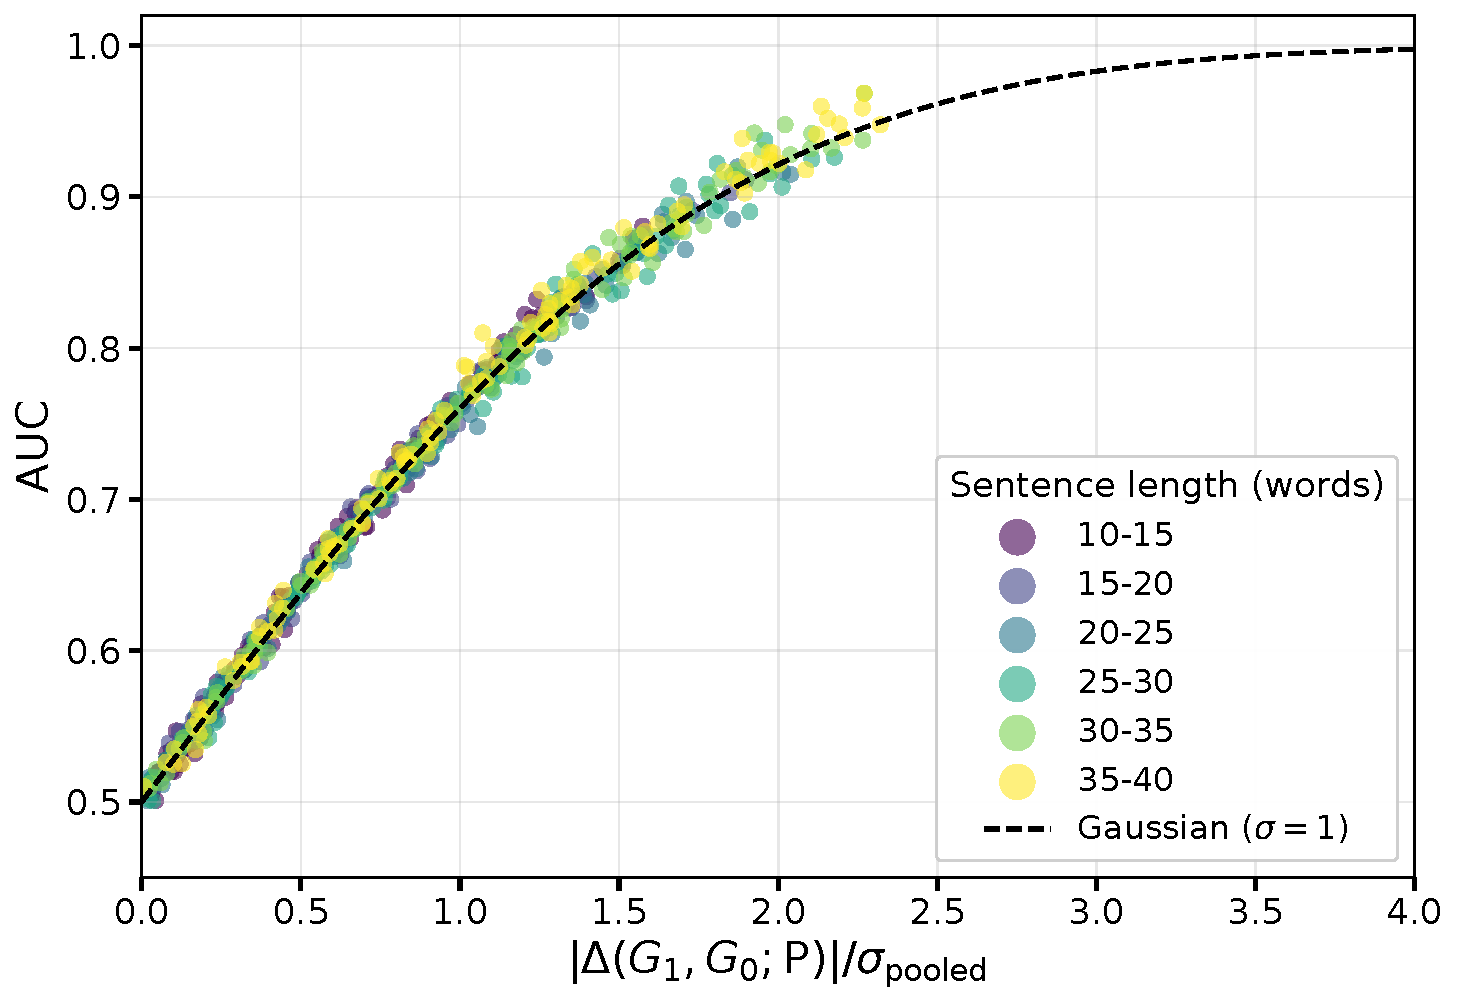
\includegraphics[width=\linewidth, height=0.625\textheight, keepaspectratio]
        {figures/presentation/auc_vs_delta_normalized_unified.pdf}
    \end{column}
    \hfill
    \begin{column}{0.25\textwidth}
      \small\textcolor{black!78}{%
      \(\displaystyle x:=\frac{|\hat\mu_1(P)-\hat\mu_0(P)|}{\hat\sigma_{\mathrm{pooled}}}\)\\[12pt]
      \(\mathrm{AUC}\approx\Phi(x/\sqrt{2})\)}
    \end{column}
  \end{columns}

  \vspace{0.3em}
  {\small \textbf{Experiment setup:} 275,000 sentences, 3 domains, 5 authors, 4 detector models}\\[2pt]
  {\small Empirical AUC follows the Gaussian curve:
  \alert{Pearson \(r=0.99\).}}\\[2pt]
  {\small\textcolor{RUBlue}{\textbf{Supports Result 1:}
  Gaussian-like log-loss behavior and stable variance.}}\\[2pt]
  {\footnotesize\textcolor{black!78}{Max/min standard-deviation ratio
  across detectors is \(1.2\)--\(1.5\times\).}}
\end{frame}

\note{
\textbf{VALIDATION, not a discovery.}
\begin{itemize}\small
  \item Don't pitch ``more separation $\to$ higher AUC'' as a finding ---
        obvious/monotone for any score.
  \item $\Phi(x/\sqrt2)$ = textbook binormal-AUC formula
        ($\mathrm{AUC}=\Pr(S_1>S_0)$ for two equal-variance Gaussians).
        We did NOT compute AUC with it: AUC is measured from the ROC
        (\texttt{roc\_auc\_score}); the curve is just overlaid. Parameter-free.
  \item Three claims tested: (1) $\Delta=D(G_1\|P)-D(G_0\|P)$ governs separation
        (Thm~1, not a priori obvious); (2) the unimodal, variance-stable
        Gaussian model (A1--A2) holds on real text; (3) the link is
        quantitative, not just directional.
  \item $r=0.99$ supports \textbf{A1--A2} (paper attributes Fig.~3 to A1--A2).
        \textbf{A3} ($\sigma$ independent of $P$) is checked \emph{separately}
        by the $1.2$--$1.5\times$ $\sigma$-ratio (Fig.~2). Single-$\sigma$ form
        assumes $\sigma_0\approx\sigma_1$; else
        $\Phi\!\big((\mu_1-\mu_0)/\sqrt{\sigma_0^2+\sigma_1^2}\big)$.
  \item Say: ``AUC measured from the ROC follows the parameter-free $\Phi(x/\sqrt2)$
        almost perfectly, so Thm~1's assumptions hold.'' Contribution = THEORY
        ($\Delta$ governs power; $P=G_0$ can be maximin); plot = credibility check.
\end{itemize}
}

% ------------------------------------------------------------------
% Frame 11 -- Human vs LLM evidence
% ------------------------------------------------------------------
\begin{frame}[t]{LLM vs.\ Human: Support for the Maximin Choice \(P=G_0\)}
  \centering
  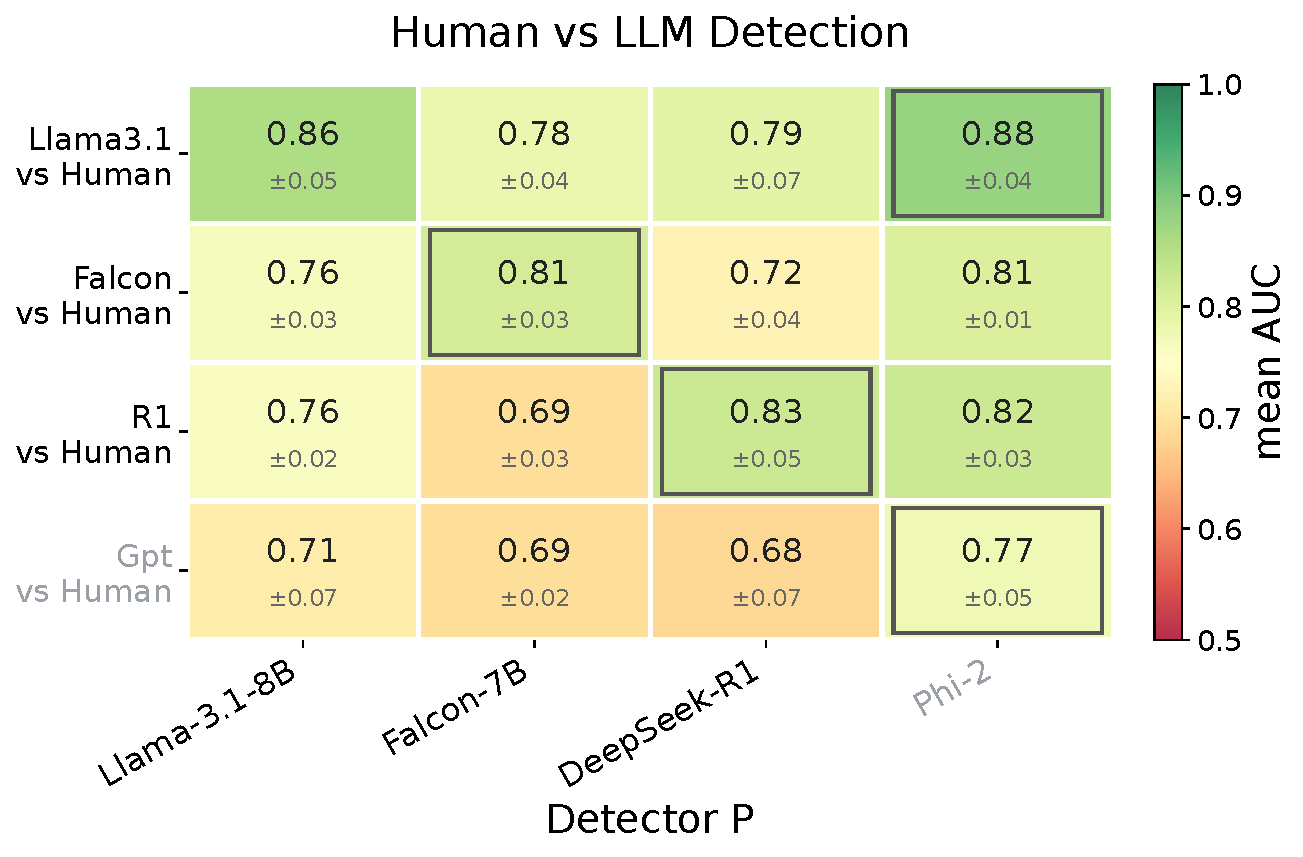
\includegraphics[width=0.98\linewidth, height=0.63\textheight, keepaspectratio]
    {figures/presentation/human_detection_heatmap_avg.pdf}

  \vfill
  \begin{columns}[c,onlytextwidth]
    \begin{column}{0.42\textwidth}
      \small\textbf{Matched detector \(P=G_0\):}
      \begin{itemize}
        \setlength\itemsep{0.1em}
        \item \alert{Best in 4/9} cases, second-best in 5/9
        \item Mean AUC \(\mathbf{0.831}\) vs.\ \(0.626\) for LLM-vs-LLM
      \end{itemize}
    \end{column}
    \hfill
    \begin{column}{0.55\textwidth}
      \begin{callout}[top=4pt,bottom=4pt,before skip=0pt,after skip=0pt,
          colframe=RUBlue!45, boxrule=0.5pt,
          borderline west={3pt}{0pt}{RUAccent}]
        \small Consistent with the maximin model if LLM \(G_0\) is surrounded
        by human sources.
      \end{callout}
    \end{column}
  \end{columns}
\end{frame}

% ------------------------------------------------------------------
% Frame 12 -- Contribution, not recap
% ------------------------------------------------------------------
\section{Takeaway}
\begin{frame}{Takeaway}
  \vfill
  \begin{enumerate}
    \setlength{\itemsep}{2.6em}
    \item When candidate-model likelihoods are unavailable,
          detect with a third model \(P\).

    \item The power-maximizing detector maximizes
          \(\bigDelta(G_1,G_0;P)=\Dkl{G_1}{P}-\Dkl{G_0}{P}\).

    \item For composite alternatives isotropically surrounding \(G_0\),
          self-detection is locally the maximin optimal choice.
  \end{enumerate}
  \vfill
\end{frame}

% ------------------------------------------------------------------
% Frame 13 -- Landing
% ------------------------------------------------------------------
{
\setbeamercolor{background canvas}{bg=RUBlue}
\setbeamercolor{normal text}{fg=white}
\usebeamercolor[fg]{normal text}
\hypersetup{urlcolor=white}
\begin{frame}[plain, c]
  \centering
  {\LARGE\textbf{Choose the detector. Maximize the gap.}}\\[1.8em]
  {\normalsize
    Adam Vinestock \quad\textbullet\quad
    \href{mailto:adam.vinestock@post.runi.ac.il}%
         {\texttt{adam.vinestock@post.runi.ac.il}}\\[3pt]
    Alon Kipnis \quad\textbullet\quad
    \href{mailto:alon.kipnis@runi.ac.il}%
         {\texttt{alon.kipnis@runi.ac.il}}
  }\\[1.4em]
  {\small Extended version \& proofs}\\[2pt]
  {\footnotesize\href{https://cs.idc.ac.il/~kipnis}%
                     {\texttt{cs.idc.ac.il/\~{}kipnis}}}
\end{frame}
}

% =================================================================
% BACKUP / APPENDIX
% =================================================================
\appendix
\metroset{numbering=none, progressbar=none}

% ------------------------------------------------------------------
% Backup B1 -- Theorem 3
% ------------------------------------------------------------------
\begin{frame}{How Sub-Optimal Is \(P=G_0\)?}
  Small-\(\epsilon\) expansion of the optimal gap:
  \[
    \bigDelta(G_1,G_0;P^*)
    =
    \Dkl{G_1}{G_0}
    +\sqrt{2\epsilon\,\Dchi{G_1}{G_0}}
    +O(\epsilon).
  \]

  \medskip
  \begin{callout}
    Deviating from \(G_0\) can raise the gap by
    \(\approx\sqrt{2\epsilon\,\Dchi{G_1}{G_0}}\),
    quantifying the sub-optimality of \(P=G_0\) against a
    \textbf{simple} alternative.
  \end{callout}

  \medskip
  \textbf{Where this comes from: the \(\gamma \Leftrightarrow \epsilon\) relation.}
  The constraint \(D(G_0\|P^*)=\epsilon\) fixes the step size \(\gamma\).
  It has no closed form in general, but for small \(\epsilon\)
  \[
    \epsilon \approx \tfrac{\gamma^2}{2}\,\Dchi{G_1}{G_0}
    \qquad\Longleftrightarrow\qquad
    \gamma \approx \sqrt{\tfrac{2\epsilon}{\Dchi{G_1}{G_0}}}
    \;\;(\gamma\propto\sqrt{\epsilon}),
  \]
  which substituted into the gap produces the
  \(\sqrt{2\epsilon\,\Dchi{G_1}{G_0}}\) term above.

  \medskip
  {\footnotesize Here
  \(\Dchi{G_1}{G_0}=\sum_x (G_1(x)-G_0(x))^2/G_0(x)\);
  \(\epsilon\) in nats (\(1/\ln2\) factor if measured in bits).}
\end{frame}

% ------------------------------------------------------------------
% Backup B2 -- Theorem 4
% ------------------------------------------------------------------
\begin{frame}{The Maximin Mechanism}
  For a composite family \(\cG_1\), the local maximin gap is set by
  a least-favorable prior \(\pi^*\):
  \[
    \bigDelta^*(\cG_1,G_0)
    =
    \mathbb{E}_{G\sim\pi^*}\!\left[\Dkl{G}{G_0}\right]
    +\sqrt{2\epsilon\,\Dchi{\bar G_{\pi^*}}{G_0}}
    +O(\epsilon),
  \]
  \[
    \bar G_{\pi^*}(x)=\mathbb{E}_{G\sim\pi^*}[G(x)].
  \]

  \begin{callout}
    If a non-convex alternative family isotropically surrounds \(G_0\),
    this mechanism yields Corollary 5.1: \(P=G_0\) is locally maximin.
  \end{callout}
\end{frame}

% ------------------------------------------------------------------
% Backup B2b -- Anisotropy index detail (definitions pushed off main slide 8)
% ------------------------------------------------------------------
\begin{frame}{Anisotropy Index and Isotropic Optimality}
  For a prior \(\pi^{\#}\) on \(\cG_1\) with \(G_0=\bar G_{\pi^{\#}}=\mathbb{E}_{G\sim\pi^{\#}}[G]\):
  \[
    \bar D_{\pi^{\#}}=\mathbb{E}_{G\sim\pi^{\#}}\Dkl{G}{G_0},
    \qquad
    r_{\pi^{\#}}=\sup_{G\in\operatorname{supp}(\pi^{\#})}
      \bigl|\Dkl{G}{G_0}-\bar D_{\pi^{\#}}\bigr|.
  \]
  \(r_{\pi^{\#}}=0\) iff all sources are equidistant from \(G_0\) in relative
  entropy (the mixture is isotropic); it grows with the unevenness of those
  distances.

  \medskip
  For any alternative \(G\in\cG_1\), the self-detector \(P=G_0\) obeys
  \[
    \bigDelta(G,G_0;G_0)=\Dkl{G}{G_0}
    \;\ge\;\bigDelta^*(\cG_1,G_0)-r_{\pi^{\#}}+O(\epsilon),
  \]
  so its worst-case sub-optimality is at most \(r_{\pi^{\#}}\). When
  \(r_{\pi^{\#}}=0\),
  \[
    \inf_{G\in\cG_1}\Dkl{G}{G_0}=\bigDelta^*(\cG_1,G_0)+O(\epsilon),
  \]
  i.e.\ \(P=G_0\) is locally maximin optimal.
\end{frame}

% ------------------------------------------------------------------
% Backup B3 -- Experimental setup
% ------------------------------------------------------------------
\begin{frame}{Experimental Setup}
  \begin{columns}[T,onlytextwidth]
    \begin{column}{0.48\textwidth}
      \textbf{Datasets} {\small(3 domains, matched topics)}
      \begin{itemize}
        \setlength\itemsep{0.25em}
        \item Wikipedia, News, Scientific abstracts
        \item \(\sim\!4{,}500\) docs, \(\sim\!275{,}000\) sentences
        \item Sentence length: 10--40 words
        \item Scored without preceding context
      \end{itemize}
    \end{column}
    \hfill
    \begin{column}{0.48\textwidth}
      \textbf{Authors / Detectors}
      \begin{itemize}
        \setlength\itemsep{0.25em}
        \item Authors: Llama-3.1, Falcon, GPT-3.5, DeepSeek-R1, Human
        \item Detectors \(P\): Llama-3.1, Falcon, Phi-2, DeepSeek-R1
        \item Some coincide \(\Rightarrow\) self-detection (\(P=G_0\))
      \end{itemize}
    \end{column}
  \end{columns}

  \vfill
  \begin{callout}
    GPT-3.5 model inaccessible for evaluation, so self-detection
    isn't possible.
  \end{callout}
\end{frame}

% ------------------------------------------------------------------
% Backup B4 -- Length confounding
% ------------------------------------------------------------------
\begin{frame}{Why Normalize?}
  \centering
  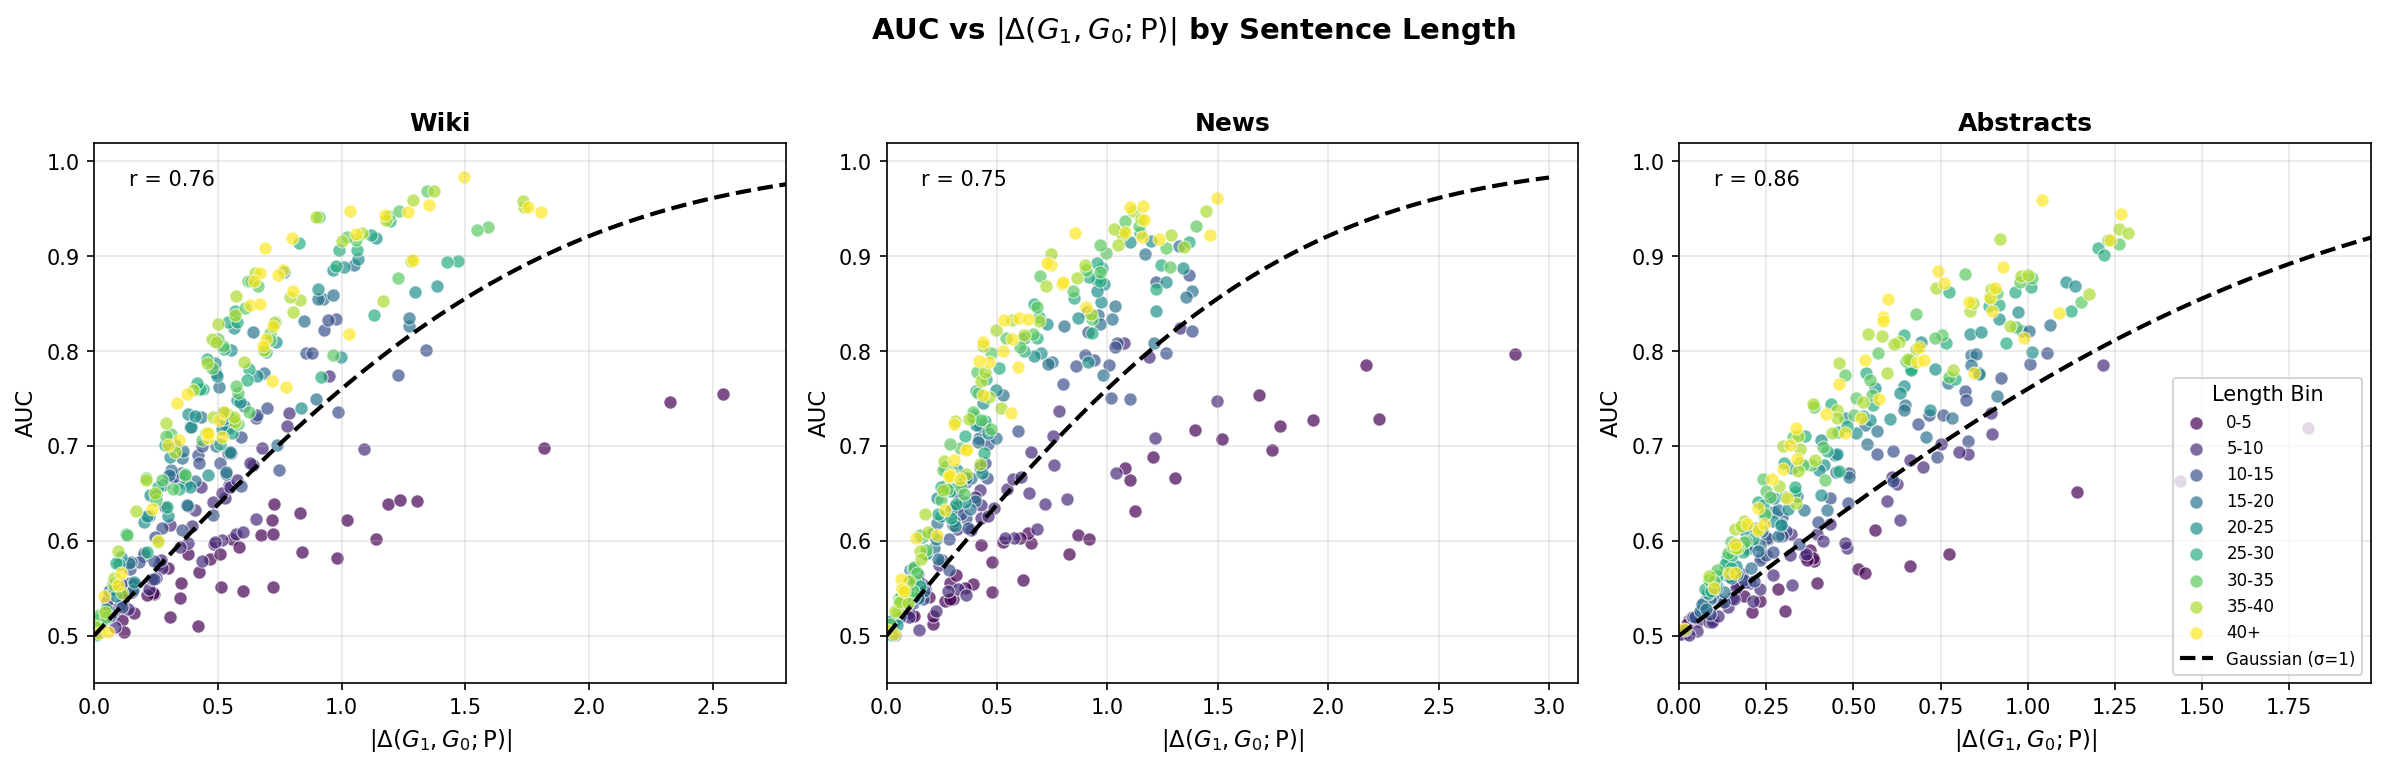
\includegraphics[width=0.95\linewidth, height=0.66\textheight, keepaspectratio]
    {figures/delta_auc_by_length.png}

  \vspace{0.3em}
  {\small Raw log-loss gaps are confounded by length. Dividing by
  \(\hat\sigma_{\mathrm{pooled}}\) collapses length bins onto the
  Gaussian AUC curve used in the main evidence slide.}
\end{frame}

% ------------------------------------------------------------------
% Backup B5 -- Variance stability
% ------------------------------------------------------------------
\begin{frame}{Variance Stability by Length}
  \centering
  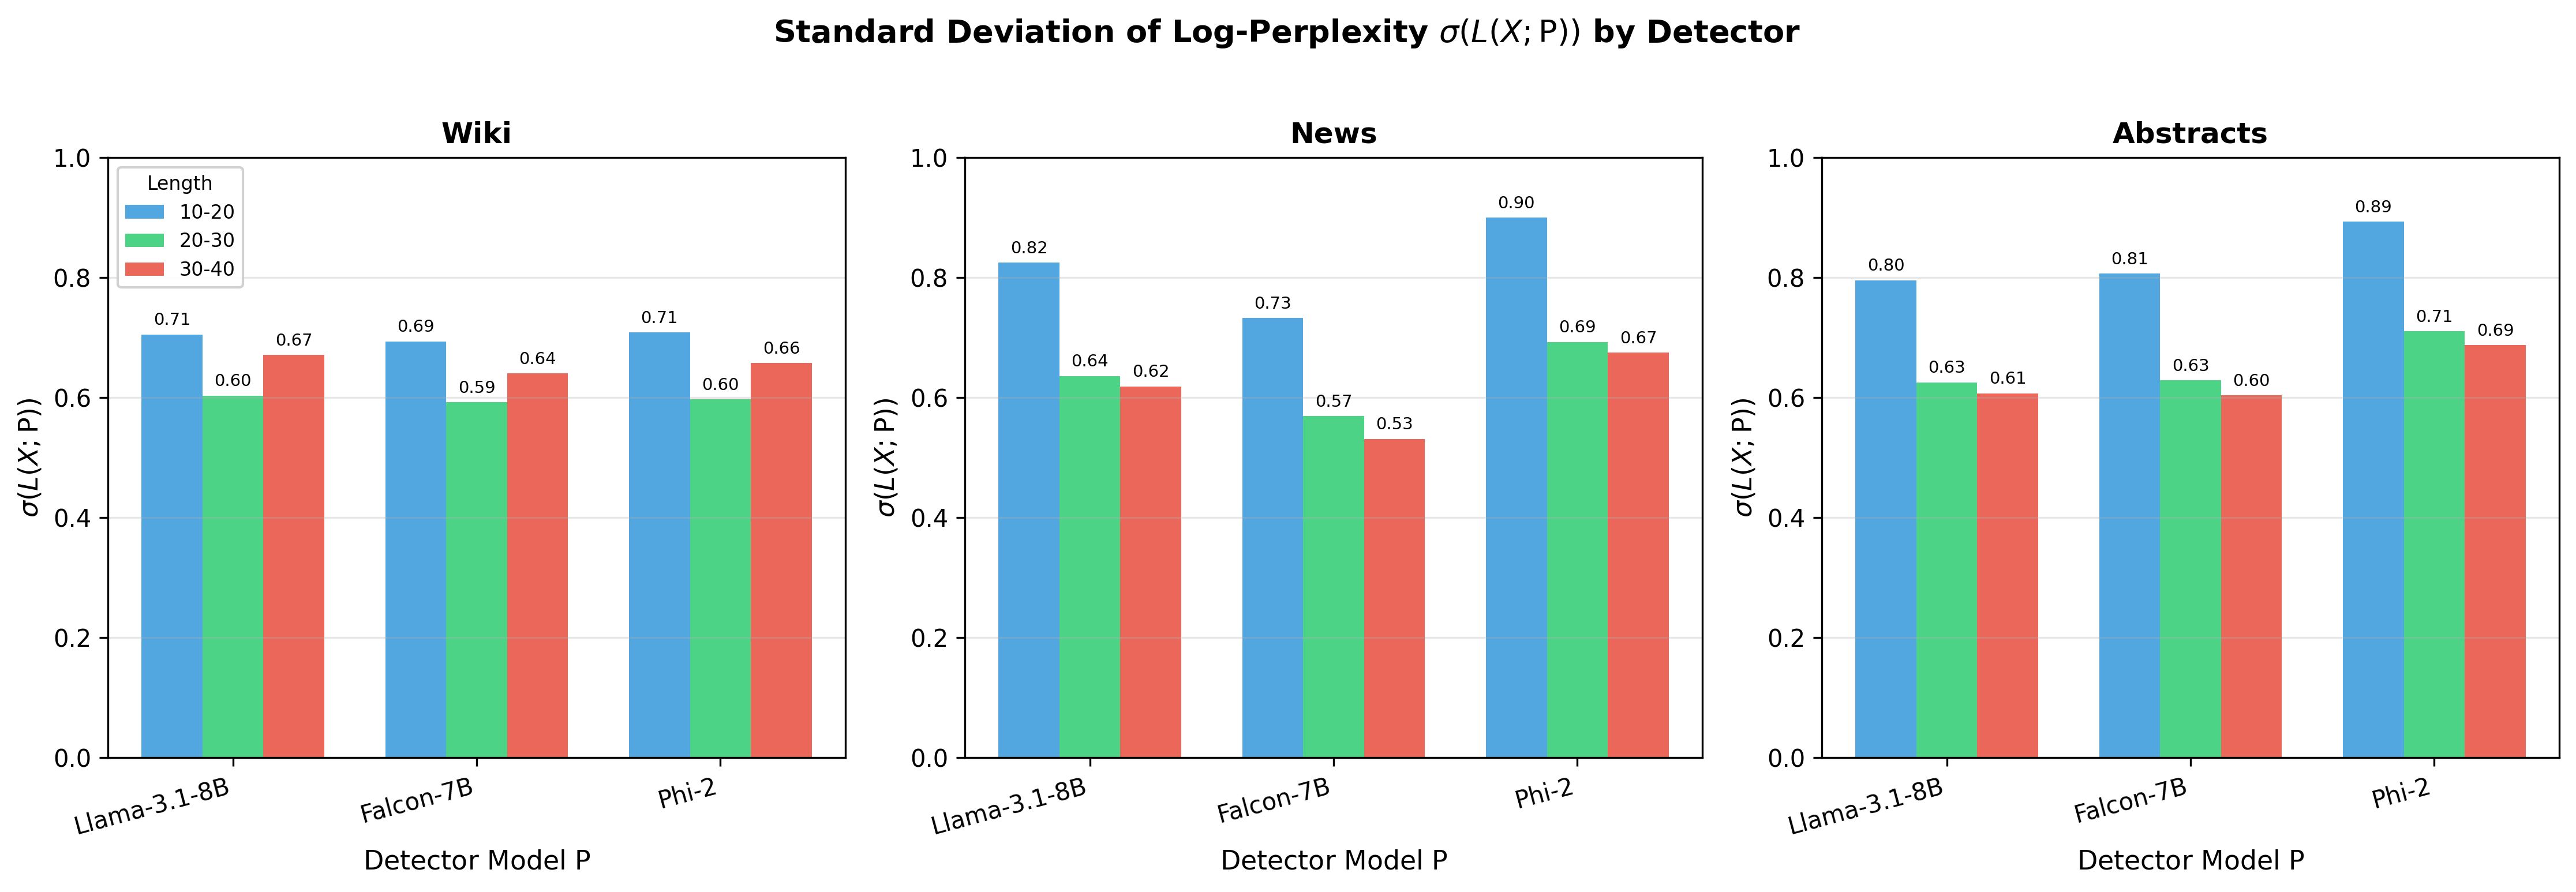
\includegraphics[width=\linewidth, height=0.62\textheight, keepaspectratio]
    {figures/sigma_vs_detector.png}

  \vspace{0.3em}
  {\small A3 view: standard deviation \(\sigma(L(X;P))\) by detector, split by
  sentence length. \emph{Within each length bin}, \(\sigma\) is nearly identical
  across Llama-3.1, Falcon, and Phi-2 (across-detector ratio \(\approx
  1.0\)--\(1.3\times\)), supporting A3; the larger spread within a dataset is
  driven by length, not by \(P\). DeepSeek-R1 is excluded as an outlier (its
  chat template inflates \(\sigma\)).}
\end{frame}

% ------------------------------------------------------------------
% Backup B6 -- Matched-detector counting
% ------------------------------------------------------------------
\begin{frame}{What ``Best in 4/9'' Means}
  \begin{itemize}
    \setlength\itemsep{0.55em}
    \item \textbf{The 9 cases:} 3 domains \(\times\) 3 matched LLM authors
          (Llama-3.1, Falcon, DeepSeek-R1).
    \item \textbf{GPT is excluded:} it has no corresponding open detector.
    \item \textbf{Phi-2 is detector-only:} it can win a heatmap cell, but
          is not part of the matched-detector count.
    \item \textbf{The claim:} among matched-detector cases,
          \(P=G_0\) is best in 4/9 and second-best in the remaining 5/9.
  \end{itemize}
\end{frame}

% ------------------------------------------------------------------
% Backup B7 -- AUC table
% ------------------------------------------------------------------
\begin{frame}{Matched-Detector AUC Numbers}
  \vfill
  \centering
  \textbf{AUC when detector matches source (\(P=G_0\))}

  \vspace{0.8em}
  \begin{tabular}{@{}lccc@{}}
    \toprule
    Dataset & Human vs.\ \(G_0\) & \(G_0\) vs.\ \(G_1\) & Gap \\
    \midrule
    Wiki      & \(0.853 \pm 0.006\) & \(0.659 \pm 0.065\) & \(+0.194\) \\
    News      & \(0.854 \pm 0.047\) & \(0.626 \pm 0.094\) & \(+0.229\) \\
    Abstracts & \(0.787 \pm 0.018\) & \(0.592 \pm 0.013\) & \(+0.195\) \\
    \midrule
    \textbf{Mean} & \(\mathbf{0.831}\) & \(\mathbf{0.626}\)
                  & \(\mathbf{+0.206}\) \\
    \bottomrule
  \end{tabular}

  \vspace{0.8em}
  {\small Human-vs-LLM self-detection is substantially easier than
  LLM-vs-LLM matched detection in this experiment.}
  \vfill
\end{frame}

% ------------------------------------------------------------------
% Backup B8--B10 -- Original (paper) versions of the updated plots
% ------------------------------------------------------------------
\begin{frame}{Backup: Original \(P^*\) Example (paper figure)}
  \centering
  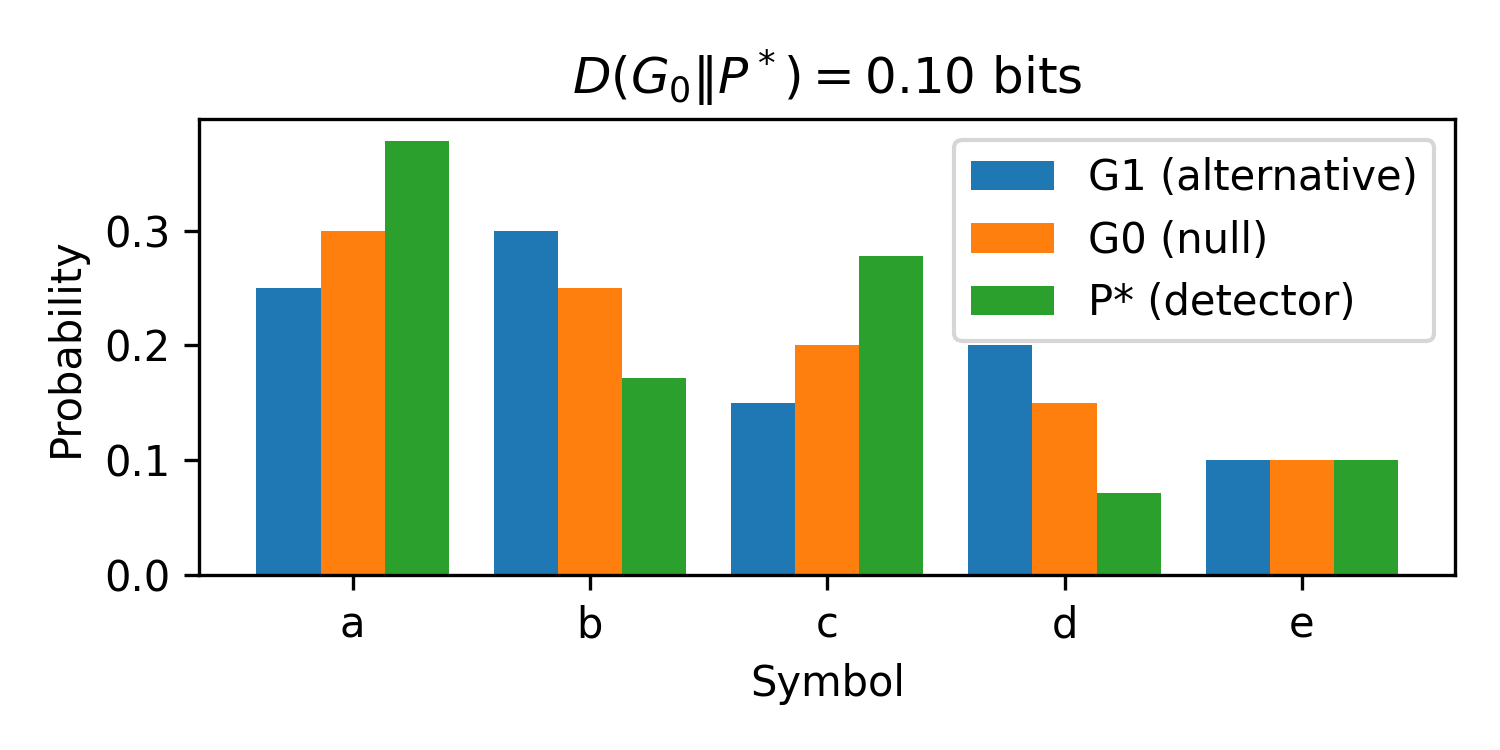
\includegraphics[width=0.92\linewidth, height=0.74\textheight, keepaspectratio]
    {figures/epsilon_ball_example.png}
\end{frame}

\begin{frame}{Backup: Original AUC vs Normalized Separation (paper figure)}
  \centering
  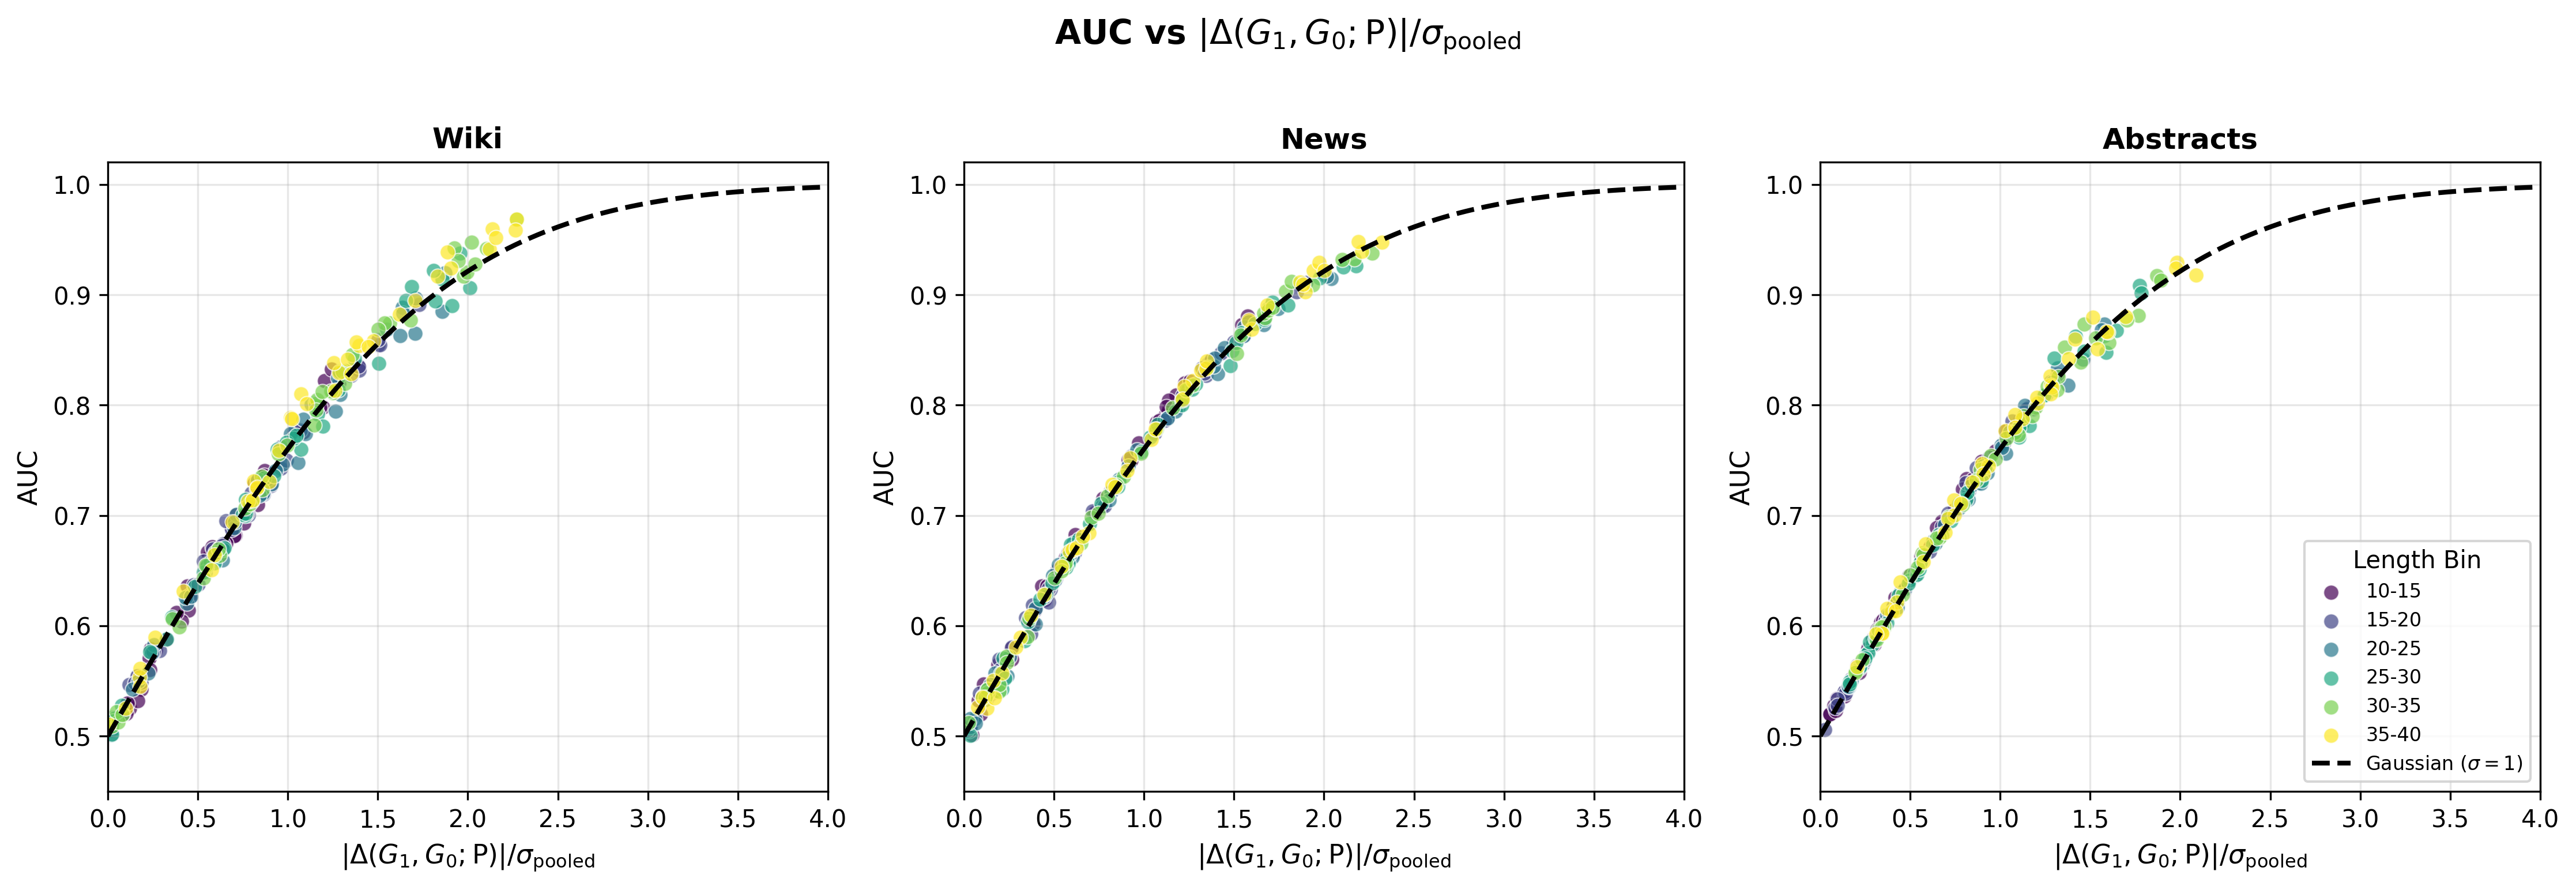
\includegraphics[width=0.96\linewidth, height=0.78\textheight, keepaspectratio]
    {figures/auc_vs_delta_normalized.png}
\end{frame}

\begin{frame}{Backup: Original Human-vs-LLM Heatmap (paper figure)}
  \centering
  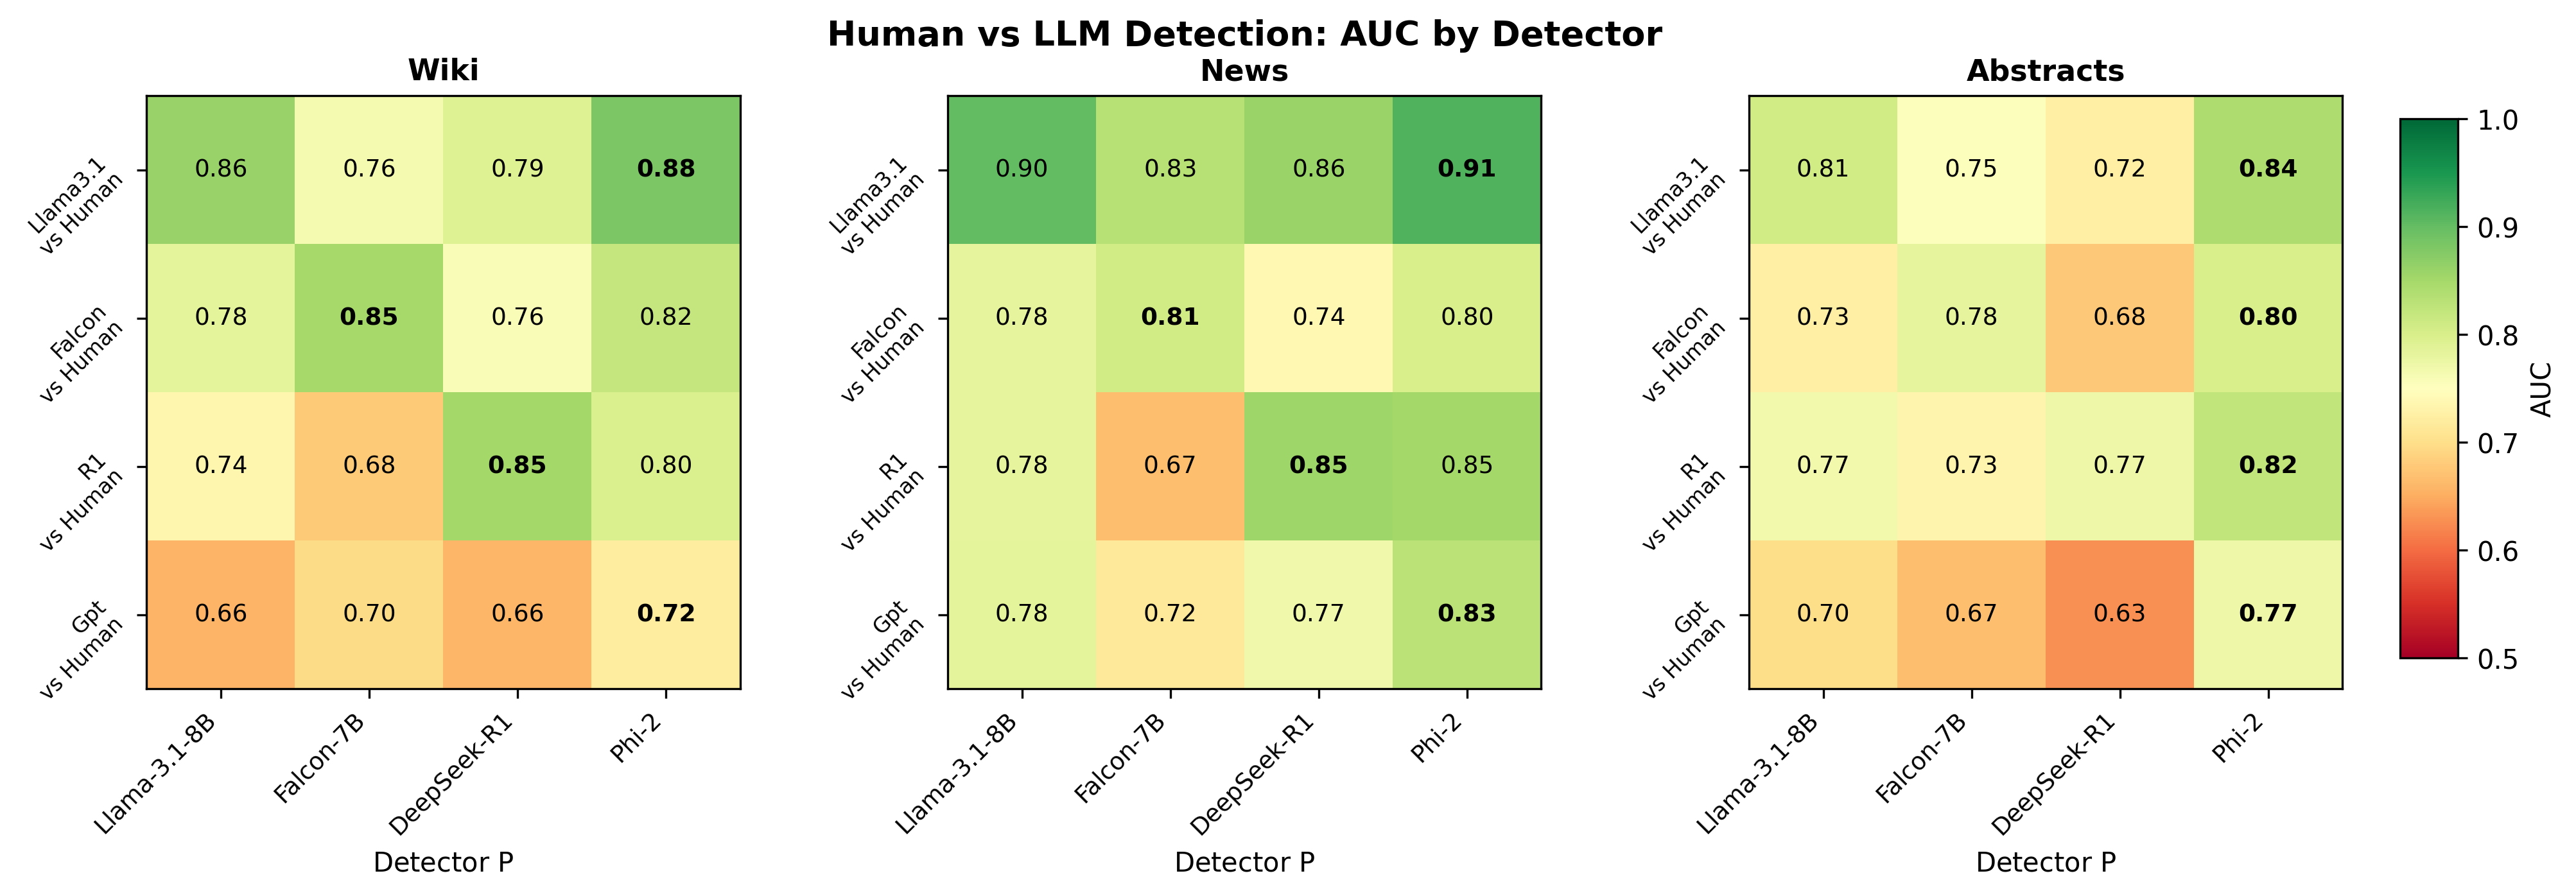
\includegraphics[width=0.96\linewidth, height=0.78\textheight, keepaspectratio]
    {figures/human_detection_heatmap.png}
\end{frame}

\end{document}
"
%   -> renders each slide with its speaker notes on the right (main_with_notes.pdf).
\providecommand{\WithNotes}{0}
\if\WithNotes1
  \usepackage{pgfpages}
  \setbeameroption{show notes on second screen=right}
\fi

% ---------- colours ----------
\definecolor{RUBlue}{RGB}{0, 74, 124}
\definecolor{RUAccent}{RGB}{0, 128, 180}
\definecolor{RUSoft}{RGB}{232, 241, 247}
\definecolor{RUInk}{RGB}{42, 53, 63}
\definecolor{LightGray}{RGB}{245, 245, 245}

\setbeamercolor{frametitle}{bg=RUBlue}
\setbeamercolor{progress bar}{fg=RUAccent}
\setbeamercolor{title separator}{fg=RUAccent}
\setbeamercolor{alerted text}{fg=RUAccent}
\setbeamercolor{normal text}{fg=RUInk}

% ---------- packages ----------
\usepackage{microtype}
\usepackage{amsmath, amssymb, mathtools}
\usepackage{graphicx}
\usepackage{booktabs}
\usepackage{tikz}
\usepackage{appendixnumberbeamer}
\usepackage[most]{tcolorbox}
\usetikzlibrary{arrows.meta, positioning, decorations.pathreplacing, calc, shapes.geometric}

% ---------- hyperref (configure existing beamer-loaded hyperref) ----------
\hypersetup{
  colorlinks=true,
  linkcolor=RUAccent,
  urlcolor=RUAccent,
  citecolor=RUAccent,
  pdftitle={Optimal Log-Likelihood Tests for Distinguishing Generative Models under Relative Entropy Constraints},
  pdfauthor={Adam Vinestock and Alon Kipnis},
}

% ---------- unified callout box ----------
\newtcolorbox{callout}[1][]{
  enhanced,
  colback=RUSoft,
  colframe=RUSoft,
  borderline west={2.4pt}{0pt}{RUAccent},
  boxrule=0pt,
  arc=2pt, outer arc=2pt,
  left=12pt, right=10pt, top=5pt, bottom=5pt,
  before skip=4pt, after skip=4pt,
  fontupper=\centering,
  width=\linewidth,
  #1
}

% ---------- thesis line ----------
\newcommand{\thesisline}[1]{%
  \begin{center}\large\color{RUAccent}#1\end{center}%
}

% ---------- macros ----------
\newcommand{\KL}[2]{D\!\left(#1 \,\middle\|\, #2\right)}
\newcommand{\Dkl}[2]{D(#1 \| #2)}
\newcommand{\Dchi}[2]{D_{\chi^2}(#1 \| #2)}
\newcommand{\bigDelta}{\Delta}
\newcommand{\cP}{\mathcal{P}}
\newcommand{\cG}{\mathcal{G}}
\newcommand{\cX}{\mathcal{X}}
\DeclareMathOperator*{\argmax}{arg\,max}
\DeclareMathOperator*{\argmin}{arg\,min}

% ---------- slide footer logos ----------
% Toggle: set to 0 (or comment out the \ifnum block below) to disable instantly.
\providecommand{\ShowSlideLogos}{1}
\newcommand{\SlideLogoHeight}{0.058\textheight}
\newcommand{\SlideLogoSepX}{1.4em}
\newcommand{\SlideLogoFootSep}{1.1ex}
\newcommand{\SlideLogoReichman}{figures/presentation/footer_reichman_logo.png}
\newcommand{\SlideLogoISIT}{figures/presentation/footer_isit_logo.png}
\ifnum\ShowSlideLogos=1
\setbeamertemplate{footline}{%
  \begin{beamercolorbox}[%
      wd=\paperwidth,%
      sep=\SlideLogoFootSep,%
      leftskip=\SlideLogoSepX,%
      rightskip=\SlideLogoSepX,%
    ]{footline}%
    \begin{minipage}[b]{0.28\paperwidth}%
      \raggedright
      \includegraphics[height=\SlideLogoHeight, keepaspectratio]{\SlideLogoReichman}%
    \end{minipage}%
    \hfill
    \begin{minipage}[b]{0.28\paperwidth}%
      \centering
      \usebeamerfont{page number in head/foot}%
      \usebeamertemplate*{frame numbering}%
    \end{minipage}%
    \hfill
    \begin{minipage}[b]{0.28\paperwidth}%
      \raggedleft
      \includegraphics[height=\SlideLogoHeight, keepaspectratio]{\SlideLogoISIT}%
    \end{minipage}%
  \end{beamercolorbox}%
}
% Logos only (no page number) for plain title/landing-style frames.
\newcommand{\SlideLogosOnly}{%
  \begin{tikzpicture}[remember picture, overlay]
    \node[anchor=south west, inner sep=0,
          xshift=\SlideLogoSepX, yshift=\SlideLogoFootSep]
      at (current page.south west) {%
        \includegraphics[height=\SlideLogoHeight, keepaspectratio]%
          {\SlideLogoReichman}%
    };
    \node[anchor=south east, inner sep=0,
          xshift=-\SlideLogoSepX, yshift=\SlideLogoFootSep]
      at (current page.south east) {%
        \includegraphics[height=\SlideLogoHeight, keepaspectratio]%
          {\SlideLogoISIT}%
    };
  \end{tikzpicture}%
}
\else
\newcommand{\SlideLogosOnly}{}
\fi

% ---------- metadata ----------
\title{Optimal Log-Likelihood Tests for Distinguishing\\
       Generative Models under Relative Entropy Constraints}
\subtitle{How to choose the detector model when the true source is out of reach}
\author{Adam Vinestock \and Alon Kipnis}
\institute{Reichman University, Herzliya, Israel}
\date{ISIT 2026}

% =================================================================
\begin{document}

% ------------------------------------------------------------------
% Frame 1 -- Title / promise
% ------------------------------------------------------------------
\begin{frame}[plain]
  \titlepage
  \SlideLogosOnly
\end{frame}

% ------------------------------------------------------------------
% Frame 2 -- Motivation: oracle unavailable, so a log-loss detector appears
% ------------------------------------------------------------------
\section{Motivation}
\begin{frame}{Testing When Model Likelihoods Are Inaccessible}
  \begin{columns}[c,onlytextwidth]
    \begin{column}{0.62\textwidth}
      \small
      \begin{itemize}
        \setlength\itemsep{0.5em}
        \item Was text \(X\) generated by \(G_0\), or by \(G_1\)?
        \item \textbf{Oracle test:} threshold the likelihood ratio
              \(\log \tfrac{G_1(x)}{G_0(x)}\).
        \item \textbf{Problem:} we can often \emph{sample}, not evaluate
              likelihoods (closed source, compute heavy, inaccessible).
        \item \textbf{Practical test:}
              evaluate logarithmic loss
              \(L(X;P)=\log \tfrac{1}{P(X)}\)
              under a third detector model \(P\)
              {\small(aka perplexity test).}
      \end{itemize}
    \end{column}
    \begin{column}{0.34\textwidth}
      \centering
      \hspace{0.45cm}%
      \begin{tikzpicture}[
          box/.style={
            rounded corners=2pt,
            draw=RUBlue,
            very thick,
            align=center,
            minimum width=3.4cm,
            minimum height=0.82cm,
            fill=RUSoft
          },
          arrow/.style={-{Latex[length=2.2mm]}, very thick, RUAccent}
        ]
        \node[box] (oracle) {oracle LR\\[-1pt]\(\log(G_1/G_0)\)};
        \node[box, below=0.55cm of oracle] (closed) {likelihoods\\unavailable};
        \node[box, below=0.55cm of closed] (detector) {evaluate\\\(L(X;P)\)};
        \draw[arrow] (oracle) -- (closed);
        \draw[arrow] (closed) -- (detector);
      \end{tikzpicture}
    \end{column}
  \end{columns}

  \vfill
  \vspace{0.25em}
  \begin{callout}
    \textbf{Goal: which detector \(P\) maximizes detection power?}\\[-1pt]
    {\small selected by an optimality criterion, not learned inside the test}
  \end{callout}
\end{frame}

% ------------------------------------------------------------------
% Frame 3 (merged) -- Example: empirical log-loss histograms + cites + thesis line.
% The former standalone formula frame is merged here; L(X;P) is now defined on Frame 2.
% Callout dropped; "The goal is maximum separation." kept.
% ------------------------------------------------------------------
\section{Detector}
\begin{frame}{Example: Log-Loss from Two Sources}
  \centering
  {\small Wikipedia sentences from two authors:
  \textbf{Falcon-7B} vs \textbf{Human}, under a third model \(P=\) \textbf{Phi-2}.}

  \vspace{0.1em}
  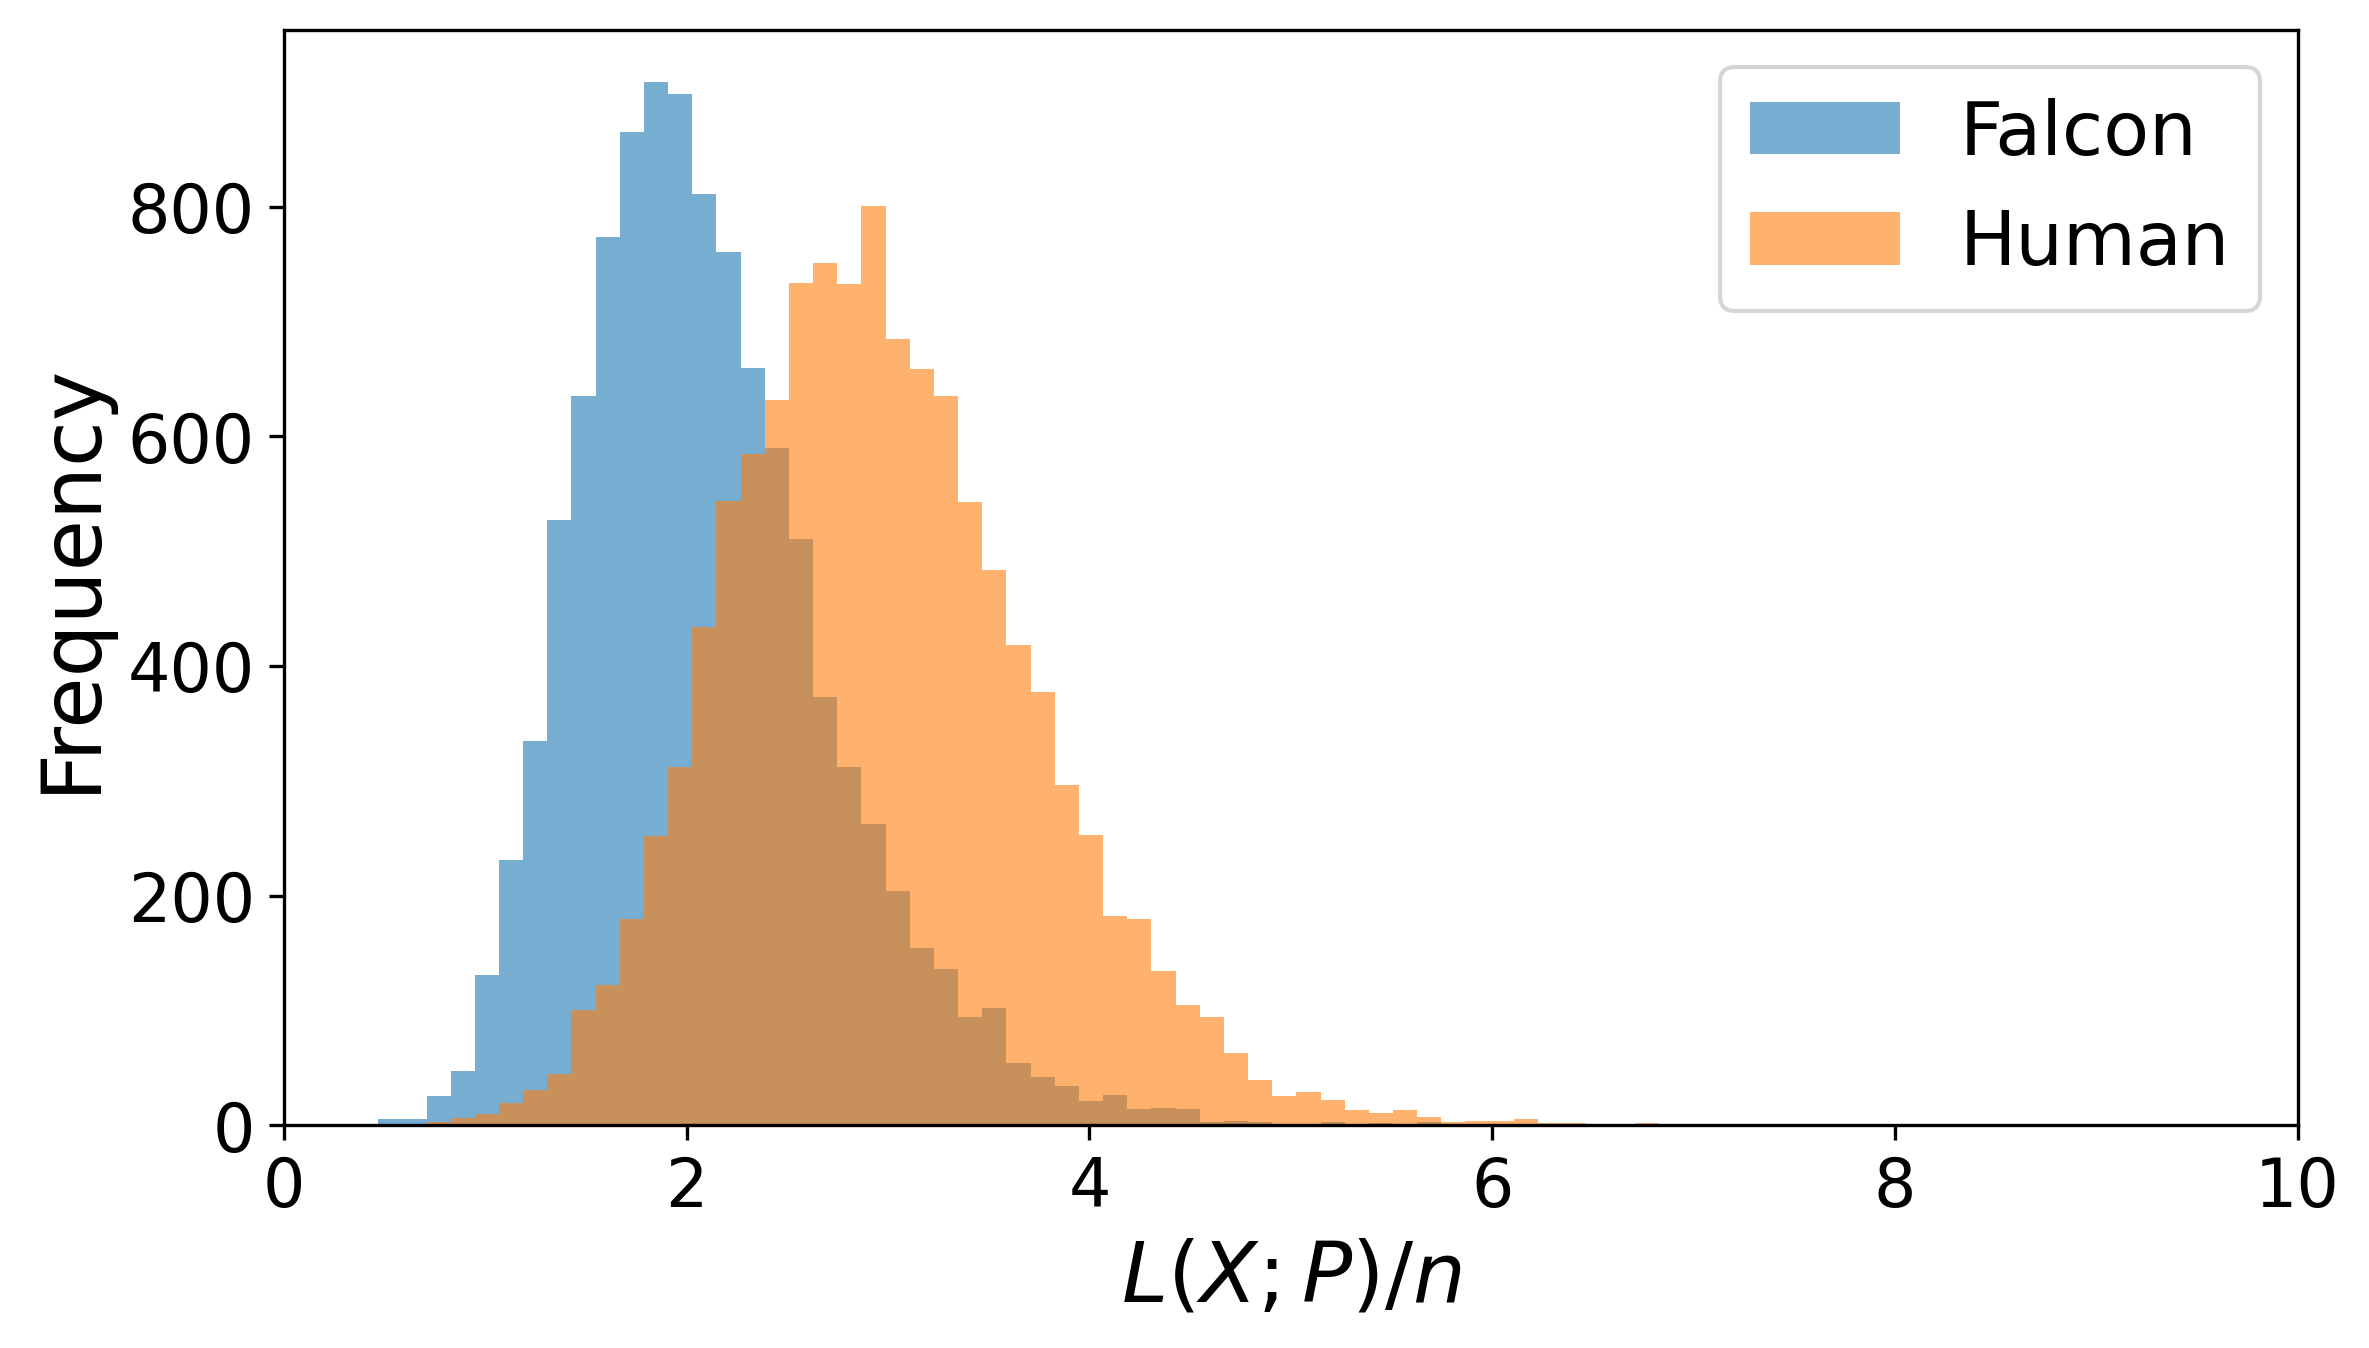
\includegraphics[width=\linewidth, height=0.57\textheight, keepaspectratio]
    {figures/presentation/response_hist_example_v2.png}

  \vspace{0.05em}
  {\scriptsize Related detectors: GLTR (Gehrmann et al., 2019),
   HowKGPT (Vasilatos et al., 2023), Binoculars (Hans et al., 2024).}

  \thesisline{The goal is maximum separation}
\end{frame}

% ------------------------------------------------------------------
% Frame 5 -- Related work
% ------------------------------------------------------------------
\begin{frame}{Related Work}
  \small
  \vfill
  Prior work addresses \textbf{adjacent problems} but not this
  \textbf{detector selection optimality question}:
  \vfill

  \begin{itemize}
    \setlength\itemsep{1.4em}

    \item \textbf{Unconstrained optimal detection} -
    Neyman-Pearson; Lehmann-Romano (2006)\\[-1pt]
    {\footnotesize When both models are known, thresholding the likelihood ratio
    \(\frac{G_1(X)}{G_0(X)}\) is optimal.}

    \item \textbf{Mismatched divergence} -
    Unnikrishnan, Huang, Meyn, Surana \& Veeravalli (2011)\\[-1pt]
    {\footnotesize Studies hypothesis testing when the ideal KL-based statistic
    is replaced by a mismatched one.}

    \item \textbf{M-projection / reverse I-projection} -
    Amari \& Nagaoka (2000)\\[-1pt]
    {\footnotesize Studies KL-based projection geometry over probability
    distributions; related to our objective, which is linear in
    \(\log p\).}

  \end{itemize}
  \vfill
\end{frame}

\note{
The oracle benchmark is Neyman-Pearson. Related work has studied
mismatched test statistics and KL projection geometry. Our work uses
this neighborhood of ideas, but applies it to choosing the detector model for
log-loss testing.
}

% ------------------------------------------------------------------
% Frame 6 -- Formal setup
% ------------------------------------------------------------------
\section{Setup}
\begin{frame}{Problem Setup}
  \begin{columns}[T,onlytextwidth]
    \begin{column}{0.60\textwidth}
      \textbf{Object:}\;
      \(X\) is the data sequence to attribute.

      \medskip
      \textbf{Hypothesis test:}
      \[
        H_0: X \sim G_0
        \qquad\text{vs.}\qquad
        H_1: X \sim G_1
      \]

      \textbf{Test statistic:}\;
      \(L(X;P) := \log \dfrac{1}{P(X)}\)

      \smallskip
      \textbf{Modeling assumption:}\; \(P\) lies near \(G_0\)
      {\small(shared tokenizer / architecture / training):}
      \[
        \boxed{P \in \cP_\epsilon(G_0)
               = \bigl\{P' : \Dkl{G_0}{P'} \leq \epsilon\bigr\}}
      \]

      {\small\textbf{Constrained optimality:}\; among detectors in this ball,
      we search for the one with maximum detection power.}
    \end{column}
    \hfill
    \begin{column}{0.36\textwidth}
      \centering
      \vspace{0.6em}
      \begin{tikzpicture}[scale=1.00]
        \shade[inner color=white, outer color=RUSoft]
              (0,0) circle (1.55cm);
        \draw[ultra thick, RUBlue] (0,0) circle (1.55cm);
        \node[RUBlue, font=\normalsize] at (0, 2.35)
             {\(\Dkl{G_0}{P}\!\leq\!\epsilon\)};
        \fill[RUBlue]   (0,0)      circle (2.5pt)
             node[below=5pt, font=\Large\bfseries]{\(G_0\)};
        \fill[orange!80!black] (2.55,1.3) circle (2.5pt)
             node[above right=-1pt, font=\large\bfseries]{\(G_1\)};
        \node[orange!80!black, font=\scriptsize, align=center] at (2.72,0.78)
             {alternative\\source};
        \fill[RUAccent] (0.65,0.82)  circle (2.5pt)
             node[right=3pt, font=\large\bfseries]{\(P\)};
        \fill[RUAccent] (-0.55,0.42) circle (2.5pt)
             node[left=3pt,  font=\large\bfseries]{\(P'\)};
        \fill[RUAccent] (0.35,-0.82) circle (2.5pt)
             node[right=3pt, font=\large\bfseries]{\(P''\)};
      \end{tikzpicture}
    \end{column}
  \end{columns}
\end{frame}

% ------------------------------------------------------------------
% Frame 7 -- Theorem 1: Delta controls power
% ------------------------------------------------------------------
\section{Main Result}
\begin{frame}{Result 1: Detector Power is Governed by \(\bigDelta\)}
  \small
  \textbf{Assumptions:} under \(G_0\) and \(G_1\), normalized log-loss is unimodal
  with variance stable across detectors.

  Power is monotone in the separation between the two log-loss distributions:
  \vspace{-0.25em}
  \[
    \mu_1(P)-\mu_0(P)
    =
    \underbrace{H(G_1)-H(G_0)}_{\text{fixed}}
    +
    \underbrace{\bigDelta(G_1,G_0;P)}_{\text{depends on }P}
  \]
  \vspace{-0.8em}
  {\Large
  \[
    \boxed{\bigDelta(G_1,G_0;P)
    :=\Dkl{G_1}{P}-\Dkl{G_0}{P}}
  \]
  }
  \vspace{-0.55em}

  \centering
  \begin{tikzpicture}[
      declare function={
        gauss(\x,\m,\s)=exp(-(\x-\m)^2/(2*\s^2))/(\s*sqrt(2*pi));
      }
    ]
    \begin{scope}[xscale=1.22, yscale=2.45]
      \draw[->, thick] (-3,0) -- (6.5,0)
           node[right, font=\footnotesize]{\(L(X;P)/n\)};
      \draw[RUBlue, very thick, domain=-3:3.8, samples=80]
           plot (\x, {gauss(\x,0,1)});
      \draw[red!70!black, very thick, domain=-0.8:6.5, samples=80]
           plot (\x, {gauss(\x,2.8,1)});
      \node[RUBlue, font=\small] at (0, 0.46)
           {\(\mu_0(P)\)};
      \node[red!70!black, font=\small] at (2.8, 0.46)
           {\(\mu_1(P)\)};
      \draw[<->, very thick, RUAccent]
           (0, -0.07) -- node[below, font=\small]
           {controlled by \(\bigDelta\)} (2.8, -0.07);
      \node[gray, font=\scriptsize, align=center] at (5.25, 0.32)
           {\(\sigma \approx\) stable\\[-1pt] across \(P\)};
    \end{scope}
  \end{tikzpicture}

  \vspace{-0.1em}
  \thesisline{Theorem~1: maximizing \(\bigDelta\) maximizes power at fixed Type-I level.}
\end{frame}

% ------------------------------------------------------------------
% Frame 8 -- Theorem 2: optimal detector for a simple alternative
% ------------------------------------------------------------------
\begin{frame}[t]{Result 2: Choosing the Optimal Detector \(P^*\)}
  \[
    \boxed{\vcenter{\hbox{$\displaystyle \max_{P \in \cP_\epsilon(G_0)}\;\bigDelta(G_1,G_0;P)$}}}
    \qquad\Longrightarrow\qquad
    \boxed{\vcenter{\hbox{$\displaystyle P^*(x)=G_0(x)-\gamma\bigl(G_1(x)-G_0(x)\bigr)$}}}
  \]
  \vspace{-0.3em}
  {\small\centering
  \textbf{Theorem 2:} \(P^*\) moves \alert{linearly away} from \(G_0\),
  opposite to \(G_1\), with \(D(G_0\|P^*)=\epsilon\).\par}

  \vspace{1.1em}
  \centering
  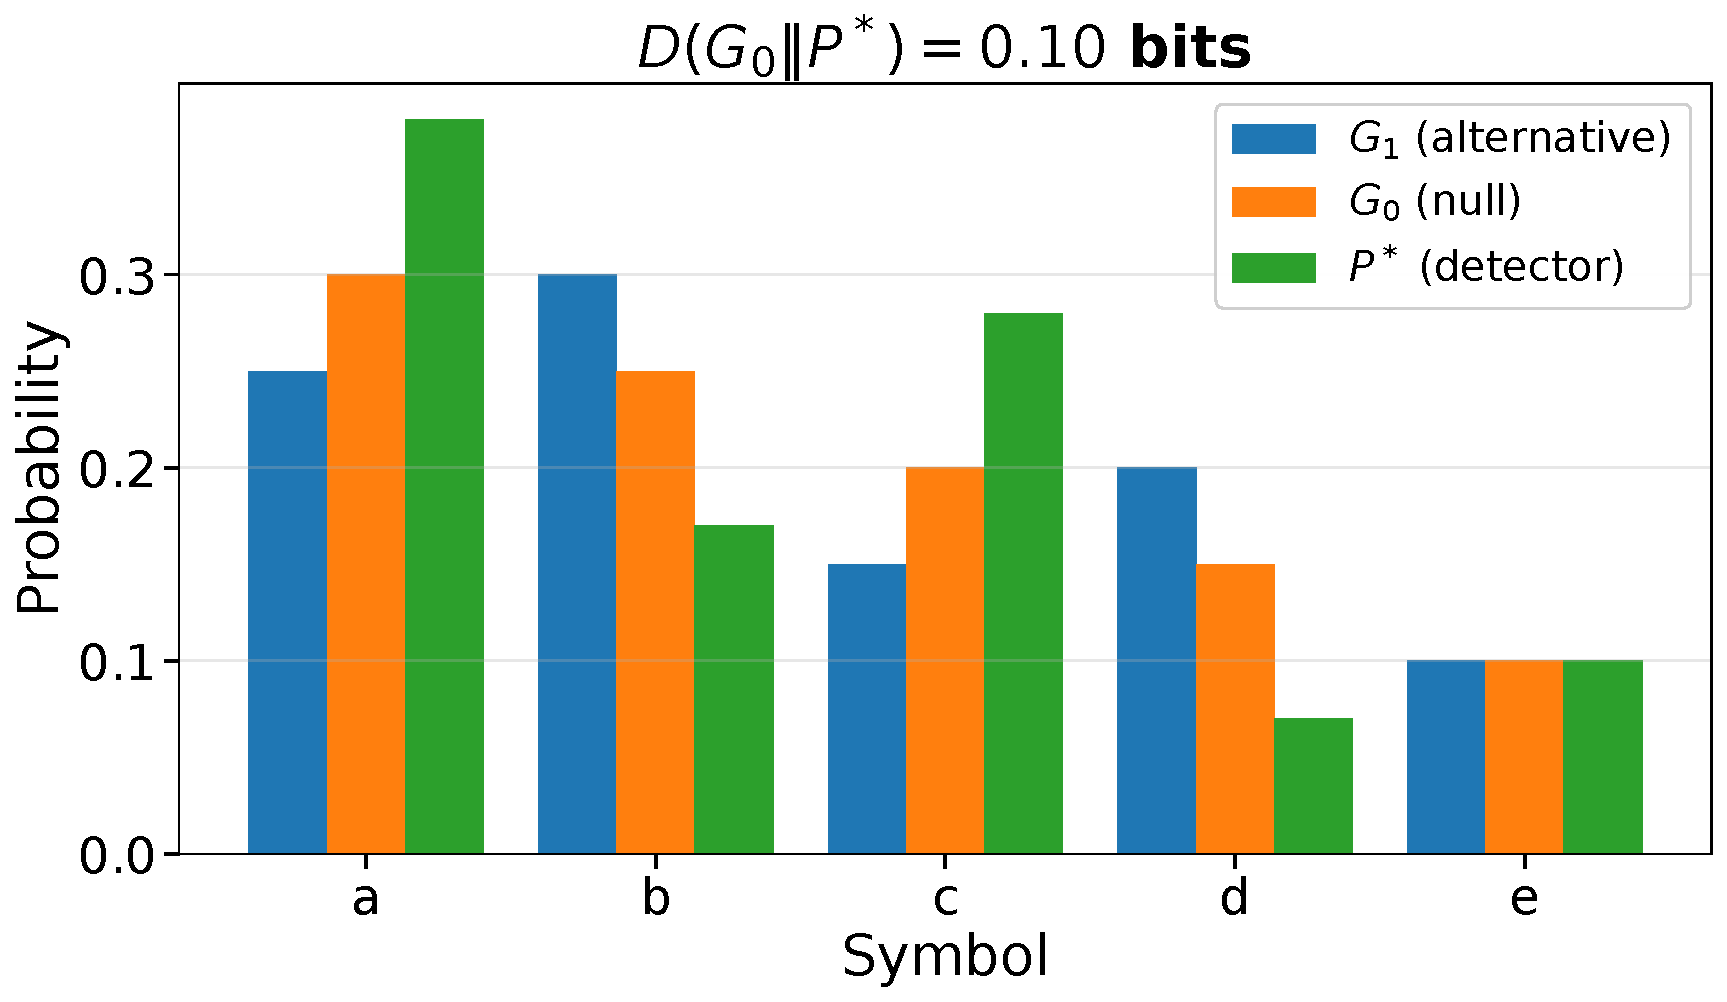
\includegraphics[width=0.80\linewidth, height=0.605\textheight, keepaspectratio]
    {figures/presentation/epsilon_ball_example.pdf}
\end{frame}

\note{
\textbf{Geometry of $P^*$ (Theorem 2).}
\begin{itemize}\small
  \item \textbf{The space is the probability simplex}: $G_0$, $G_1$, $P^*$ are
        each one point = a distribution over the alphabet. $G_1-G_0$ is the
        direction from $G_0$ toward $G_1$; $P^*$ steps the \emph{opposite} way
        (away from $G_1$) along a straight line.
  \item \textbf{Linear}, not geometric/exponential --- the small surprise of
        Thm~2. It subtracts mass from tokens where $G_1$ dominates, raising
        $-\log P$ there.
  \item $\epsilon$ = radius of the KL ball (the budget we choose); in the
        figure $\epsilon = 0.10$ bits --- that is exactly the
        ``$D(G_0\|P^*)=0.10$ bits'' label.
  \item $\gamma$ = step size in the formula; it is NOT free. Eq.~(10),
        $D(G_0\|P^*)=\epsilon$, pins $\gamma$ so $P^*$ lands exactly on the
        ball's boundary (constraint active, since $\Delta$ grows as we move
        away from $G_0$). So $\epsilon$ isn't written in eq.~(9): it enters
        through $\gamma$. Bigger $\epsilon\Rightarrow$ bigger
        $\gamma\Rightarrow P^*$ farther from $G_0$.
  \item \textbf{$\gamma\Leftrightarrow\epsilon$ relation:} no closed form in general
        (solve $\epsilon=-\sum_x G_0\log(1-\gamma\tfrac{G_1-G_0}{G_0})$,
        monotone in $\gamma$). Small-$\epsilon$:
        $\gamma\approx\sqrt{2\epsilon/\Dchi{G_1}{G_0}}$, i.e.
        $\gamma\propto\sqrt\epsilon$. This is the engine behind the
        Thm~3 gain $\sqrt{2\epsilon\,\Dchi{G_1}{G_0}}$.
        ($\epsilon$ in nats; $1/\ln2$ factor if in bits.)
\end{itemize}
}

% ------------------------------------------------------------------
% Frame 9 -- Composite alternatives and self-detection
% ------------------------------------------------------------------
\section{Composite Alternatives}
\begin{frame}[t]{Result 3: When Self-Detection is Locally Maximin-Optimal}
  \vspace{1.2em}
  \begin{columns}[c,onlytextwidth]
    \begin{column}{0.60\textwidth}
      {\small
      \textbf{Single \(G_1\):} move away from \(G_0\).\\[0.25em]
      \textbf{Family of alternatives \(\cG_1\):} optimize the worst case.}

      \[
        \bigDelta^*(\cG_1,G_0)=
        \sup_{P\in\cP_\epsilon(G_0)}\inf_{G\in\cG_1}\bigDelta(G,G_0;P)
      \]

      \vspace{0.5em}
      {\small \textbf{Modeling assumption:} LLM \(G_0\) can be viewed as a learned
      convex mixture of human-style sources:}

      \[
        G_0 \approx \sum_j \pi_j H_j
        \qquad \text{\footnotesize\(\pi_j\ge 0,\ \sum\nolimits_j \pi_j=1\)}
      \]
    \end{column}
    \hfill
    \begin{column}{0.39\textwidth}
      \centering
      \begin{tikzpicture}[scale=1.08]
        \fill[RUBlue] (0,0) circle (3pt)
             node[below=5pt, font=\normalsize]{$G_0$ {\footnotesize(LLM)}};
        \foreach \a in {0,20,...,340} {
          \pgfmathsetmacro{\r}{1.4+0.18*rand}
          \fill[red!50!black, opacity=0.55] (\a:\r) circle (1.8pt);
        }
        \draw[dashed, RUAccent, thick] (0,0) circle (1.6cm);
        \node[black, font=\small, align=center] at (0, -2.35)
             {alternative sources\\[-1pt] around \(G_0\)};
      \end{tikzpicture}
    \end{column}
  \end{columns}

  \vspace{0.15em}
  \begin{callout}[width=0.92\linewidth]
    {\small If alternatives \alert{isotropically surround} \(G_0\):}\\[2pt]
    {\Large \(\boldsymbol{P=G_0}\) is locally maximin optimal}
  \end{callout}
\end{frame}

% ------------------------------------------------------------------
% Frame 10 -- Empirical: normalized log-loss separation predicts AUC
% ------------------------------------------------------------------
\section{Evidence}
\begin{frame}[t]{Empirical Check: Normalized Separation Predicts AUC}
  \begin{columns}[c,onlytextwidth]
    \begin{column}{0.73\textwidth}
      \centering
      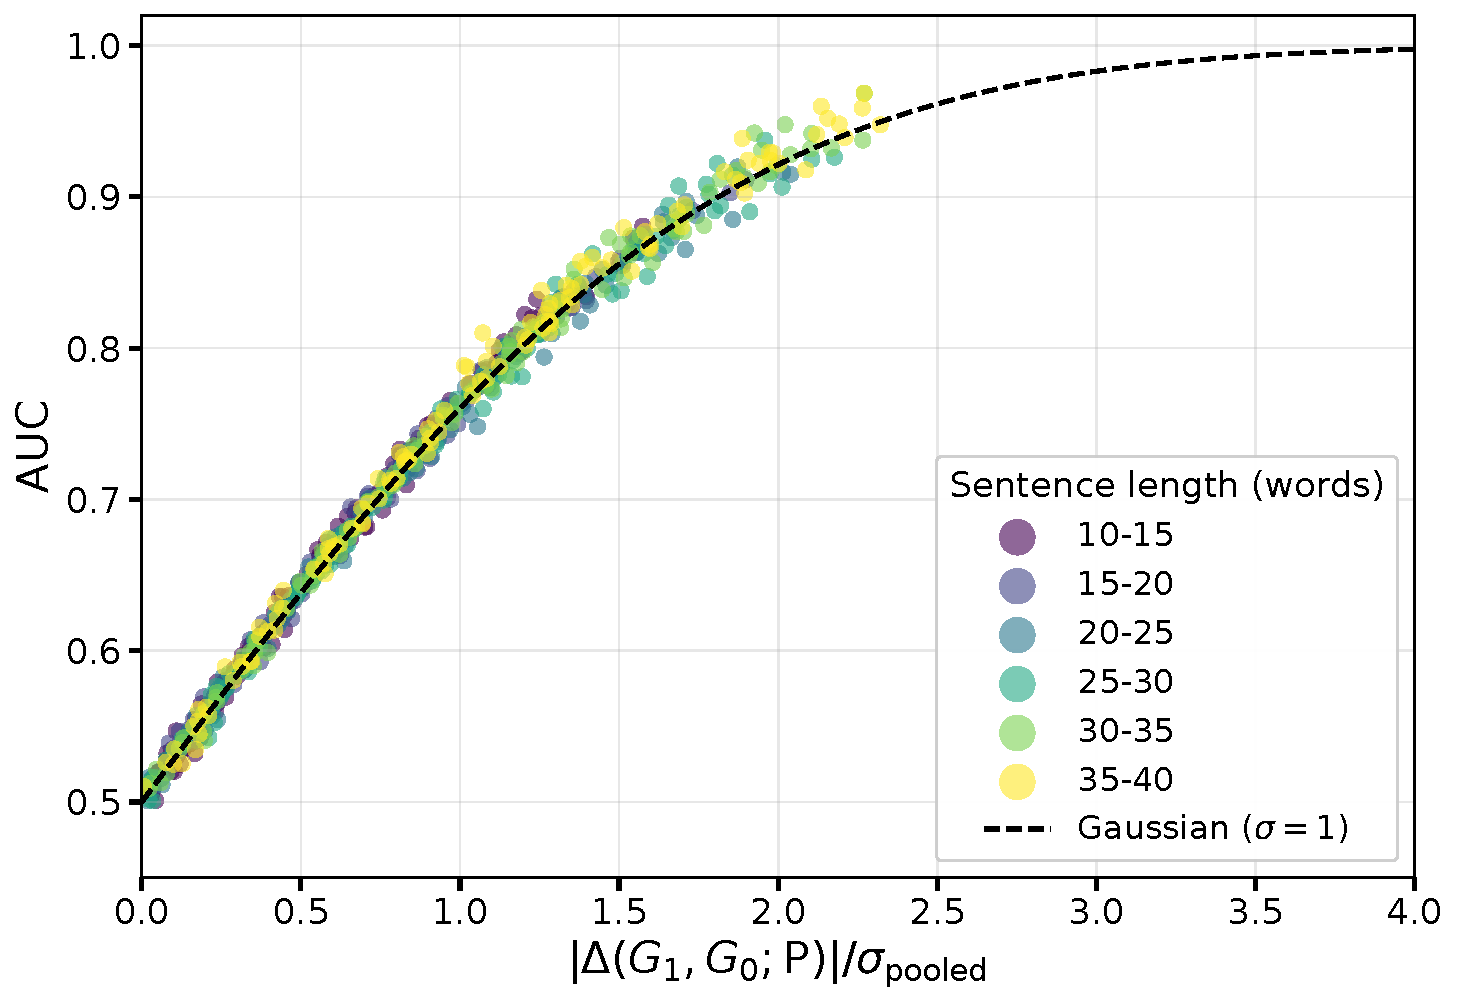
\includegraphics[width=\linewidth, height=0.625\textheight, keepaspectratio]
        {figures/presentation/auc_vs_delta_normalized_unified.pdf}
    \end{column}
    \hfill
    \begin{column}{0.25\textwidth}
      \small\textcolor{black!78}{%
      \(\displaystyle x:=\frac{|\hat\mu_1(P)-\hat\mu_0(P)|}{\hat\sigma_{\mathrm{pooled}}}\)\\[12pt]
      \(\mathrm{AUC}\approx\Phi(x/\sqrt{2})\)}
    \end{column}
  \end{columns}

  \vspace{0.3em}
  {\small \textbf{Experiment setup:} 275,000 sentences, 3 domains, 5 authors, 4 detector models}\\[2pt]
  {\small Empirical AUC follows the Gaussian curve:
  \alert{Pearson \(r=0.99\).}}\\[2pt]
  {\small\textcolor{RUBlue}{\textbf{Supports Result 1:}
  Gaussian-like log-loss behavior and stable variance.}}\\[2pt]
  {\footnotesize\textcolor{black!78}{Max/min standard-deviation ratio
  across detectors is \(1.2\)--\(1.5\times\).}}
\end{frame}

\note{
\textbf{VALIDATION, not a discovery.}
\begin{itemize}\small
  \item Don't pitch ``more separation $\to$ higher AUC'' as a finding ---
        obvious/monotone for any score.
  \item $\Phi(x/\sqrt2)$ = textbook binormal-AUC formula
        ($\mathrm{AUC}=\Pr(S_1>S_0)$ for two equal-variance Gaussians).
        We did NOT compute AUC with it: AUC is measured from the ROC
        (\texttt{roc\_auc\_score}); the curve is just overlaid. Parameter-free.
  \item Three claims tested: (1) $\Delta=D(G_1\|P)-D(G_0\|P)$ governs separation
        (Thm~1, not a priori obvious); (2) the unimodal, variance-stable
        Gaussian model (A1--A2) holds on real text; (3) the link is
        quantitative, not just directional.
  \item $r=0.99$ supports \textbf{A1--A2} (paper attributes Fig.~3 to A1--A2).
        \textbf{A3} ($\sigma$ independent of $P$) is checked \emph{separately}
        by the $1.2$--$1.5\times$ $\sigma$-ratio (Fig.~2). Single-$\sigma$ form
        assumes $\sigma_0\approx\sigma_1$; else
        $\Phi\!\big((\mu_1-\mu_0)/\sqrt{\sigma_0^2+\sigma_1^2}\big)$.
  \item Say: ``AUC measured from the ROC follows the parameter-free $\Phi(x/\sqrt2)$
        almost perfectly, so Thm~1's assumptions hold.'' Contribution = THEORY
        ($\Delta$ governs power; $P=G_0$ can be maximin); plot = credibility check.
\end{itemize}
}

% ------------------------------------------------------------------
% Frame 11 -- Human vs LLM evidence
% ------------------------------------------------------------------
\begin{frame}[t]{LLM vs.\ Human: Support for the Maximin Choice \(P=G_0\)}
  \centering
  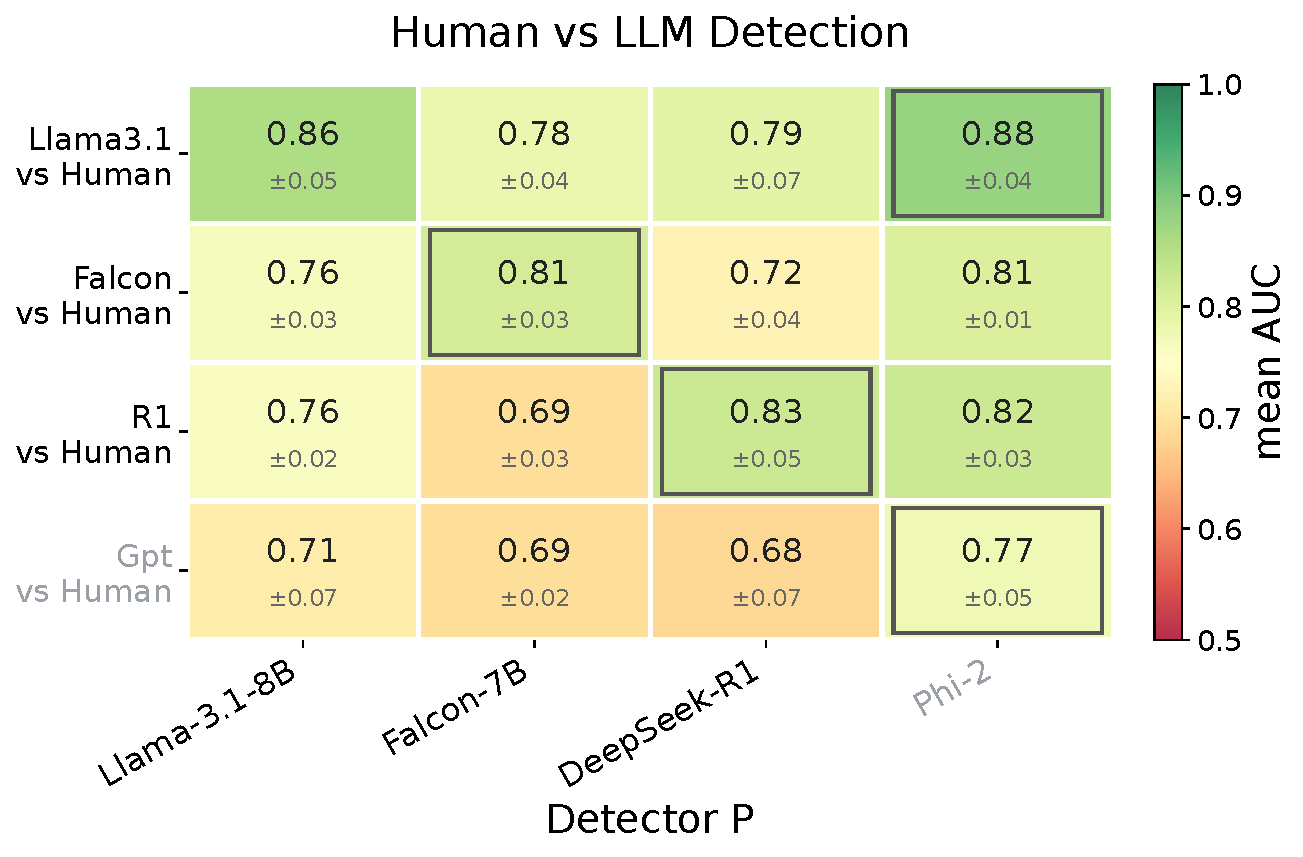
\includegraphics[width=0.98\linewidth, height=0.63\textheight, keepaspectratio]
    {figures/presentation/human_detection_heatmap_avg.pdf}

  \vfill
  \begin{columns}[c,onlytextwidth]
    \begin{column}{0.42\textwidth}
      \small\textbf{Matched detector \(P=G_0\):}
      \begin{itemize}
        \setlength\itemsep{0.1em}
        \item \alert{Best in 4/9} cases, second-best in 5/9
        \item Mean AUC \(\mathbf{0.831}\) vs.\ \(0.626\) for LLM-vs-LLM
      \end{itemize}
    \end{column}
    \hfill
    \begin{column}{0.55\textwidth}
      \begin{callout}[top=4pt,bottom=4pt,before skip=0pt,after skip=0pt,
          colframe=RUBlue!45, boxrule=0.5pt,
          borderline west={3pt}{0pt}{RUAccent}]
        \small Consistent with the maximin model if LLM \(G_0\) is surrounded
        by human sources.
      \end{callout}
    \end{column}
  \end{columns}
\end{frame}

% ------------------------------------------------------------------
% Frame 12 -- Contribution, not recap
% ------------------------------------------------------------------
\section{Takeaway}
\begin{frame}{Takeaway}
  \vfill
  \begin{enumerate}
    \setlength{\itemsep}{2.6em}
    \item When candidate-model likelihoods are unavailable,
          detect with a third model \(P\).

    \item The power-maximizing detector maximizes
          \(\bigDelta(G_1,G_0;P)=\Dkl{G_1}{P}-\Dkl{G_0}{P}\).

    \item For composite alternatives isotropically surrounding \(G_0\),
          self-detection is locally the maximin optimal choice.
  \end{enumerate}
  \vfill
\end{frame}

% ------------------------------------------------------------------
% Frame 13 -- Landing
% ------------------------------------------------------------------
{
\setbeamercolor{background canvas}{bg=RUBlue}
\setbeamercolor{normal text}{fg=white}
\usebeamercolor[fg]{normal text}
\hypersetup{urlcolor=white}
\begin{frame}[plain, c]
  \centering
  {\LARGE\textbf{Choose the detector. Maximize the gap.}}\\[1.8em]
  {\normalsize
    Adam Vinestock \quad\textbullet\quad
    \href{mailto:adam.vinestock@post.runi.ac.il}%
         {\texttt{adam.vinestock@post.runi.ac.il}}\\[3pt]
    Alon Kipnis \quad\textbullet\quad
    \href{mailto:alon.kipnis@runi.ac.il}%
         {\texttt{alon.kipnis@runi.ac.il}}
  }\\[1.4em]
  {\small Extended version \& proofs}\\[2pt]
  {\footnotesize\href{https://cs.idc.ac.il/~kipnis}%
                     {\texttt{cs.idc.ac.il/\~{}kipnis}}}
\end{frame}
}

% =================================================================
% BACKUP / APPENDIX
% =================================================================
\appendix
\metroset{numbering=none, progressbar=none}

% ------------------------------------------------------------------
% Backup B1 -- Theorem 3
% ------------------------------------------------------------------
\begin{frame}{How Sub-Optimal Is \(P=G_0\)?}
  Small-\(\epsilon\) expansion of the optimal gap:
  \[
    \bigDelta(G_1,G_0;P^*)
    =
    \Dkl{G_1}{G_0}
    +\sqrt{2\epsilon\,\Dchi{G_1}{G_0}}
    +O(\epsilon).
  \]

  \medskip
  \begin{callout}
    Deviating from \(G_0\) can raise the gap by
    \(\approx\sqrt{2\epsilon\,\Dchi{G_1}{G_0}}\),
    quantifying the sub-optimality of \(P=G_0\) against a
    \textbf{simple} alternative.
  \end{callout}

  \medskip
  \textbf{Where this comes from: the \(\gamma \Leftrightarrow \epsilon\) relation.}
  The constraint \(D(G_0\|P^*)=\epsilon\) fixes the step size \(\gamma\).
  It has no closed form in general, but for small \(\epsilon\)
  \[
    \epsilon \approx \tfrac{\gamma^2}{2}\,\Dchi{G_1}{G_0}
    \qquad\Longleftrightarrow\qquad
    \gamma \approx \sqrt{\tfrac{2\epsilon}{\Dchi{G_1}{G_0}}}
    \;\;(\gamma\propto\sqrt{\epsilon}),
  \]
  which substituted into the gap produces the
  \(\sqrt{2\epsilon\,\Dchi{G_1}{G_0}}\) term above.

  \medskip
  {\footnotesize Here
  \(\Dchi{G_1}{G_0}=\sum_x (G_1(x)-G_0(x))^2/G_0(x)\);
  \(\epsilon\) in nats (\(1/\ln2\) factor if measured in bits).}
\end{frame}

% ------------------------------------------------------------------
% Backup B2 -- Theorem 4
% ------------------------------------------------------------------
\begin{frame}{The Maximin Mechanism}
  For a composite family \(\cG_1\), the local maximin gap is set by
  a least-favorable prior \(\pi^*\):
  \[
    \bigDelta^*(\cG_1,G_0)
    =
    \mathbb{E}_{G\sim\pi^*}\!\left[\Dkl{G}{G_0}\right]
    +\sqrt{2\epsilon\,\Dchi{\bar G_{\pi^*}}{G_0}}
    +O(\epsilon),
  \]
  \[
    \bar G_{\pi^*}(x)=\mathbb{E}_{G\sim\pi^*}[G(x)].
  \]

  \begin{callout}
    If a non-convex alternative family isotropically surrounds \(G_0\),
    this mechanism yields Corollary 5.1: \(P=G_0\) is locally maximin.
  \end{callout}
\end{frame}

% ------------------------------------------------------------------
% Backup B2b -- Anisotropy index detail (definitions pushed off main slide 8)
% ------------------------------------------------------------------
\begin{frame}{Anisotropy Index and Isotropic Optimality}
  For a prior \(\pi^{\#}\) on \(\cG_1\) with \(G_0=\bar G_{\pi^{\#}}=\mathbb{E}_{G\sim\pi^{\#}}[G]\):
  \[
    \bar D_{\pi^{\#}}=\mathbb{E}_{G\sim\pi^{\#}}\Dkl{G}{G_0},
    \qquad
    r_{\pi^{\#}}=\sup_{G\in\operatorname{supp}(\pi^{\#})}
      \bigl|\Dkl{G}{G_0}-\bar D_{\pi^{\#}}\bigr|.
  \]
  \(r_{\pi^{\#}}=0\) iff all sources are equidistant from \(G_0\) in relative
  entropy (the mixture is isotropic); it grows with the unevenness of those
  distances.

  \medskip
  For any alternative \(G\in\cG_1\), the self-detector \(P=G_0\) obeys
  \[
    \bigDelta(G,G_0;G_0)=\Dkl{G}{G_0}
    \;\ge\;\bigDelta^*(\cG_1,G_0)-r_{\pi^{\#}}+O(\epsilon),
  \]
  so its worst-case sub-optimality is at most \(r_{\pi^{\#}}\). When
  \(r_{\pi^{\#}}=0\),
  \[
    \inf_{G\in\cG_1}\Dkl{G}{G_0}=\bigDelta^*(\cG_1,G_0)+O(\epsilon),
  \]
  i.e.\ \(P=G_0\) is locally maximin optimal.
\end{frame}

% ------------------------------------------------------------------
% Backup B3 -- Experimental setup
% ------------------------------------------------------------------
\begin{frame}{Experimental Setup}
  \begin{columns}[T,onlytextwidth]
    \begin{column}{0.48\textwidth}
      \textbf{Datasets} {\small(3 domains, matched topics)}
      \begin{itemize}
        \setlength\itemsep{0.25em}
        \item Wikipedia, News, Scientific abstracts
        \item \(\sim\!4{,}500\) docs, \(\sim\!275{,}000\) sentences
        \item Sentence length: 10--40 words
        \item Scored without preceding context
      \end{itemize}
    \end{column}
    \hfill
    \begin{column}{0.48\textwidth}
      \textbf{Authors / Detectors}
      \begin{itemize}
        \setlength\itemsep{0.25em}
        \item Authors: Llama-3.1, Falcon, GPT-3.5, DeepSeek-R1, Human
        \item Detectors \(P\): Llama-3.1, Falcon, Phi-2, DeepSeek-R1
        \item Some coincide \(\Rightarrow\) self-detection (\(P=G_0\))
      \end{itemize}
    \end{column}
  \end{columns}

  \vfill
  \begin{callout}
    GPT-3.5 model inaccessible for evaluation, so self-detection
    isn't possible.
  \end{callout}
\end{frame}

% ------------------------------------------------------------------
% Backup B4 -- Length confounding
% ------------------------------------------------------------------
\begin{frame}{Why Normalize?}
  \centering
  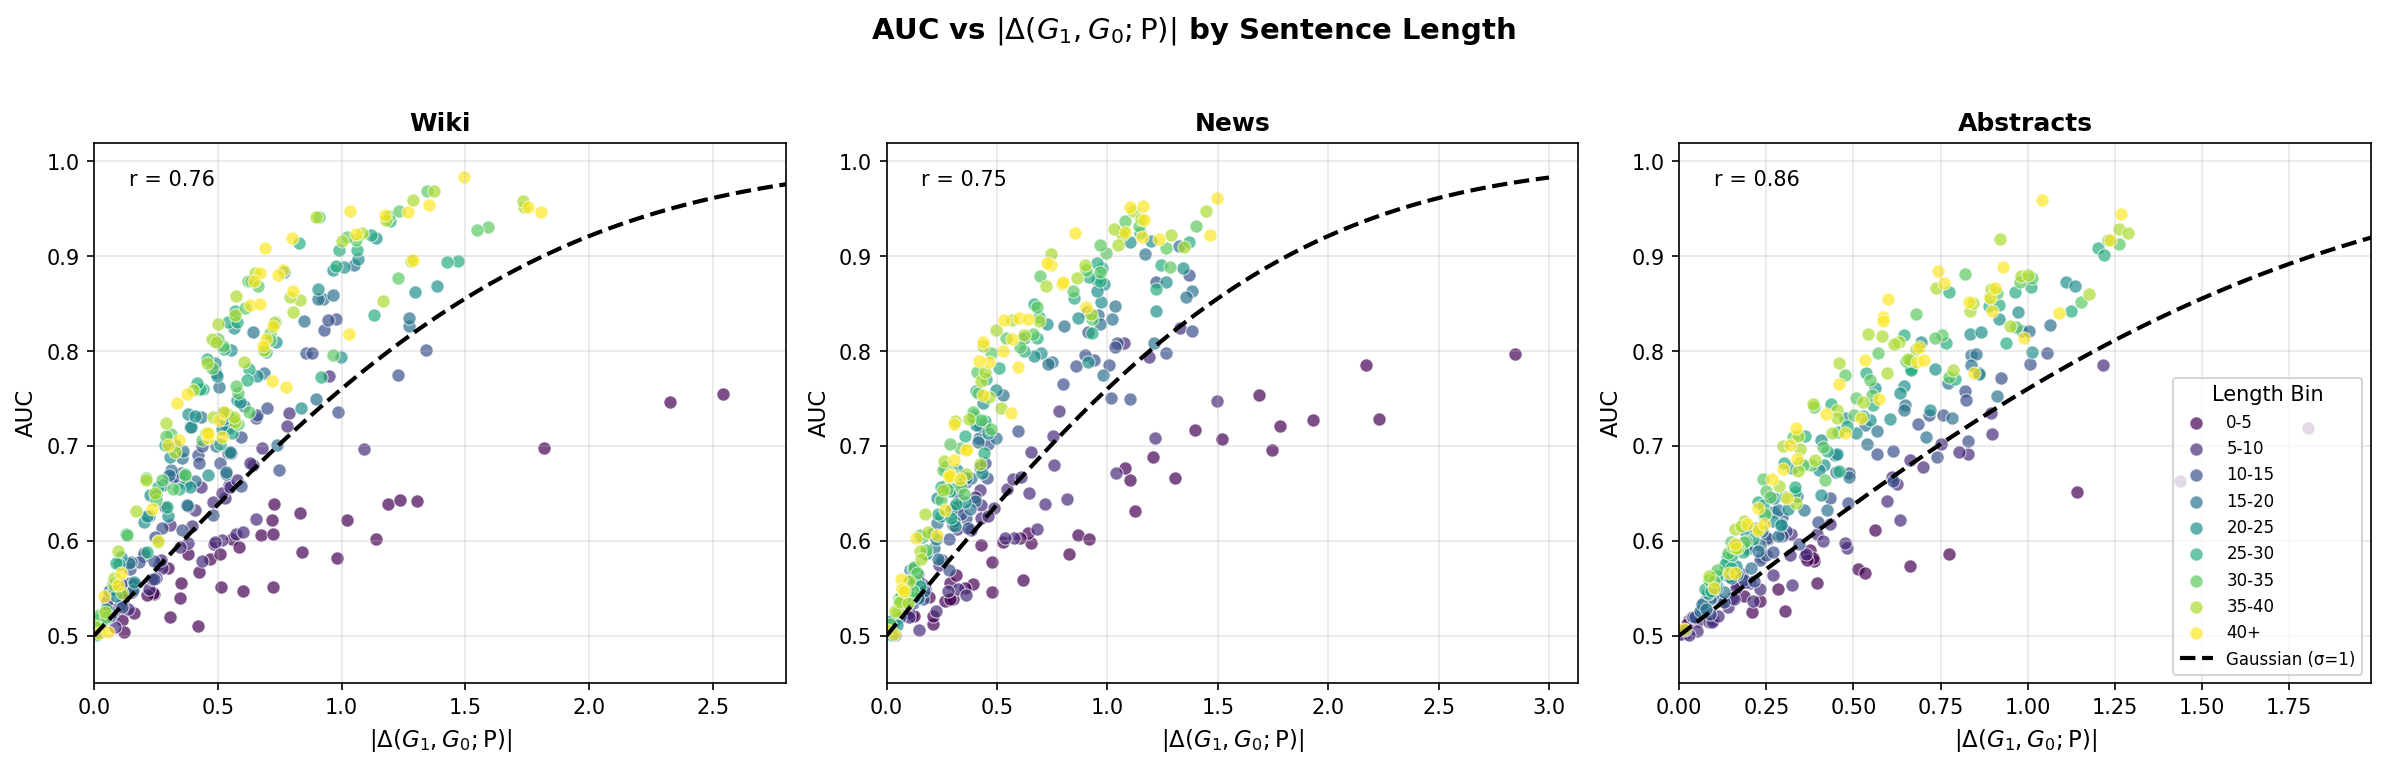
\includegraphics[width=0.95\linewidth, height=0.66\textheight, keepaspectratio]
    {figures/delta_auc_by_length.png}

  \vspace{0.3em}
  {\small Raw log-loss gaps are confounded by length. Dividing by
  \(\hat\sigma_{\mathrm{pooled}}\) collapses length bins onto the
  Gaussian AUC curve used in the main evidence slide.}
\end{frame}

% ------------------------------------------------------------------
% Backup B5 -- Variance stability
% ------------------------------------------------------------------
\begin{frame}{Variance Stability by Length}
  \centering
  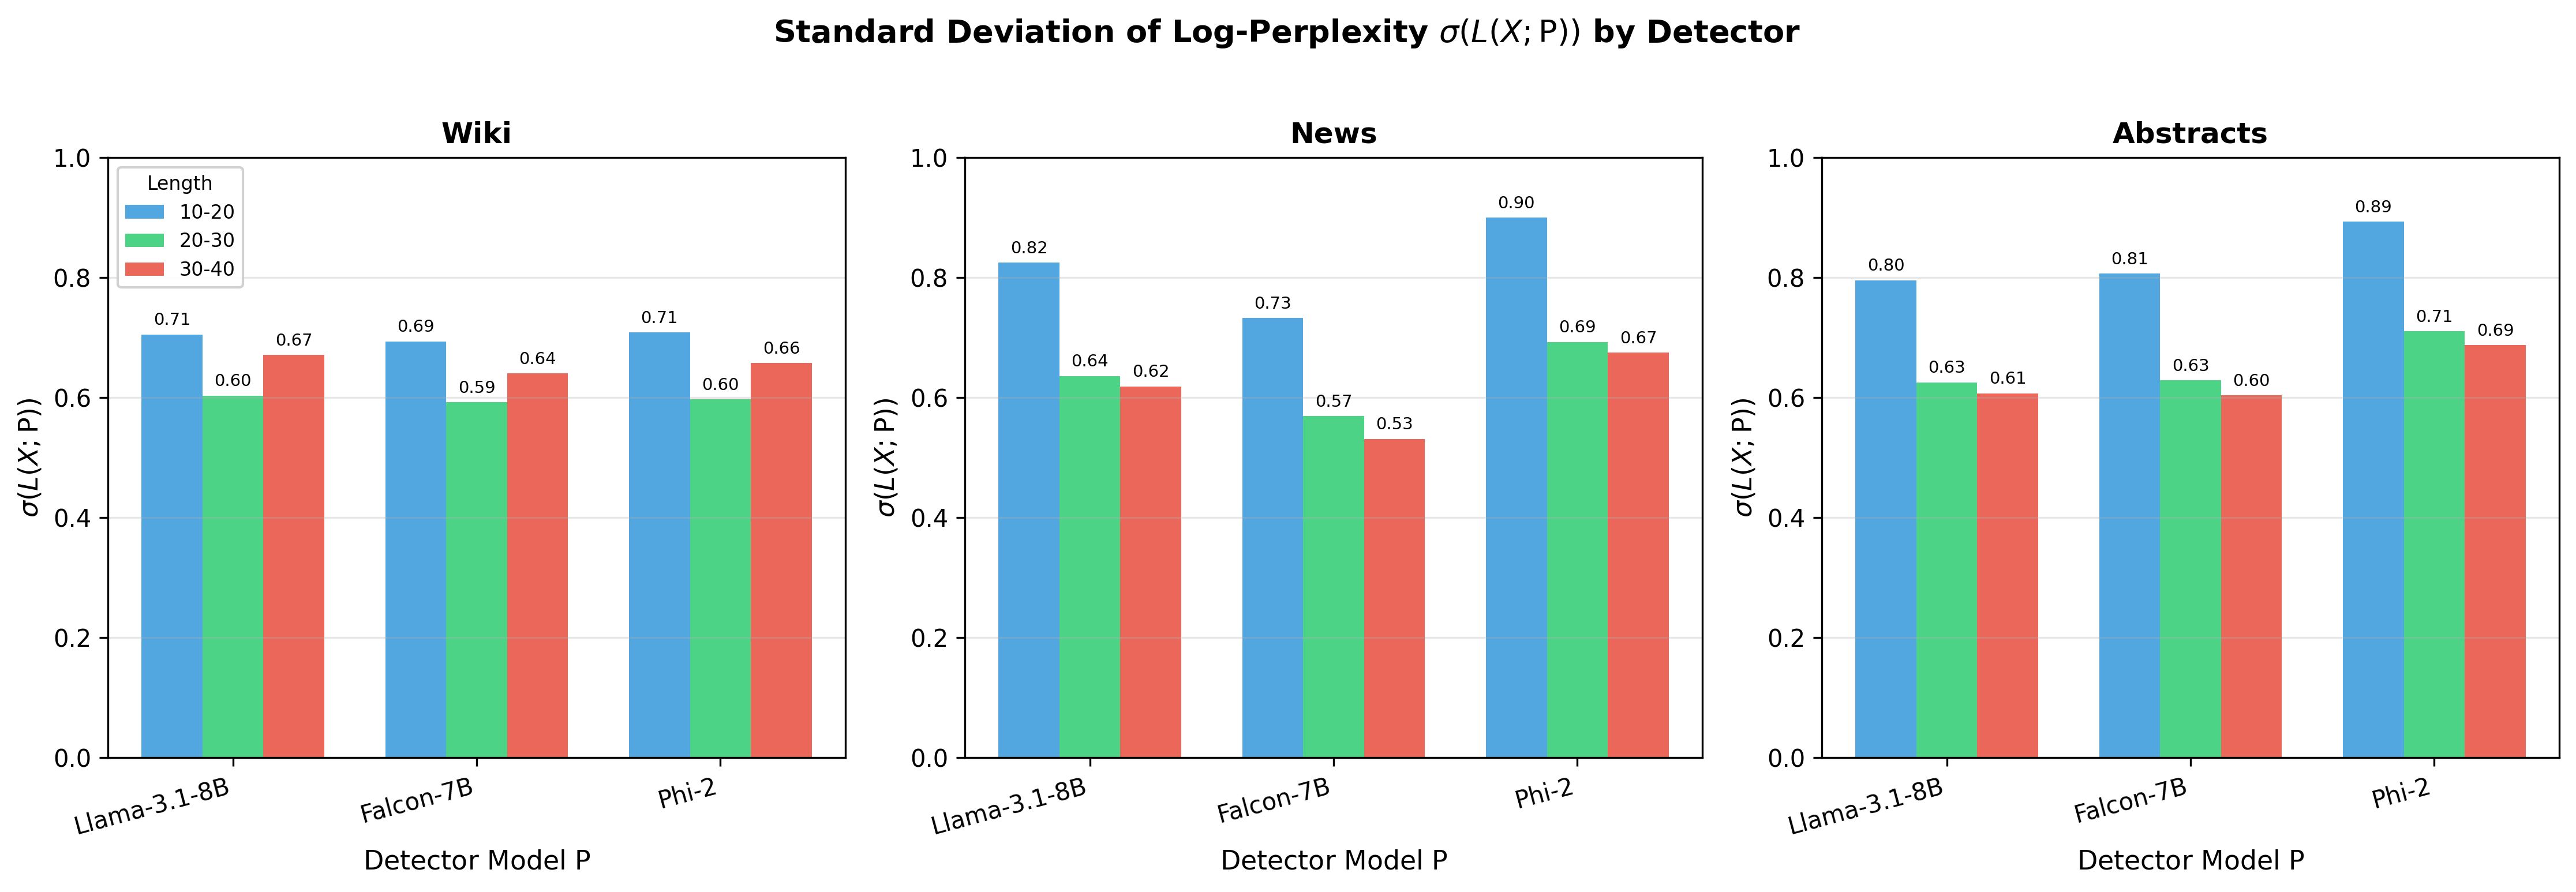
\includegraphics[width=\linewidth, height=0.62\textheight, keepaspectratio]
    {figures/sigma_vs_detector.png}

  \vspace{0.3em}
  {\small A3 view: standard deviation \(\sigma(L(X;P))\) by detector, split by
  sentence length. \emph{Within each length bin}, \(\sigma\) is nearly identical
  across Llama-3.1, Falcon, and Phi-2 (across-detector ratio \(\approx
  1.0\)--\(1.3\times\)), supporting A3; the larger spread within a dataset is
  driven by length, not by \(P\). DeepSeek-R1 is excluded as an outlier (its
  chat template inflates \(\sigma\)).}
\end{frame}

% ------------------------------------------------------------------
% Backup B6 -- Matched-detector counting
% ------------------------------------------------------------------
\begin{frame}{What ``Best in 4/9'' Means}
  \begin{itemize}
    \setlength\itemsep{0.55em}
    \item \textbf{The 9 cases:} 3 domains \(\times\) 3 matched LLM authors
          (Llama-3.1, Falcon, DeepSeek-R1).
    \item \textbf{GPT is excluded:} it has no corresponding open detector.
    \item \textbf{Phi-2 is detector-only:} it can win a heatmap cell, but
          is not part of the matched-detector count.
    \item \textbf{The claim:} among matched-detector cases,
          \(P=G_0\) is best in 4/9 and second-best in the remaining 5/9.
  \end{itemize}
\end{frame}

% ------------------------------------------------------------------
% Backup B7 -- AUC table
% ------------------------------------------------------------------
\begin{frame}{Matched-Detector AUC Numbers}
  \vfill
  \centering
  \textbf{AUC when detector matches source (\(P=G_0\))}

  \vspace{0.8em}
  \begin{tabular}{@{}lccc@{}}
    \toprule
    Dataset & Human vs.\ \(G_0\) & \(G_0\) vs.\ \(G_1\) & Gap \\
    \midrule
    Wiki      & \(0.853 \pm 0.006\) & \(0.659 \pm 0.065\) & \(+0.194\) \\
    News      & \(0.854 \pm 0.047\) & \(0.626 \pm 0.094\) & \(+0.229\) \\
    Abstracts & \(0.787 \pm 0.018\) & \(0.592 \pm 0.013\) & \(+0.195\) \\
    \midrule
    \textbf{Mean} & \(\mathbf{0.831}\) & \(\mathbf{0.626}\)
                  & \(\mathbf{+0.206}\) \\
    \bottomrule
  \end{tabular}

  \vspace{0.8em}
  {\small Human-vs-LLM self-detection is substantially easier than
  LLM-vs-LLM matched detection in this experiment.}
  \vfill
\end{frame}

% ------------------------------------------------------------------
% Backup B8--B10 -- Original (paper) versions of the updated plots
% ------------------------------------------------------------------
\begin{frame}{Backup: Original \(P^*\) Example (paper figure)}
  \centering
  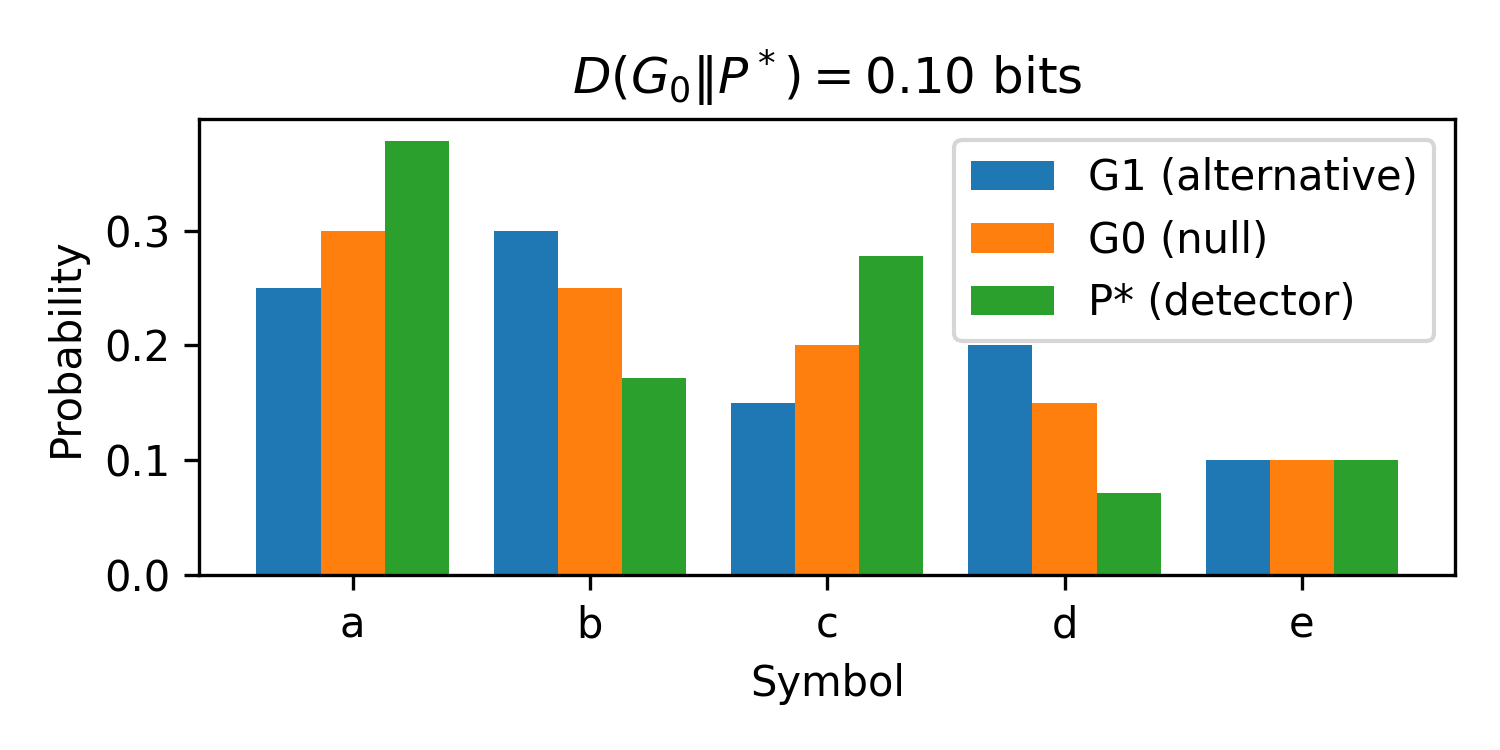
\includegraphics[width=0.92\linewidth, height=0.74\textheight, keepaspectratio]
    {figures/epsilon_ball_example.png}
\end{frame}

\begin{frame}{Backup: Original AUC vs Normalized Separation (paper figure)}
  \centering
  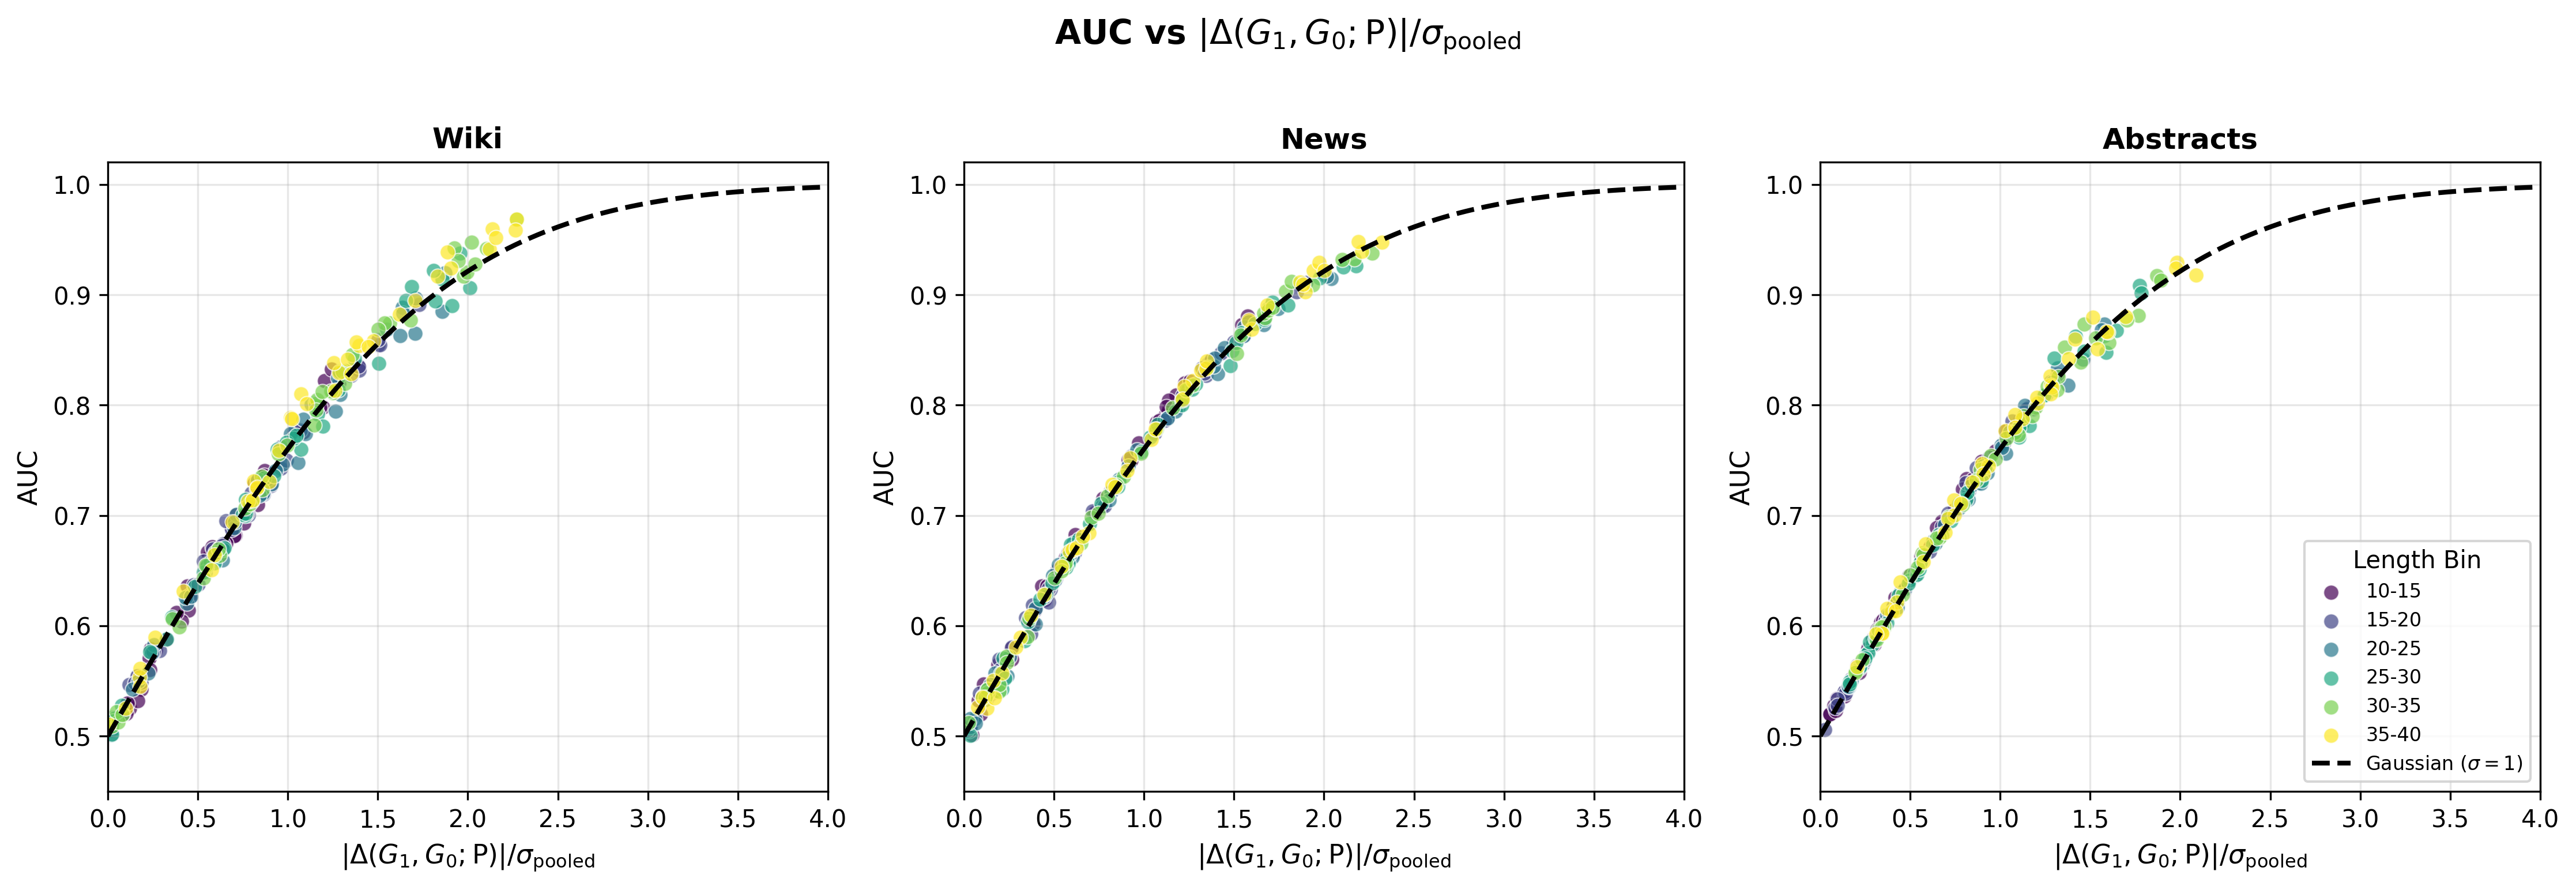
\includegraphics[width=0.96\linewidth, height=0.78\textheight, keepaspectratio]
    {figures/auc_vs_delta_normalized.png}
\end{frame}

\begin{frame}{Backup: Original Human-vs-LLM Heatmap (paper figure)}
  \centering
  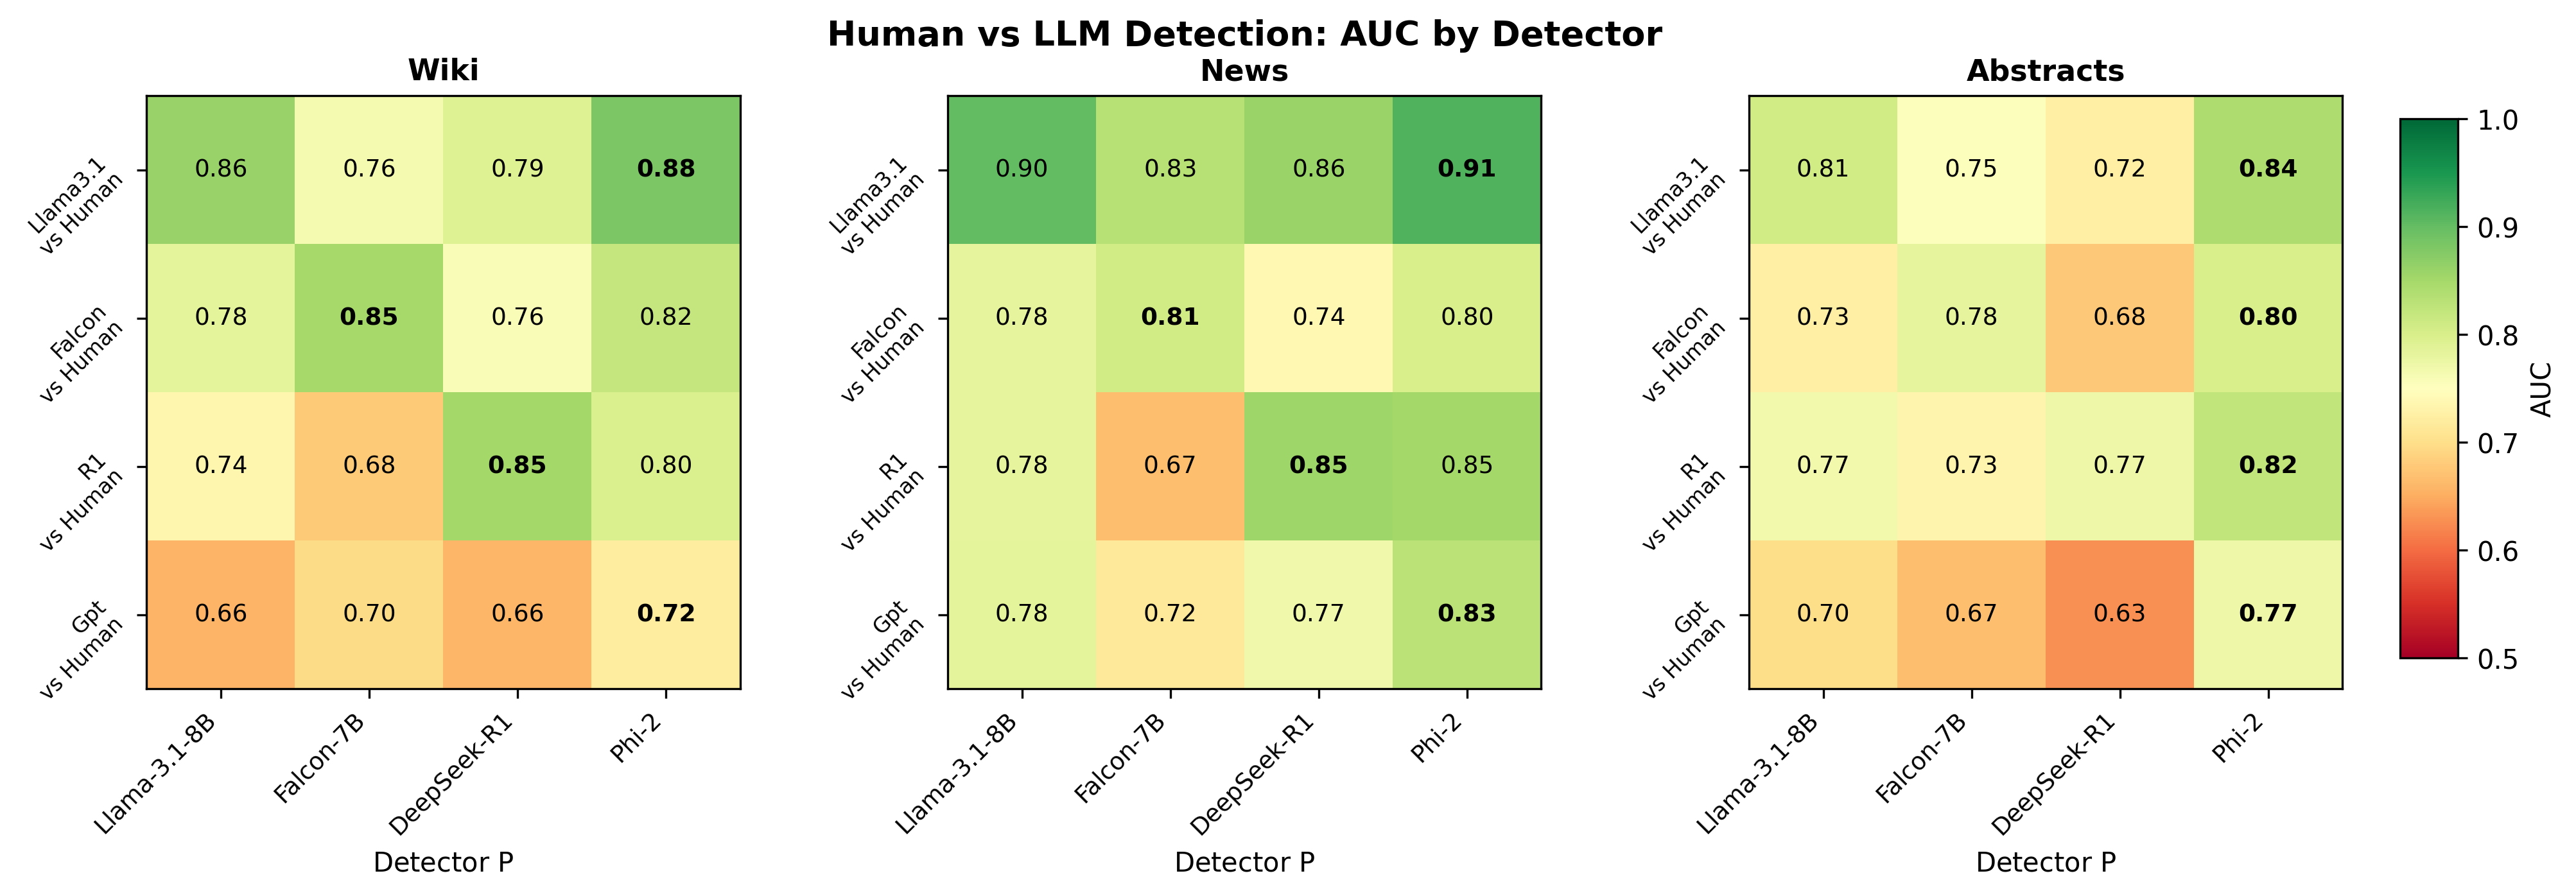
\includegraphics[width=0.96\linewidth, height=0.78\textheight, keepaspectratio]
    {figures/human_detection_heatmap.png}
\end{frame}

\end{document}
"
%   -> renders each slide with its speaker notes on the right (main_with_notes.pdf).
\providecommand{\WithNotes}{0}
\if\WithNotes1
  \usepackage{pgfpages}
  \setbeameroption{show notes on second screen=right}
\fi

% ---------- colours ----------
\definecolor{RUBlue}{RGB}{0, 74, 124}
\definecolor{RUAccent}{RGB}{0, 128, 180}
\definecolor{RUSoft}{RGB}{232, 241, 247}
\definecolor{RUInk}{RGB}{42, 53, 63}
\definecolor{LightGray}{RGB}{245, 245, 245}

\setbeamercolor{frametitle}{bg=RUBlue}
\setbeamercolor{progress bar}{fg=RUAccent}
\setbeamercolor{title separator}{fg=RUAccent}
\setbeamercolor{alerted text}{fg=RUAccent}
\setbeamercolor{normal text}{fg=RUInk}

% ---------- packages ----------
\usepackage{microtype}
\usepackage{amsmath, amssymb, mathtools}
\usepackage{graphicx}
\usepackage{booktabs}
\usepackage{tikz}
\usepackage{appendixnumberbeamer}
\usepackage[most]{tcolorbox}
\usetikzlibrary{arrows.meta, positioning, decorations.pathreplacing, calc, shapes.geometric}

% ---------- hyperref (configure existing beamer-loaded hyperref) ----------
\hypersetup{
  colorlinks=true,
  linkcolor=RUAccent,
  urlcolor=RUAccent,
  citecolor=RUAccent,
  pdftitle={Optimal Log-Likelihood Tests for Distinguishing Generative Models under Relative Entropy Constraints},
  pdfauthor={Adam Vinestock and Alon Kipnis},
}

% ---------- unified callout box ----------
\newtcolorbox{callout}[1][]{
  enhanced,
  colback=RUSoft,
  colframe=RUSoft,
  borderline west={2.4pt}{0pt}{RUAccent},
  boxrule=0pt,
  arc=2pt, outer arc=2pt,
  left=12pt, right=10pt, top=5pt, bottom=5pt,
  before skip=4pt, after skip=4pt,
  fontupper=\centering,
  width=\linewidth,
  #1
}

% ---------- thesis line ----------
\newcommand{\thesisline}[1]{%
  \begin{center}\large\color{RUAccent}#1\end{center}%
}

% ---------- macros ----------
\newcommand{\KL}[2]{D\!\left(#1 \,\middle\|\, #2\right)}
\newcommand{\Dkl}[2]{D(#1 \| #2)}
\newcommand{\Dchi}[2]{D_{\chi^2}(#1 \| #2)}
\newcommand{\bigDelta}{\Delta}
\newcommand{\cP}{\mathcal{P}}
\newcommand{\cG}{\mathcal{G}}
\newcommand{\cX}{\mathcal{X}}
\DeclareMathOperator*{\argmax}{arg\,max}
\DeclareMathOperator*{\argmin}{arg\,min}

% ---------- slide footer logos ----------
% Toggle: set to 0 (or comment out the \ifnum block below) to disable instantly.
\providecommand{\ShowSlideLogos}{1}
\newcommand{\SlideLogoHeight}{0.058\textheight}
\newcommand{\SlideLogoSepX}{1.4em}
\newcommand{\SlideLogoFootSep}{1.1ex}
\newcommand{\SlideLogoReichman}{figures/presentation/footer_reichman_logo.png}
\newcommand{\SlideLogoISIT}{figures/presentation/footer_isit_logo.png}
\ifnum\ShowSlideLogos=1
\setbeamertemplate{footline}{%
  \begin{beamercolorbox}[%
      wd=\paperwidth,%
      sep=\SlideLogoFootSep,%
      leftskip=\SlideLogoSepX,%
      rightskip=\SlideLogoSepX,%
    ]{footline}%
    \begin{minipage}[b]{0.28\paperwidth}%
      \raggedright
      \includegraphics[height=\SlideLogoHeight, keepaspectratio]{\SlideLogoReichman}%
    \end{minipage}%
    \hfill
    \begin{minipage}[b]{0.28\paperwidth}%
      \centering
      \usebeamerfont{page number in head/foot}%
      \usebeamertemplate*{frame numbering}%
    \end{minipage}%
    \hfill
    \begin{minipage}[b]{0.28\paperwidth}%
      \raggedleft
      \includegraphics[height=\SlideLogoHeight, keepaspectratio]{\SlideLogoISIT}%
    \end{minipage}%
  \end{beamercolorbox}%
}
% Logos only (no page number) for plain title/landing-style frames.
\newcommand{\SlideLogosOnly}{%
  \begin{tikzpicture}[remember picture, overlay]
    \node[anchor=south west, inner sep=0,
          xshift=\SlideLogoSepX, yshift=\SlideLogoFootSep]
      at (current page.south west) {%
        \includegraphics[height=\SlideLogoHeight, keepaspectratio]%
          {\SlideLogoReichman}%
    };
    \node[anchor=south east, inner sep=0,
          xshift=-\SlideLogoSepX, yshift=\SlideLogoFootSep]
      at (current page.south east) {%
        \includegraphics[height=\SlideLogoHeight, keepaspectratio]%
          {\SlideLogoISIT}%
    };
  \end{tikzpicture}%
}
\else
\newcommand{\SlideLogosOnly}{}
\fi

% ---------- metadata ----------
\title{Optimal Log-Likelihood Tests for Distinguishing\\
       Generative Models under Relative Entropy Constraints}
\subtitle{How to choose the detector model when the true source is out of reach}
\author{Adam Vinestock \and Alon Kipnis}
\institute{Reichman University, Herzliya, Israel}
\date{ISIT 2026}

% =================================================================
\begin{document}

% ------------------------------------------------------------------
% Frame 1 -- Title / promise
% ------------------------------------------------------------------
\begin{frame}[plain]
  \titlepage
  \SlideLogosOnly
\end{frame}

% ------------------------------------------------------------------
% Frame 2 -- Motivation: oracle unavailable, so a log-loss detector appears
% ------------------------------------------------------------------
\section{Motivation}
\begin{frame}{Testing When Model Likelihoods Are Inaccessible}
  \begin{columns}[c,onlytextwidth]
    \begin{column}{0.62\textwidth}
      \small
      \begin{itemize}
        \setlength\itemsep{0.5em}
        \item Was text \(X\) generated by \(G_0\), or by \(G_1\)?
        \item \textbf{Oracle test:} threshold the likelihood ratio
              \(\log \tfrac{G_1(x)}{G_0(x)}\).
        \item \textbf{Problem:} we can often \emph{sample}, not evaluate
              likelihoods (closed source, compute heavy, inaccessible).
        \item \textbf{Practical test:}
              evaluate logarithmic loss
              \(L(X;P)=\log \tfrac{1}{P(X)}\)
              under a third detector model \(P\)
              {\small(aka perplexity test).}
      \end{itemize}
    \end{column}
    \begin{column}{0.34\textwidth}
      \centering
      \hspace{0.45cm}%
      \begin{tikzpicture}[
          box/.style={
            rounded corners=2pt,
            draw=RUBlue,
            very thick,
            align=center,
            minimum width=3.4cm,
            minimum height=0.82cm,
            fill=RUSoft
          },
          arrow/.style={-{Latex[length=2.2mm]}, very thick, RUAccent}
        ]
        \node[box] (oracle) {oracle LR\\[-1pt]\(\log(G_1/G_0)\)};
        \node[box, below=0.55cm of oracle] (closed) {likelihoods\\unavailable};
        \node[box, below=0.55cm of closed] (detector) {evaluate\\\(L(X;P)\)};
        \draw[arrow] (oracle) -- (closed);
        \draw[arrow] (closed) -- (detector);
      \end{tikzpicture}
    \end{column}
  \end{columns}

  \vfill
  \vspace{0.25em}
  \begin{callout}
    \textbf{Goal: which detector \(P\) maximizes detection power?}\\[-1pt]
    {\small selected by an optimality criterion, not learned inside the test}
  \end{callout}
\end{frame}

% ------------------------------------------------------------------
% Frame 3 (merged) -- Example: empirical log-loss histograms + cites + thesis line.
% The former standalone formula frame is merged here; L(X;P) is now defined on Frame 2.
% Callout dropped; "The goal is maximum separation." kept.
% ------------------------------------------------------------------
\section{Detector}
\begin{frame}{Example: Log-Loss from Two Sources}
  \centering
  {\small Wikipedia sentences from two authors:
  \textbf{Falcon-7B} vs \textbf{Human}, under a third model \(P=\) \textbf{Phi-2}.}

  \vspace{0.1em}
  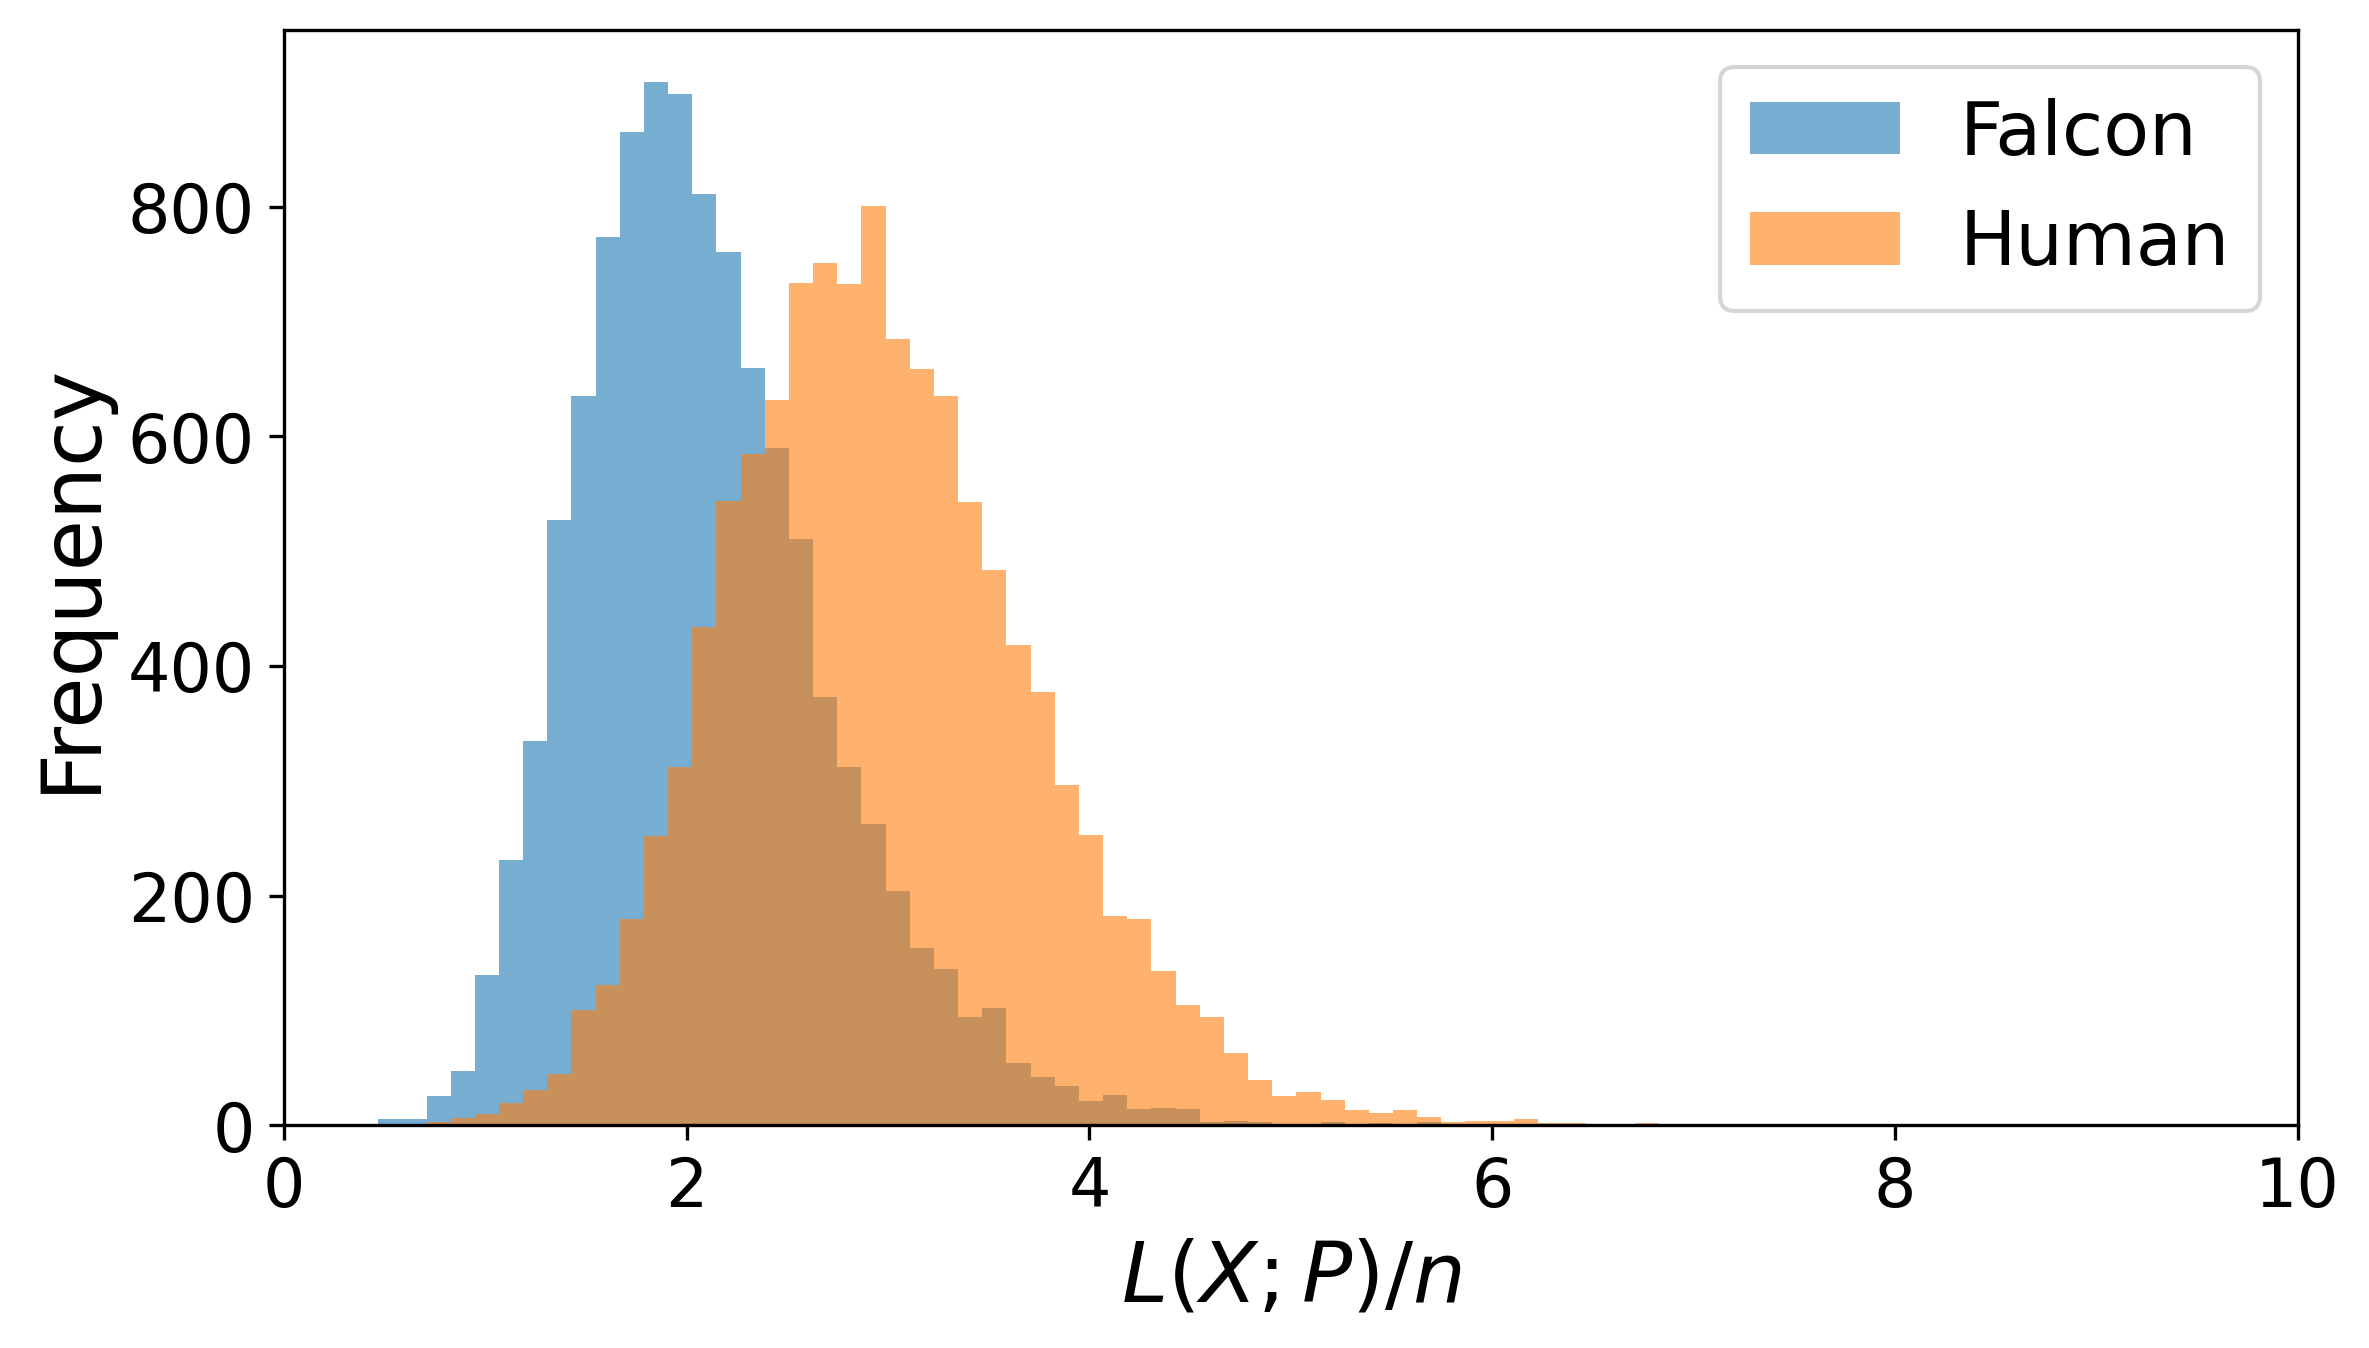
\includegraphics[width=\linewidth, height=0.57\textheight, keepaspectratio]
    {figures/presentation/response_hist_example_v2.png}

  \vspace{0.05em}
  {\scriptsize Related detectors: GLTR (Gehrmann et al., 2019),
   HowKGPT (Vasilatos et al., 2023), Binoculars (Hans et al., 2024).}

  \thesisline{The goal is maximum separation}
\end{frame}

% ------------------------------------------------------------------
% Frame 5 -- Related work
% ------------------------------------------------------------------
\begin{frame}{Related Work}
  \small
  \vfill
  Prior work addresses \textbf{adjacent problems} but not this
  \textbf{detector selection optimality question}:
  \vfill

  \begin{itemize}
    \setlength\itemsep{1.4em}

    \item \textbf{Unconstrained optimal detection} -
    Neyman-Pearson; Lehmann-Romano (2006)\\[-1pt]
    {\footnotesize When both models are known, thresholding the likelihood ratio
    \(\frac{G_1(X)}{G_0(X)}\) is optimal.}

    \item \textbf{Mismatched divergence} -
    Unnikrishnan, Huang, Meyn, Surana \& Veeravalli (2011)\\[-1pt]
    {\footnotesize Studies hypothesis testing when the ideal KL-based statistic
    is replaced by a mismatched one.}

    \item \textbf{M-projection / reverse I-projection} -
    Amari \& Nagaoka (2000)\\[-1pt]
    {\footnotesize Studies KL-based projection geometry over probability
    distributions; related to our objective, which is linear in
    \(\log p\).}

  \end{itemize}
  \vfill
\end{frame}

\note{
The oracle benchmark is Neyman-Pearson. Related work has studied
mismatched test statistics and KL projection geometry. Our work uses
this neighborhood of ideas, but applies it to choosing the detector model for
log-loss testing.
}

% ------------------------------------------------------------------
% Frame 6 -- Formal setup
% ------------------------------------------------------------------
\section{Setup}
\begin{frame}{Problem Setup}
  \begin{columns}[T,onlytextwidth]
    \begin{column}{0.60\textwidth}
      \textbf{Object:}\;
      \(X\) is the data sequence to attribute.

      \medskip
      \textbf{Hypothesis test:}
      \[
        H_0: X \sim G_0
        \qquad\text{vs.}\qquad
        H_1: X \sim G_1
      \]

      \textbf{Test statistic:}\;
      \(L(X;P) := \log \dfrac{1}{P(X)}\)

      \smallskip
      \textbf{Modeling assumption:}\; \(P\) lies near \(G_0\)
      {\small(shared tokenizer / architecture / training):}
      \[
        \boxed{P \in \cP_\epsilon(G_0)
               = \bigl\{P' : \Dkl{G_0}{P'} \leq \epsilon\bigr\}}
      \]

      {\small\textbf{Constrained optimality:}\; among detectors in this ball,
      we search for the one with maximum detection power.}
    \end{column}
    \hfill
    \begin{column}{0.36\textwidth}
      \centering
      \vspace{0.6em}
      \begin{tikzpicture}[scale=1.00]
        \shade[inner color=white, outer color=RUSoft]
              (0,0) circle (1.55cm);
        \draw[ultra thick, RUBlue] (0,0) circle (1.55cm);
        \node[RUBlue, font=\normalsize] at (0, 2.35)
             {\(\Dkl{G_0}{P}\!\leq\!\epsilon\)};
        \fill[RUBlue]   (0,0)      circle (2.5pt)
             node[below=5pt, font=\Large\bfseries]{\(G_0\)};
        \fill[orange!80!black] (2.55,1.3) circle (2.5pt)
             node[above right=-1pt, font=\large\bfseries]{\(G_1\)};
        \node[orange!80!black, font=\scriptsize, align=center] at (2.72,0.78)
             {alternative\\source};
        \fill[RUAccent] (0.65,0.82)  circle (2.5pt)
             node[right=3pt, font=\large\bfseries]{\(P\)};
        \fill[RUAccent] (-0.55,0.42) circle (2.5pt)
             node[left=3pt,  font=\large\bfseries]{\(P'\)};
        \fill[RUAccent] (0.35,-0.82) circle (2.5pt)
             node[right=3pt, font=\large\bfseries]{\(P''\)};
      \end{tikzpicture}
    \end{column}
  \end{columns}
\end{frame}

% ------------------------------------------------------------------
% Frame 7 -- Theorem 1: Delta controls power
% ------------------------------------------------------------------
\section{Main Result}
\begin{frame}{Result 1: Detector Power is Governed by \(\bigDelta\)}
  \small
  \textbf{Assumptions:} under \(G_0\) and \(G_1\), normalized log-loss is unimodal
  with variance stable across detectors.

  Power is monotone in the separation between the two log-loss distributions:
  \vspace{-0.25em}
  \[
    \mu_1(P)-\mu_0(P)
    =
    \underbrace{H(G_1)-H(G_0)}_{\text{fixed}}
    +
    \underbrace{\bigDelta(G_1,G_0;P)}_{\text{depends on }P}
  \]
  \vspace{-0.8em}
  {\Large
  \[
    \boxed{\bigDelta(G_1,G_0;P)
    :=\Dkl{G_1}{P}-\Dkl{G_0}{P}}
  \]
  }
  \vspace{-0.55em}

  \centering
  \begin{tikzpicture}[
      declare function={
        gauss(\x,\m,\s)=exp(-(\x-\m)^2/(2*\s^2))/(\s*sqrt(2*pi));
      }
    ]
    \begin{scope}[xscale=1.22, yscale=2.45]
      \draw[->, thick] (-3,0) -- (6.5,0)
           node[right, font=\footnotesize]{\(L(X;P)/n\)};
      \draw[RUBlue, very thick, domain=-3:3.8, samples=80]
           plot (\x, {gauss(\x,0,1)});
      \draw[red!70!black, very thick, domain=-0.8:6.5, samples=80]
           plot (\x, {gauss(\x,2.8,1)});
      \node[RUBlue, font=\small] at (0, 0.46)
           {\(\mu_0(P)\)};
      \node[red!70!black, font=\small] at (2.8, 0.46)
           {\(\mu_1(P)\)};
      \draw[<->, very thick, RUAccent]
           (0, -0.07) -- node[below, font=\small]
           {controlled by \(\bigDelta\)} (2.8, -0.07);
      \node[gray, font=\scriptsize, align=center] at (5.25, 0.32)
           {\(\sigma \approx\) stable\\[-1pt] across \(P\)};
    \end{scope}
  \end{tikzpicture}

  \vspace{-0.1em}
  \thesisline{Theorem~1: maximizing \(\bigDelta\) maximizes power at fixed Type-I level.}
\end{frame}

% ------------------------------------------------------------------
% Frame 8 -- Theorem 2: optimal detector for a simple alternative
% ------------------------------------------------------------------
\begin{frame}[t]{Result 2: Choosing the Optimal Detector \(P^*\)}
  \[
    \boxed{\vcenter{\hbox{$\displaystyle \max_{P \in \cP_\epsilon(G_0)}\;\bigDelta(G_1,G_0;P)$}}}
    \qquad\Longrightarrow\qquad
    \boxed{\vcenter{\hbox{$\displaystyle P^*(x)=G_0(x)-\gamma\bigl(G_1(x)-G_0(x)\bigr)$}}}
  \]
  \vspace{-0.3em}
  {\small\centering
  \textbf{Theorem 2:} \(P^*\) moves \alert{linearly away} from \(G_0\),
  opposite to \(G_1\), with \(D(G_0\|P^*)=\epsilon\).\par}

  \vspace{1.1em}
  \centering
  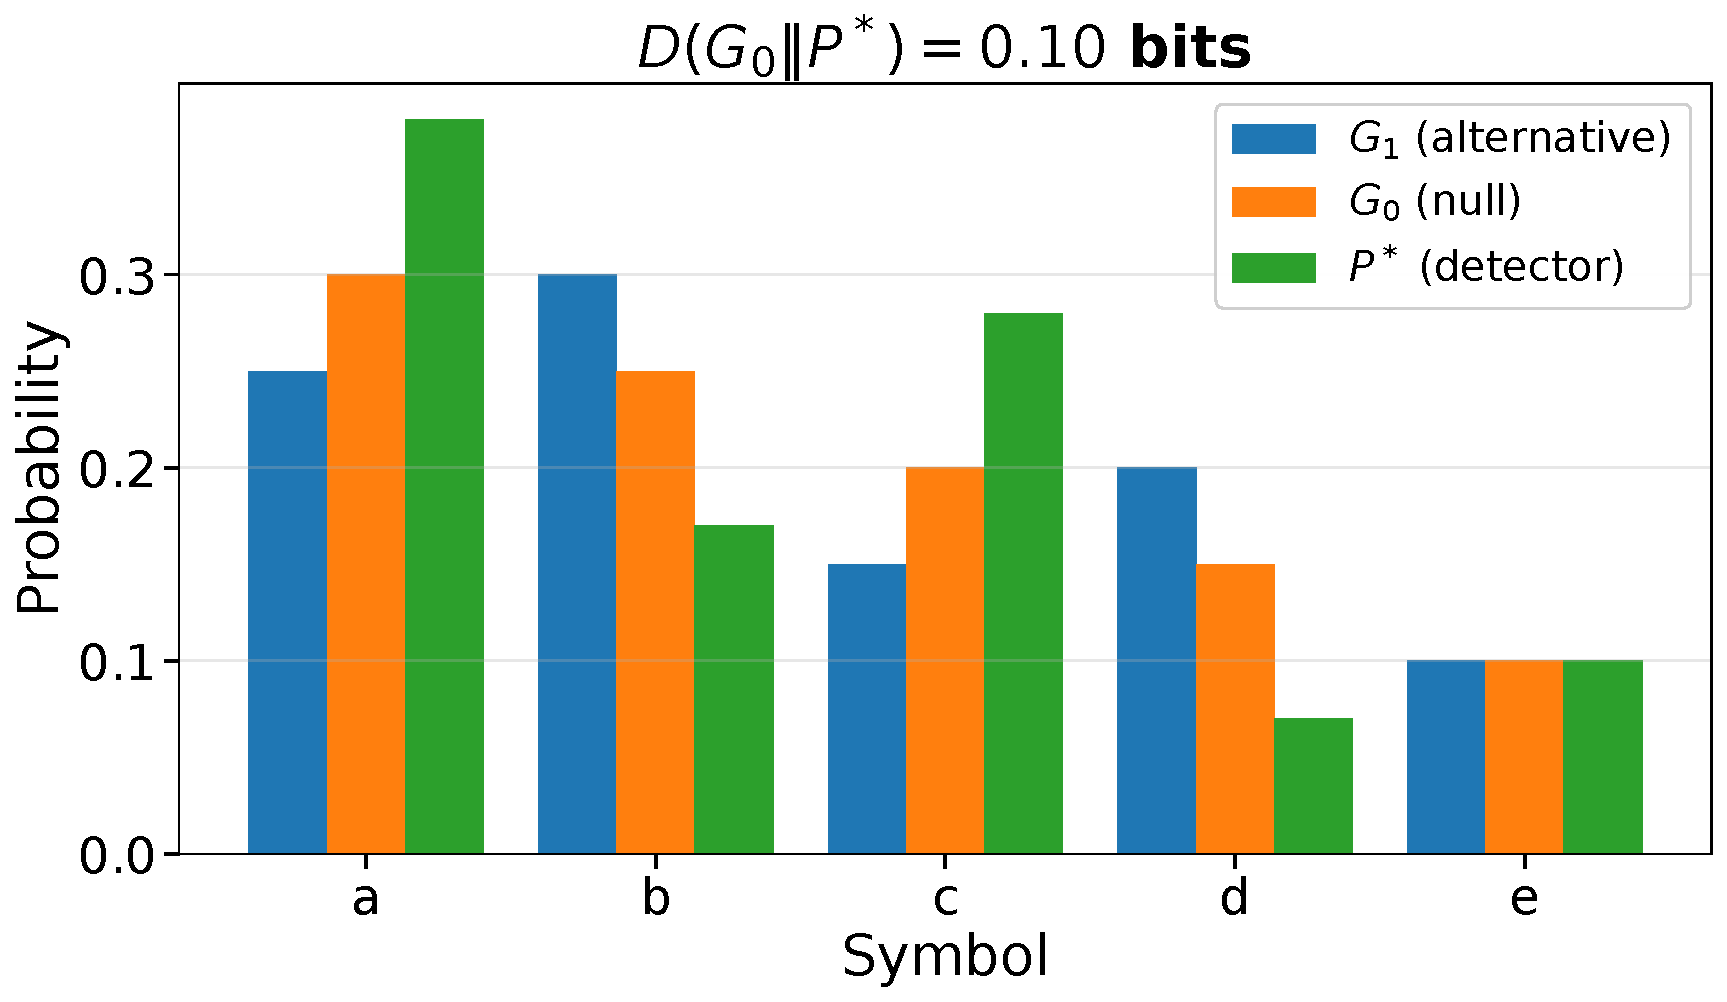
\includegraphics[width=0.80\linewidth, height=0.605\textheight, keepaspectratio]
    {figures/presentation/epsilon_ball_example.pdf}
\end{frame}

\note{
\textbf{Geometry of $P^*$ (Theorem 2).}
\begin{itemize}\small
  \item \textbf{The space is the probability simplex}: $G_0$, $G_1$, $P^*$ are
        each one point = a distribution over the alphabet. $G_1-G_0$ is the
        direction from $G_0$ toward $G_1$; $P^*$ steps the \emph{opposite} way
        (away from $G_1$) along a straight line.
  \item \textbf{Linear}, not geometric/exponential --- the small surprise of
        Thm~2. It subtracts mass from tokens where $G_1$ dominates, raising
        $-\log P$ there.
  \item $\epsilon$ = radius of the KL ball (the budget we choose); in the
        figure $\epsilon = 0.10$ bits --- that is exactly the
        ``$D(G_0\|P^*)=0.10$ bits'' label.
  \item $\gamma$ = step size in the formula; it is NOT free. Eq.~(10),
        $D(G_0\|P^*)=\epsilon$, pins $\gamma$ so $P^*$ lands exactly on the
        ball's boundary (constraint active, since $\Delta$ grows as we move
        away from $G_0$). So $\epsilon$ isn't written in eq.~(9): it enters
        through $\gamma$. Bigger $\epsilon\Rightarrow$ bigger
        $\gamma\Rightarrow P^*$ farther from $G_0$.
  \item \textbf{$\gamma\Leftrightarrow\epsilon$ relation:} no closed form in general
        (solve $\epsilon=-\sum_x G_0\log(1-\gamma\tfrac{G_1-G_0}{G_0})$,
        monotone in $\gamma$). Small-$\epsilon$:
        $\gamma\approx\sqrt{2\epsilon/\Dchi{G_1}{G_0}}$, i.e.
        $\gamma\propto\sqrt\epsilon$. This is the engine behind the
        Thm~3 gain $\sqrt{2\epsilon\,\Dchi{G_1}{G_0}}$.
        ($\epsilon$ in nats; $1/\ln2$ factor if in bits.)
\end{itemize}
}

% ------------------------------------------------------------------
% Frame 9 -- Composite alternatives and self-detection
% ------------------------------------------------------------------
\section{Composite Alternatives}
\begin{frame}[t]{Result 3: When Self-Detection is Locally Maximin-Optimal}
  \vspace{1.2em}
  \begin{columns}[c,onlytextwidth]
    \begin{column}{0.60\textwidth}
      {\small
      \textbf{Single \(G_1\):} move away from \(G_0\).\\[0.25em]
      \textbf{Family of alternatives \(\cG_1\):} optimize the worst case.}

      \[
        \bigDelta^*(\cG_1,G_0)=
        \sup_{P\in\cP_\epsilon(G_0)}\inf_{G\in\cG_1}\bigDelta(G,G_0;P)
      \]

      \vspace{0.5em}
      {\small \textbf{Modeling assumption:} LLM \(G_0\) can be viewed as a learned
      convex mixture of human-style sources:}

      \[
        G_0 \approx \sum_j \pi_j H_j
        \qquad \text{\footnotesize\(\pi_j\ge 0,\ \sum\nolimits_j \pi_j=1\)}
      \]
    \end{column}
    \hfill
    \begin{column}{0.39\textwidth}
      \centering
      \begin{tikzpicture}[scale=1.08]
        \fill[RUBlue] (0,0) circle (3pt)
             node[below=5pt, font=\normalsize]{$G_0$ {\footnotesize(LLM)}};
        \foreach \a in {0,20,...,340} {
          \pgfmathsetmacro{\r}{1.4+0.18*rand}
          \fill[red!50!black, opacity=0.55] (\a:\r) circle (1.8pt);
        }
        \draw[dashed, RUAccent, thick] (0,0) circle (1.6cm);
        \node[black, font=\small, align=center] at (0, -2.35)
             {alternative sources\\[-1pt] around \(G_0\)};
      \end{tikzpicture}
    \end{column}
  \end{columns}

  \vspace{0.15em}
  \begin{callout}[width=0.92\linewidth]
    {\small If alternatives \alert{isotropically surround} \(G_0\):}\\[2pt]
    {\Large \(\boldsymbol{P=G_0}\) is locally maximin optimal}
  \end{callout}
\end{frame}

% ------------------------------------------------------------------
% Frame 10 -- Empirical: normalized log-loss separation predicts AUC
% ------------------------------------------------------------------
\section{Evidence}
\begin{frame}[t]{Empirical Check: Normalized Separation Predicts AUC}
  \begin{columns}[c,onlytextwidth]
    \begin{column}{0.73\textwidth}
      \centering
      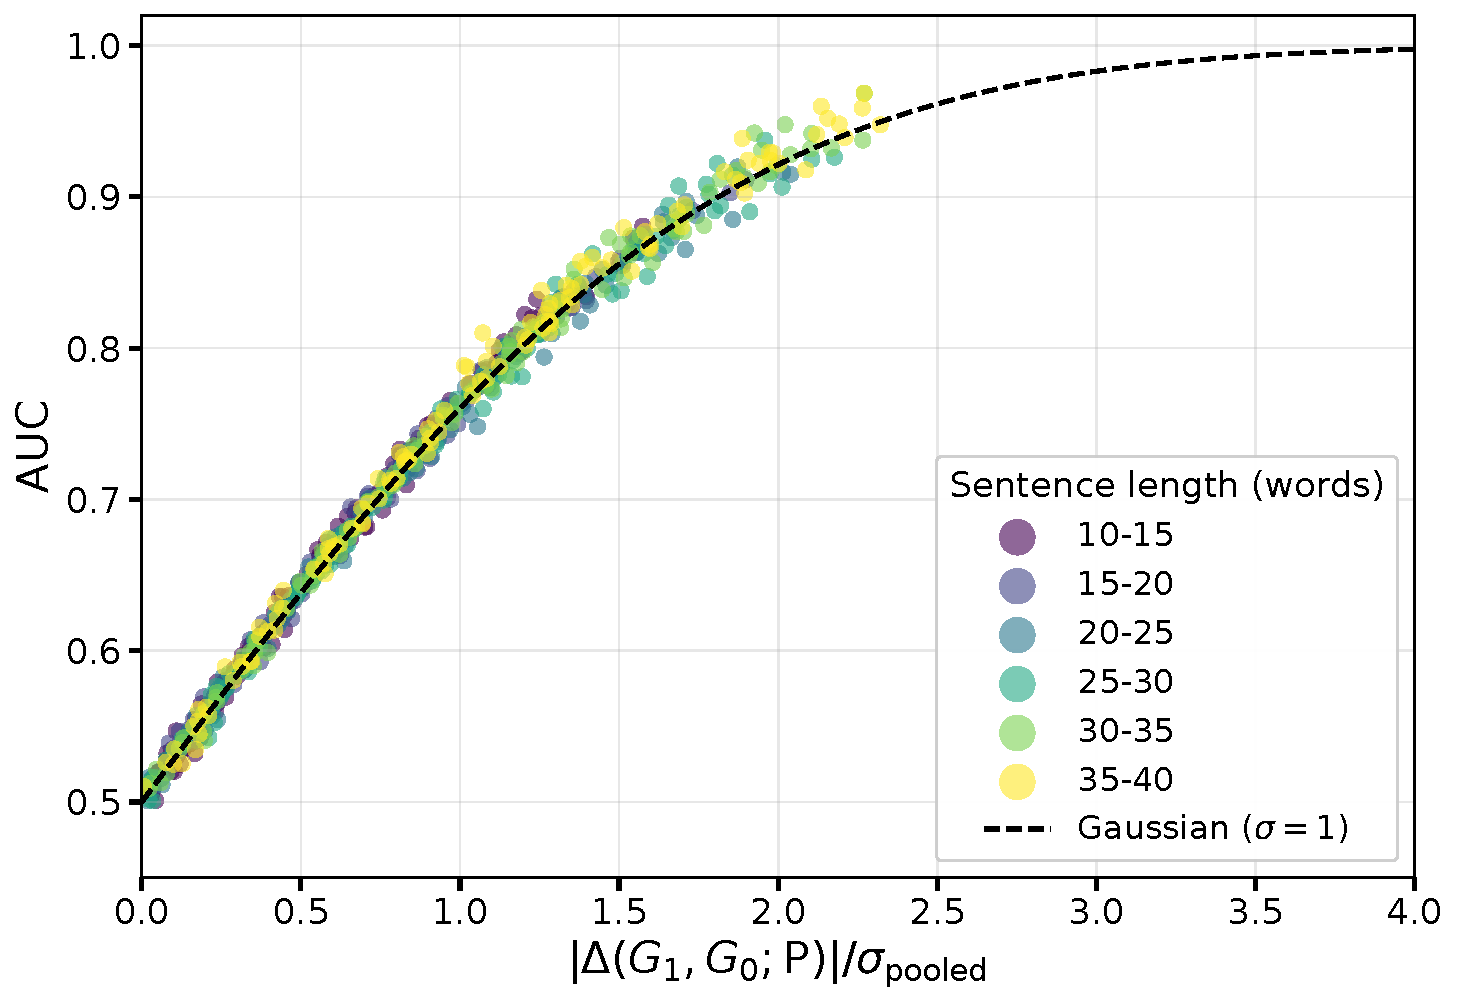
\includegraphics[width=\linewidth, height=0.625\textheight, keepaspectratio]
        {figures/presentation/auc_vs_delta_normalized_unified.pdf}
    \end{column}
    \hfill
    \begin{column}{0.25\textwidth}
      \small\textcolor{black!78}{%
      \(\displaystyle x:=\frac{|\hat\mu_1(P)-\hat\mu_0(P)|}{\hat\sigma_{\mathrm{pooled}}}\)\\[12pt]
      \(\mathrm{AUC}\approx\Phi(x/\sqrt{2})\)}
    \end{column}
  \end{columns}

  \vspace{0.3em}
  {\small \textbf{Experiment setup:} 275,000 sentences, 3 domains, 5 authors, 4 detector models}\\[2pt]
  {\small Empirical AUC follows the Gaussian curve:
  \alert{Pearson \(r=0.99\).}}\\[2pt]
  {\small\textcolor{RUBlue}{\textbf{Supports Result 1:}
  Gaussian-like log-loss behavior and stable variance.}}\\[2pt]
  {\footnotesize\textcolor{black!78}{Max/min standard-deviation ratio
  across detectors is \(1.2\)--\(1.5\times\).}}
\end{frame}

\note{
\textbf{VALIDATION, not a discovery.}
\begin{itemize}\small
  \item Don't pitch ``more separation $\to$ higher AUC'' as a finding ---
        obvious/monotone for any score.
  \item $\Phi(x/\sqrt2)$ = textbook binormal-AUC formula
        ($\mathrm{AUC}=\Pr(S_1>S_0)$ for two equal-variance Gaussians).
        We did NOT compute AUC with it: AUC is measured from the ROC
        (\texttt{roc\_auc\_score}); the curve is just overlaid. Parameter-free.
  \item Three claims tested: (1) $\Delta=D(G_1\|P)-D(G_0\|P)$ governs separation
        (Thm~1, not a priori obvious); (2) the unimodal, variance-stable
        Gaussian model (A1--A2) holds on real text; (3) the link is
        quantitative, not just directional.
  \item $r=0.99$ supports \textbf{A1--A2} (paper attributes Fig.~3 to A1--A2).
        \textbf{A3} ($\sigma$ independent of $P$) is checked \emph{separately}
        by the $1.2$--$1.5\times$ $\sigma$-ratio (Fig.~2). Single-$\sigma$ form
        assumes $\sigma_0\approx\sigma_1$; else
        $\Phi\!\big((\mu_1-\mu_0)/\sqrt{\sigma_0^2+\sigma_1^2}\big)$.
  \item Say: ``AUC measured from the ROC follows the parameter-free $\Phi(x/\sqrt2)$
        almost perfectly, so Thm~1's assumptions hold.'' Contribution = THEORY
        ($\Delta$ governs power; $P=G_0$ can be maximin); plot = credibility check.
\end{itemize}
}

% ------------------------------------------------------------------
% Frame 11 -- Human vs LLM evidence
% ------------------------------------------------------------------
\begin{frame}[t]{LLM vs.\ Human: Support for the Maximin Choice \(P=G_0\)}
  \centering
  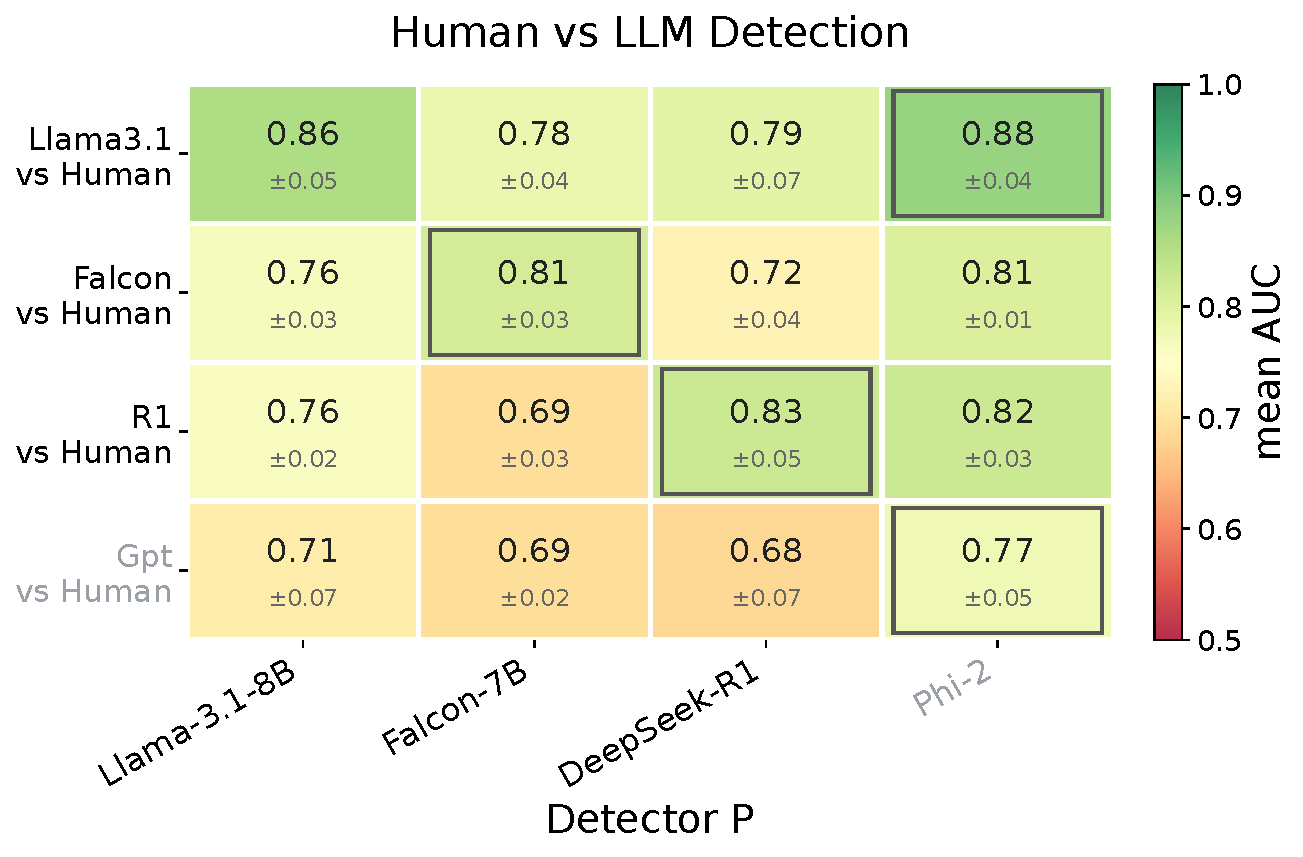
\includegraphics[width=0.98\linewidth, height=0.63\textheight, keepaspectratio]
    {figures/presentation/human_detection_heatmap_avg.pdf}

  \vfill
  \begin{columns}[c,onlytextwidth]
    \begin{column}{0.42\textwidth}
      \small\textbf{Matched detector \(P=G_0\):}
      \begin{itemize}
        \setlength\itemsep{0.1em}
        \item \alert{Best in 4/9} cases, second-best in 5/9
        \item Mean AUC \(\mathbf{0.831}\) vs.\ \(0.626\) for LLM-vs-LLM
      \end{itemize}
    \end{column}
    \hfill
    \begin{column}{0.55\textwidth}
      \begin{callout}[top=4pt,bottom=4pt,before skip=0pt,after skip=0pt,
          colframe=RUBlue!45, boxrule=0.5pt,
          borderline west={3pt}{0pt}{RUAccent}]
        \small Consistent with the maximin model if LLM \(G_0\) is surrounded
        by human sources.
      \end{callout}
    \end{column}
  \end{columns}
\end{frame}

% ------------------------------------------------------------------
% Frame 12 -- Contribution, not recap
% ------------------------------------------------------------------
\section{Takeaway}
\begin{frame}{Takeaway}
  \vfill
  \begin{enumerate}
    \setlength{\itemsep}{2.6em}
    \item When candidate-model likelihoods are unavailable,
          detect with a third model \(P\).

    \item The power-maximizing detector maximizes
          \(\bigDelta(G_1,G_0;P)=\Dkl{G_1}{P}-\Dkl{G_0}{P}\).

    \item For composite alternatives isotropically surrounding \(G_0\),
          self-detection is locally the maximin optimal choice.
  \end{enumerate}
  \vfill
\end{frame}

% ------------------------------------------------------------------
% Frame 13 -- Landing
% ------------------------------------------------------------------
{
\setbeamercolor{background canvas}{bg=RUBlue}
\setbeamercolor{normal text}{fg=white}
\usebeamercolor[fg]{normal text}
\hypersetup{urlcolor=white}
\begin{frame}[plain, c]
  \centering
  {\LARGE\textbf{Choose the detector. Maximize the gap.}}\\[1.8em]
  {\normalsize
    Adam Vinestock \quad\textbullet\quad
    \href{mailto:adam.vinestock@post.runi.ac.il}%
         {\texttt{adam.vinestock@post.runi.ac.il}}\\[3pt]
    Alon Kipnis \quad\textbullet\quad
    \href{mailto:alon.kipnis@runi.ac.il}%
         {\texttt{alon.kipnis@runi.ac.il}}
  }\\[1.4em]
  {\small Extended version \& proofs}\\[2pt]
  {\footnotesize\href{https://cs.idc.ac.il/~kipnis}%
                     {\texttt{cs.idc.ac.il/\~{}kipnis}}}
\end{frame}
}

% =================================================================
% BACKUP / APPENDIX
% =================================================================
\appendix
\metroset{numbering=none, progressbar=none}

% ------------------------------------------------------------------
% Backup B1 -- Theorem 3
% ------------------------------------------------------------------
\begin{frame}{How Sub-Optimal Is \(P=G_0\)?}
  Small-\(\epsilon\) expansion of the optimal gap:
  \[
    \bigDelta(G_1,G_0;P^*)
    =
    \Dkl{G_1}{G_0}
    +\sqrt{2\epsilon\,\Dchi{G_1}{G_0}}
    +O(\epsilon).
  \]

  \medskip
  \begin{callout}
    Deviating from \(G_0\) can raise the gap by
    \(\approx\sqrt{2\epsilon\,\Dchi{G_1}{G_0}}\),
    quantifying the sub-optimality of \(P=G_0\) against a
    \textbf{simple} alternative.
  \end{callout}

  \medskip
  \textbf{Where this comes from: the \(\gamma \Leftrightarrow \epsilon\) relation.}
  The constraint \(D(G_0\|P^*)=\epsilon\) fixes the step size \(\gamma\).
  It has no closed form in general, but for small \(\epsilon\)
  \[
    \epsilon \approx \tfrac{\gamma^2}{2}\,\Dchi{G_1}{G_0}
    \qquad\Longleftrightarrow\qquad
    \gamma \approx \sqrt{\tfrac{2\epsilon}{\Dchi{G_1}{G_0}}}
    \;\;(\gamma\propto\sqrt{\epsilon}),
  \]
  which substituted into the gap produces the
  \(\sqrt{2\epsilon\,\Dchi{G_1}{G_0}}\) term above.

  \medskip
  {\footnotesize Here
  \(\Dchi{G_1}{G_0}=\sum_x (G_1(x)-G_0(x))^2/G_0(x)\);
  \(\epsilon\) in nats (\(1/\ln2\) factor if measured in bits).}
\end{frame}

% ------------------------------------------------------------------
% Backup B2 -- Theorem 4
% ------------------------------------------------------------------
\begin{frame}{The Maximin Mechanism}
  For a composite family \(\cG_1\), the local maximin gap is set by
  a least-favorable prior \(\pi^*\):
  \[
    \bigDelta^*(\cG_1,G_0)
    =
    \mathbb{E}_{G\sim\pi^*}\!\left[\Dkl{G}{G_0}\right]
    +\sqrt{2\epsilon\,\Dchi{\bar G_{\pi^*}}{G_0}}
    +O(\epsilon),
  \]
  \[
    \bar G_{\pi^*}(x)=\mathbb{E}_{G\sim\pi^*}[G(x)].
  \]

  \begin{callout}
    If a non-convex alternative family isotropically surrounds \(G_0\),
    this mechanism yields Corollary 5.1: \(P=G_0\) is locally maximin.
  \end{callout}
\end{frame}

% ------------------------------------------------------------------
% Backup B2b -- Anisotropy index detail (definitions pushed off main slide 8)
% ------------------------------------------------------------------
\begin{frame}{Anisotropy Index and Isotropic Optimality}
  For a prior \(\pi^{\#}\) on \(\cG_1\) with \(G_0=\bar G_{\pi^{\#}}=\mathbb{E}_{G\sim\pi^{\#}}[G]\):
  \[
    \bar D_{\pi^{\#}}=\mathbb{E}_{G\sim\pi^{\#}}\Dkl{G}{G_0},
    \qquad
    r_{\pi^{\#}}=\sup_{G\in\operatorname{supp}(\pi^{\#})}
      \bigl|\Dkl{G}{G_0}-\bar D_{\pi^{\#}}\bigr|.
  \]
  \(r_{\pi^{\#}}=0\) iff all sources are equidistant from \(G_0\) in relative
  entropy (the mixture is isotropic); it grows with the unevenness of those
  distances.

  \medskip
  For any alternative \(G\in\cG_1\), the self-detector \(P=G_0\) obeys
  \[
    \bigDelta(G,G_0;G_0)=\Dkl{G}{G_0}
    \;\ge\;\bigDelta^*(\cG_1,G_0)-r_{\pi^{\#}}+O(\epsilon),
  \]
  so its worst-case sub-optimality is at most \(r_{\pi^{\#}}\). When
  \(r_{\pi^{\#}}=0\),
  \[
    \inf_{G\in\cG_1}\Dkl{G}{G_0}=\bigDelta^*(\cG_1,G_0)+O(\epsilon),
  \]
  i.e.\ \(P=G_0\) is locally maximin optimal.
\end{frame}

% ------------------------------------------------------------------
% Backup B3 -- Experimental setup
% ------------------------------------------------------------------
\begin{frame}{Experimental Setup}
  \begin{columns}[T,onlytextwidth]
    \begin{column}{0.48\textwidth}
      \textbf{Datasets} {\small(3 domains, matched topics)}
      \begin{itemize}
        \setlength\itemsep{0.25em}
        \item Wikipedia, News, Scientific abstracts
        \item \(\sim\!4{,}500\) docs, \(\sim\!275{,}000\) sentences
        \item Sentence length: 10--40 words
        \item Scored without preceding context
      \end{itemize}
    \end{column}
    \hfill
    \begin{column}{0.48\textwidth}
      \textbf{Authors / Detectors}
      \begin{itemize}
        \setlength\itemsep{0.25em}
        \item Authors: Llama-3.1, Falcon, GPT-3.5, DeepSeek-R1, Human
        \item Detectors \(P\): Llama-3.1, Falcon, Phi-2, DeepSeek-R1
        \item Some coincide \(\Rightarrow\) self-detection (\(P=G_0\))
      \end{itemize}
    \end{column}
  \end{columns}

  \vfill
  \begin{callout}
    GPT-3.5 model inaccessible for evaluation, so self-detection
    isn't possible.
  \end{callout}
\end{frame}

% ------------------------------------------------------------------
% Backup B4 -- Length confounding
% ------------------------------------------------------------------
\begin{frame}{Why Normalize?}
  \centering
  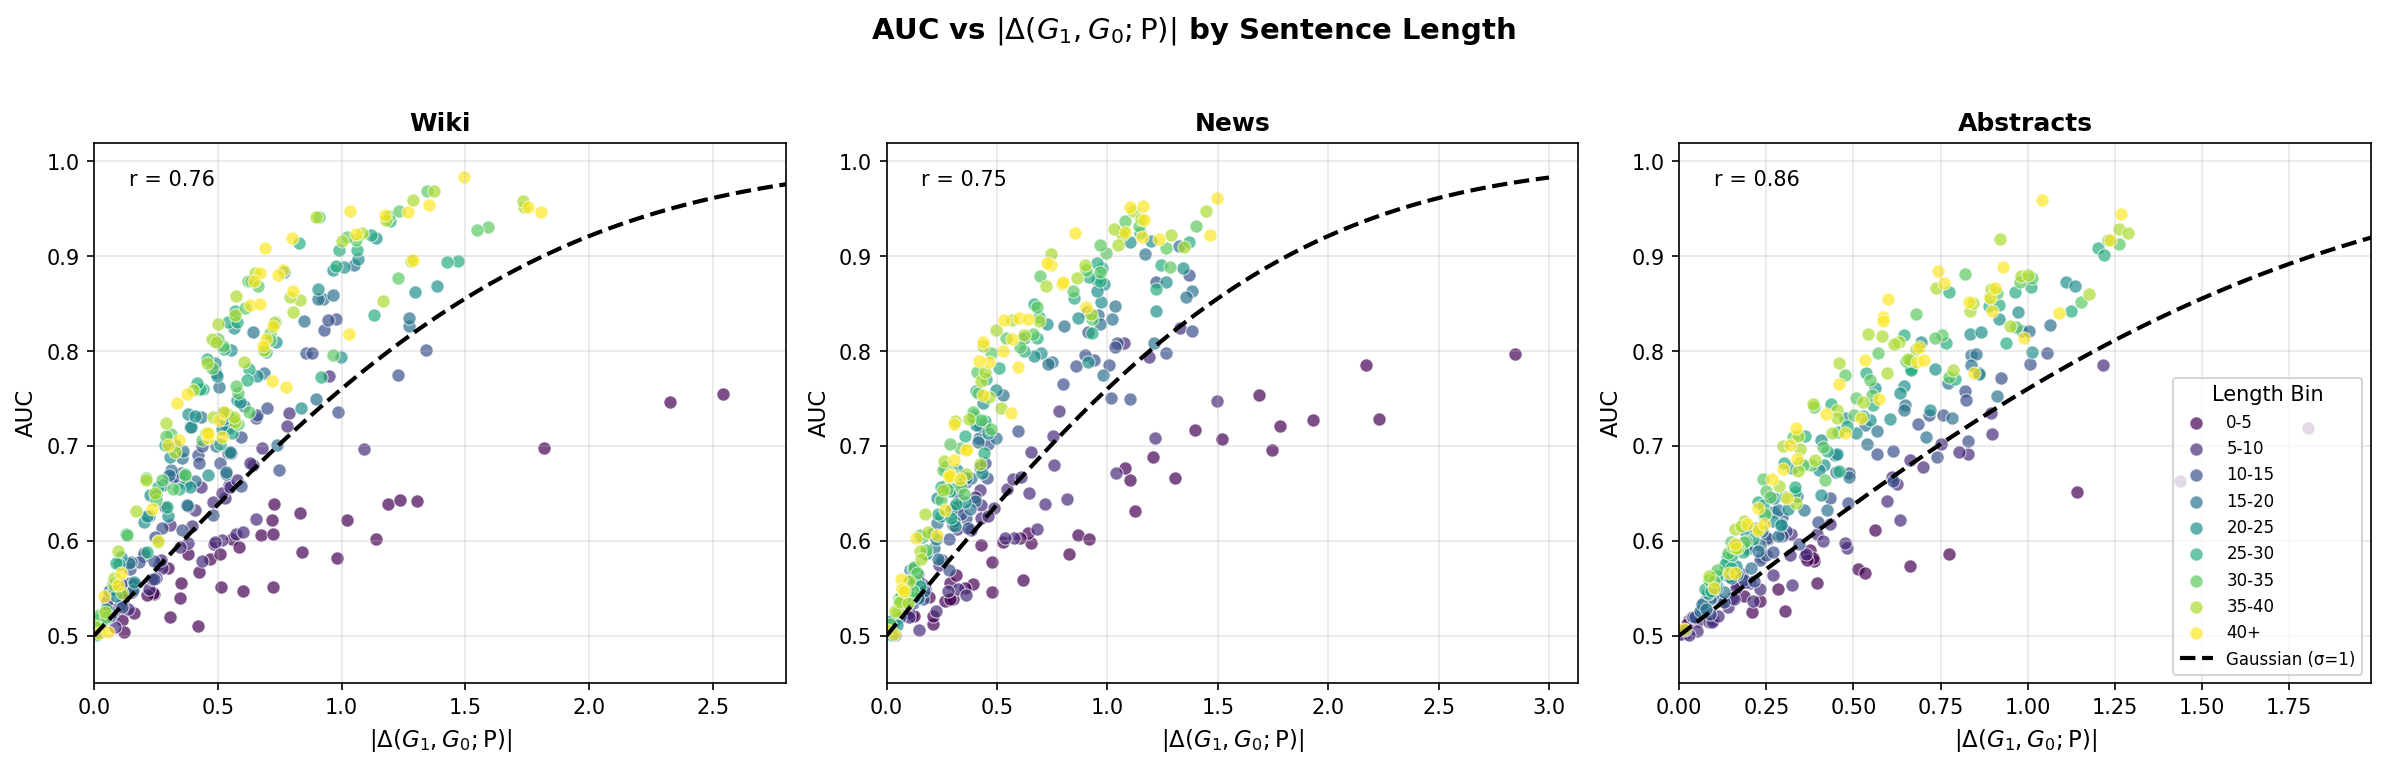
\includegraphics[width=0.95\linewidth, height=0.66\textheight, keepaspectratio]
    {figures/delta_auc_by_length.png}

  \vspace{0.3em}
  {\small Raw log-loss gaps are confounded by length. Dividing by
  \(\hat\sigma_{\mathrm{pooled}}\) collapses length bins onto the
  Gaussian AUC curve used in the main evidence slide.}
\end{frame}

% ------------------------------------------------------------------
% Backup B5 -- Variance stability
% ------------------------------------------------------------------
\begin{frame}{Variance Stability by Length}
  \centering
  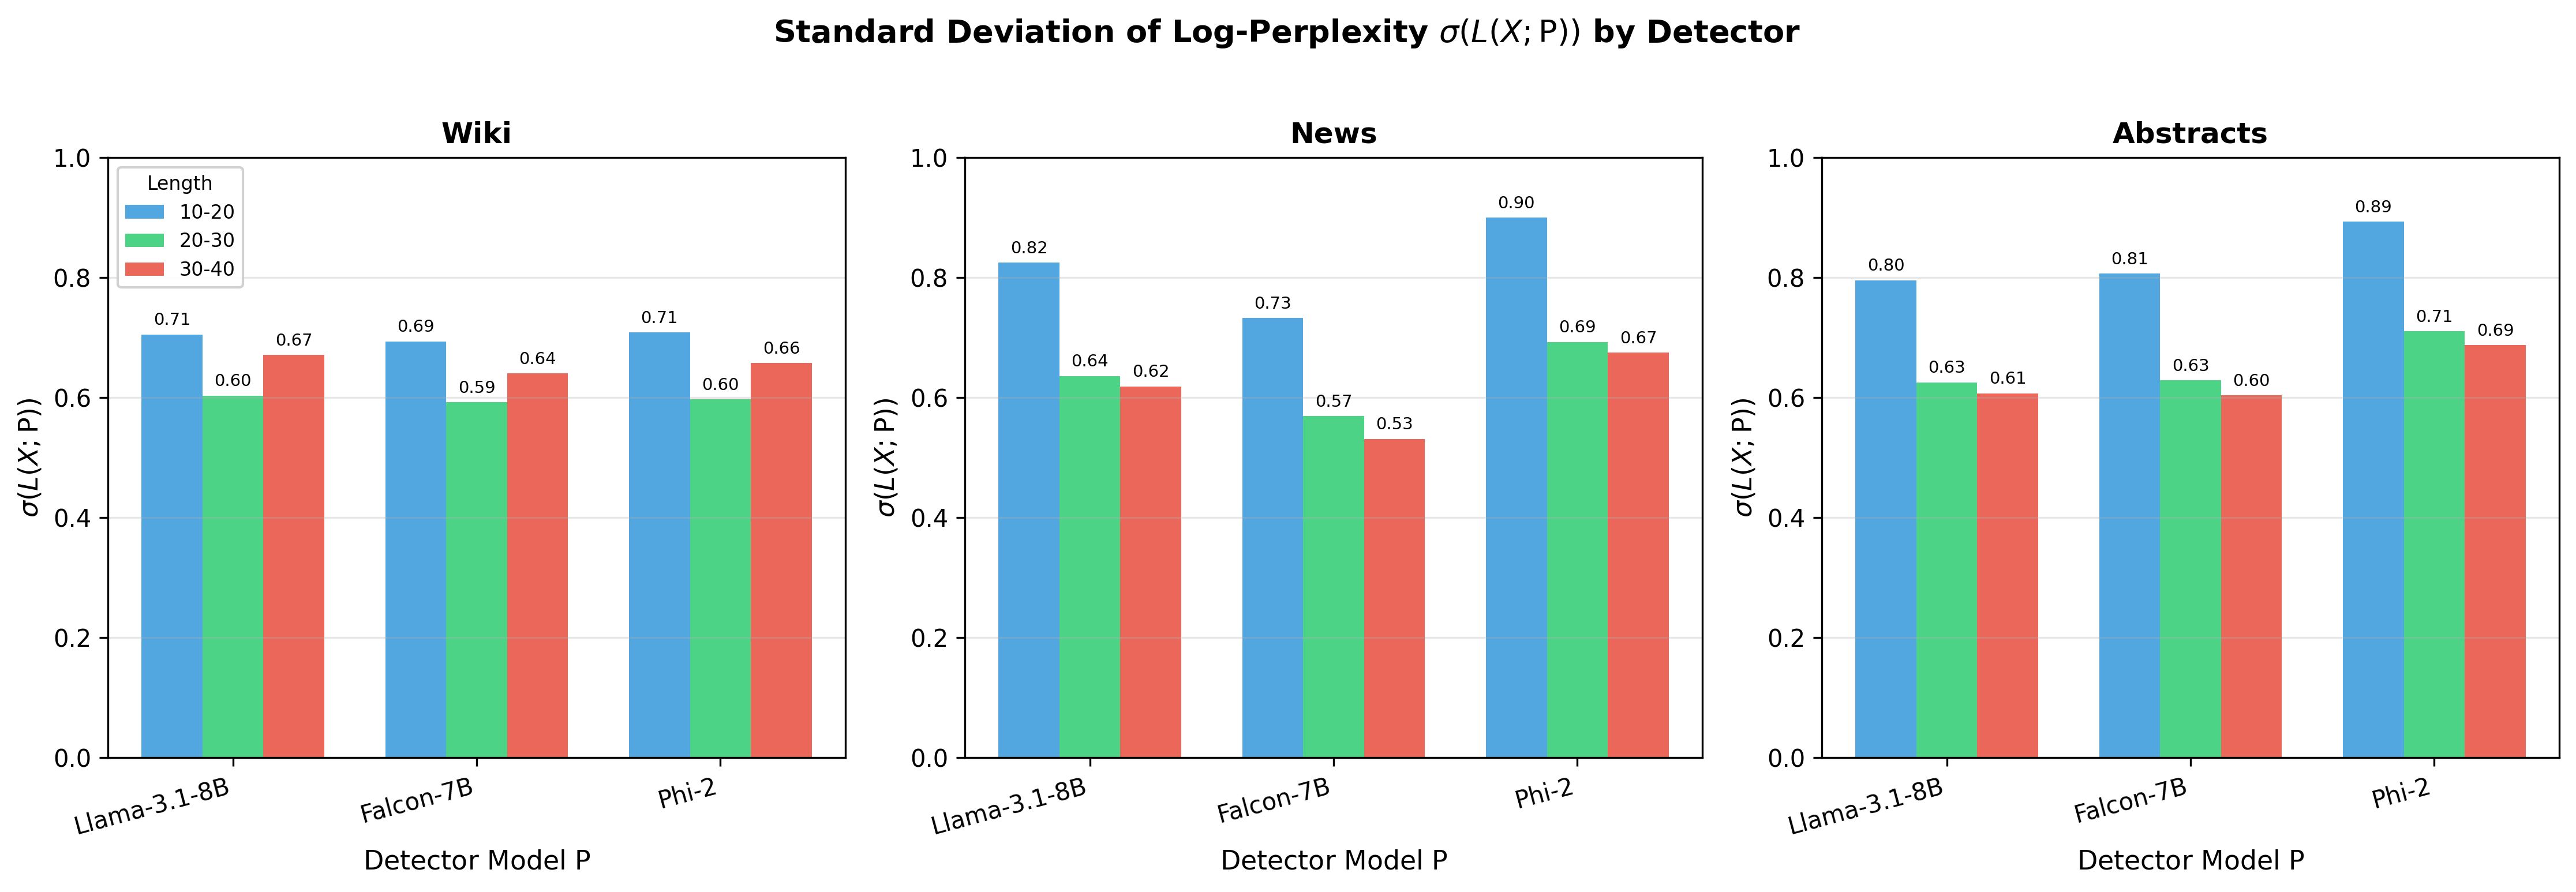
\includegraphics[width=\linewidth, height=0.62\textheight, keepaspectratio]
    {figures/sigma_vs_detector.png}

  \vspace{0.3em}
  {\small A3 view: standard deviation \(\sigma(L(X;P))\) by detector, split by
  sentence length. \emph{Within each length bin}, \(\sigma\) is nearly identical
  across Llama-3.1, Falcon, and Phi-2 (across-detector ratio \(\approx
  1.0\)--\(1.3\times\)), supporting A3; the larger spread within a dataset is
  driven by length, not by \(P\). DeepSeek-R1 is excluded as an outlier (its
  chat template inflates \(\sigma\)).}
\end{frame}

% ------------------------------------------------------------------
% Backup B6 -- Matched-detector counting
% ------------------------------------------------------------------
\begin{frame}{What ``Best in 4/9'' Means}
  \begin{itemize}
    \setlength\itemsep{0.55em}
    \item \textbf{The 9 cases:} 3 domains \(\times\) 3 matched LLM authors
          (Llama-3.1, Falcon, DeepSeek-R1).
    \item \textbf{GPT is excluded:} it has no corresponding open detector.
    \item \textbf{Phi-2 is detector-only:} it can win a heatmap cell, but
          is not part of the matched-detector count.
    \item \textbf{The claim:} among matched-detector cases,
          \(P=G_0\) is best in 4/9 and second-best in the remaining 5/9.
  \end{itemize}
\end{frame}

% ------------------------------------------------------------------
% Backup B7 -- AUC table
% ------------------------------------------------------------------
\begin{frame}{Matched-Detector AUC Numbers}
  \vfill
  \centering
  \textbf{AUC when detector matches source (\(P=G_0\))}

  \vspace{0.8em}
  \begin{tabular}{@{}lccc@{}}
    \toprule
    Dataset & Human vs.\ \(G_0\) & \(G_0\) vs.\ \(G_1\) & Gap \\
    \midrule
    Wiki      & \(0.853 \pm 0.006\) & \(0.659 \pm 0.065\) & \(+0.194\) \\
    News      & \(0.854 \pm 0.047\) & \(0.626 \pm 0.094\) & \(+0.229\) \\
    Abstracts & \(0.787 \pm 0.018\) & \(0.592 \pm 0.013\) & \(+0.195\) \\
    \midrule
    \textbf{Mean} & \(\mathbf{0.831}\) & \(\mathbf{0.626}\)
                  & \(\mathbf{+0.206}\) \\
    \bottomrule
  \end{tabular}

  \vspace{0.8em}
  {\small Human-vs-LLM self-detection is substantially easier than
  LLM-vs-LLM matched detection in this experiment.}
  \vfill
\end{frame}

% ------------------------------------------------------------------
% Backup B8--B10 -- Original (paper) versions of the updated plots
% ------------------------------------------------------------------
\begin{frame}{Backup: Original \(P^*\) Example (paper figure)}
  \centering
  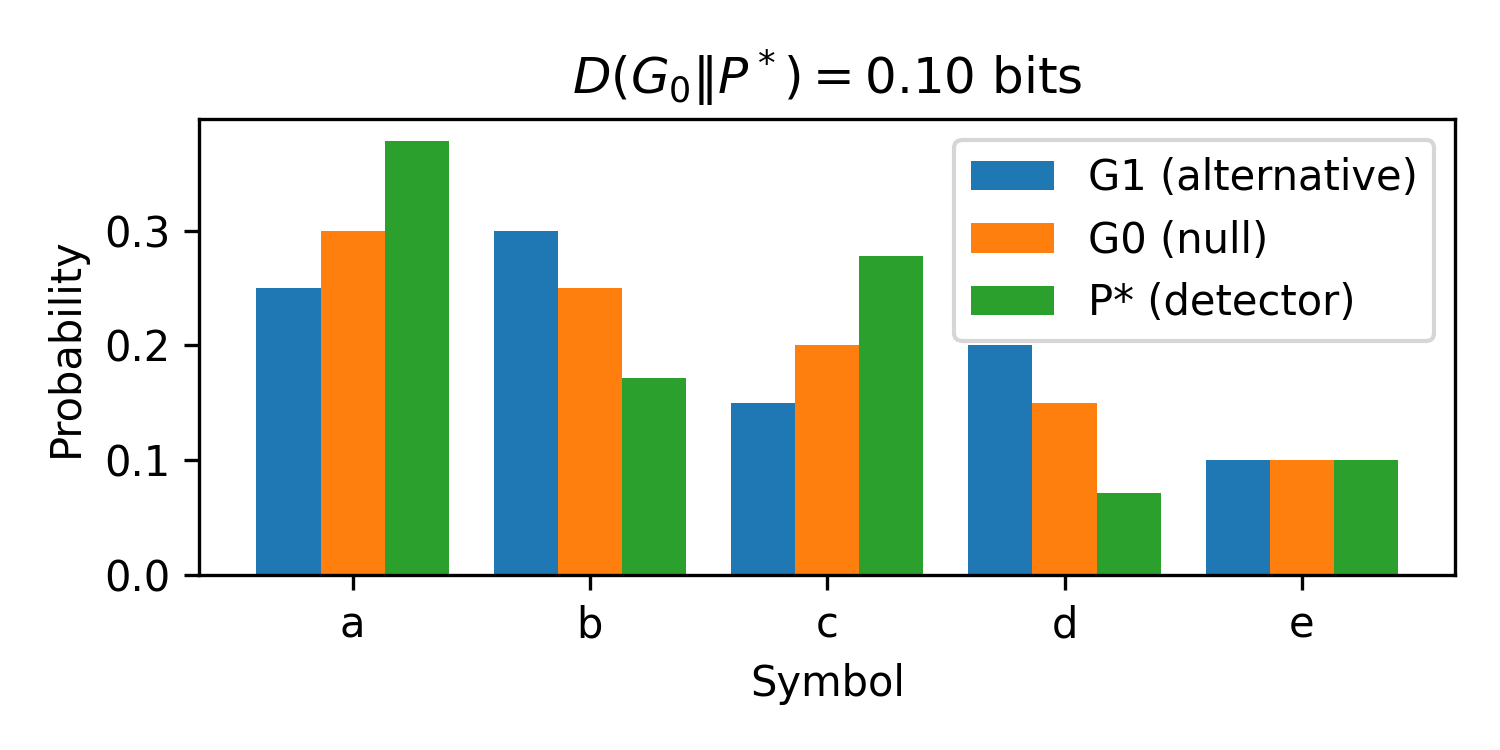
\includegraphics[width=0.92\linewidth, height=0.74\textheight, keepaspectratio]
    {figures/epsilon_ball_example.png}
\end{frame}

\begin{frame}{Backup: Original AUC vs Normalized Separation (paper figure)}
  \centering
  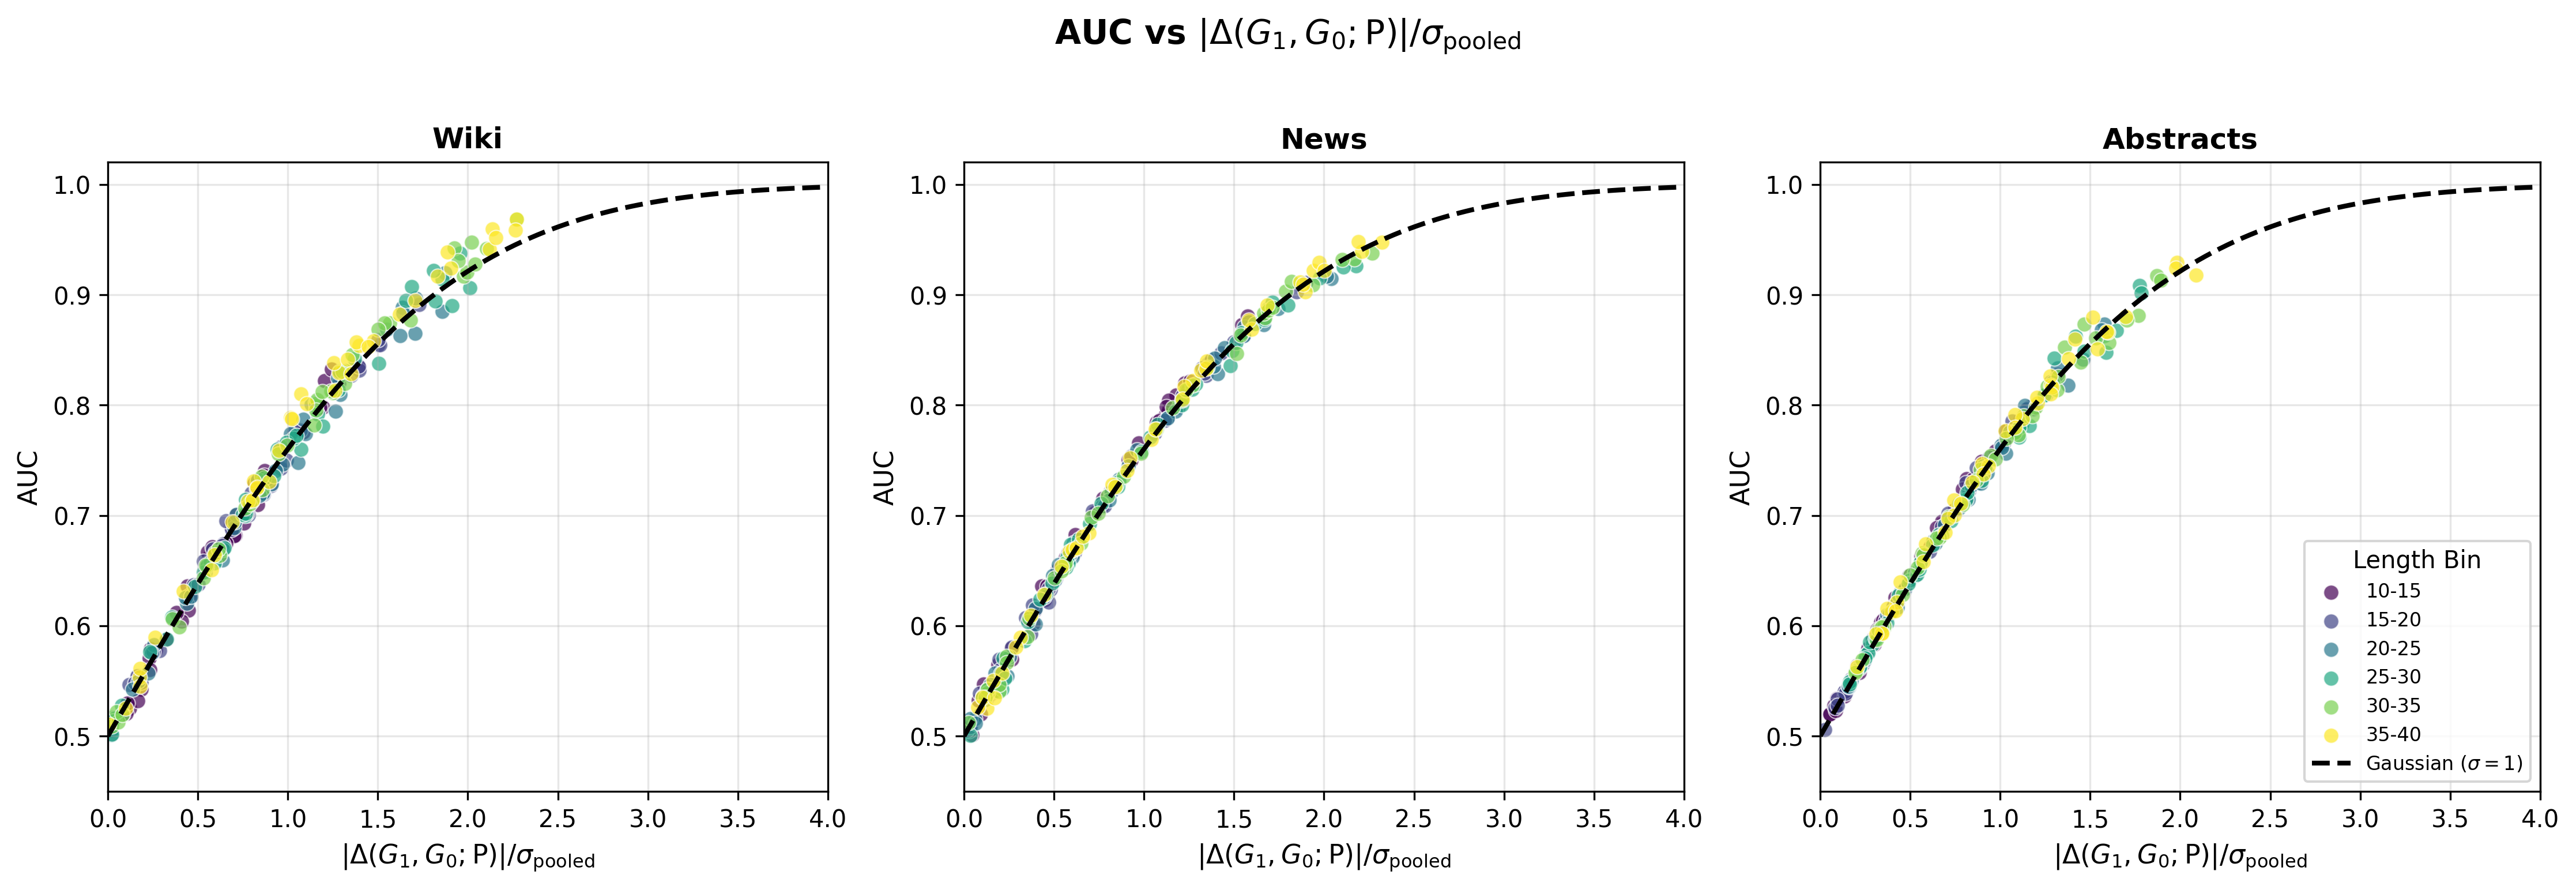
\includegraphics[width=0.96\linewidth, height=0.78\textheight, keepaspectratio]
    {figures/auc_vs_delta_normalized.png}
\end{frame}

\begin{frame}{Backup: Original Human-vs-LLM Heatmap (paper figure)}
  \centering
  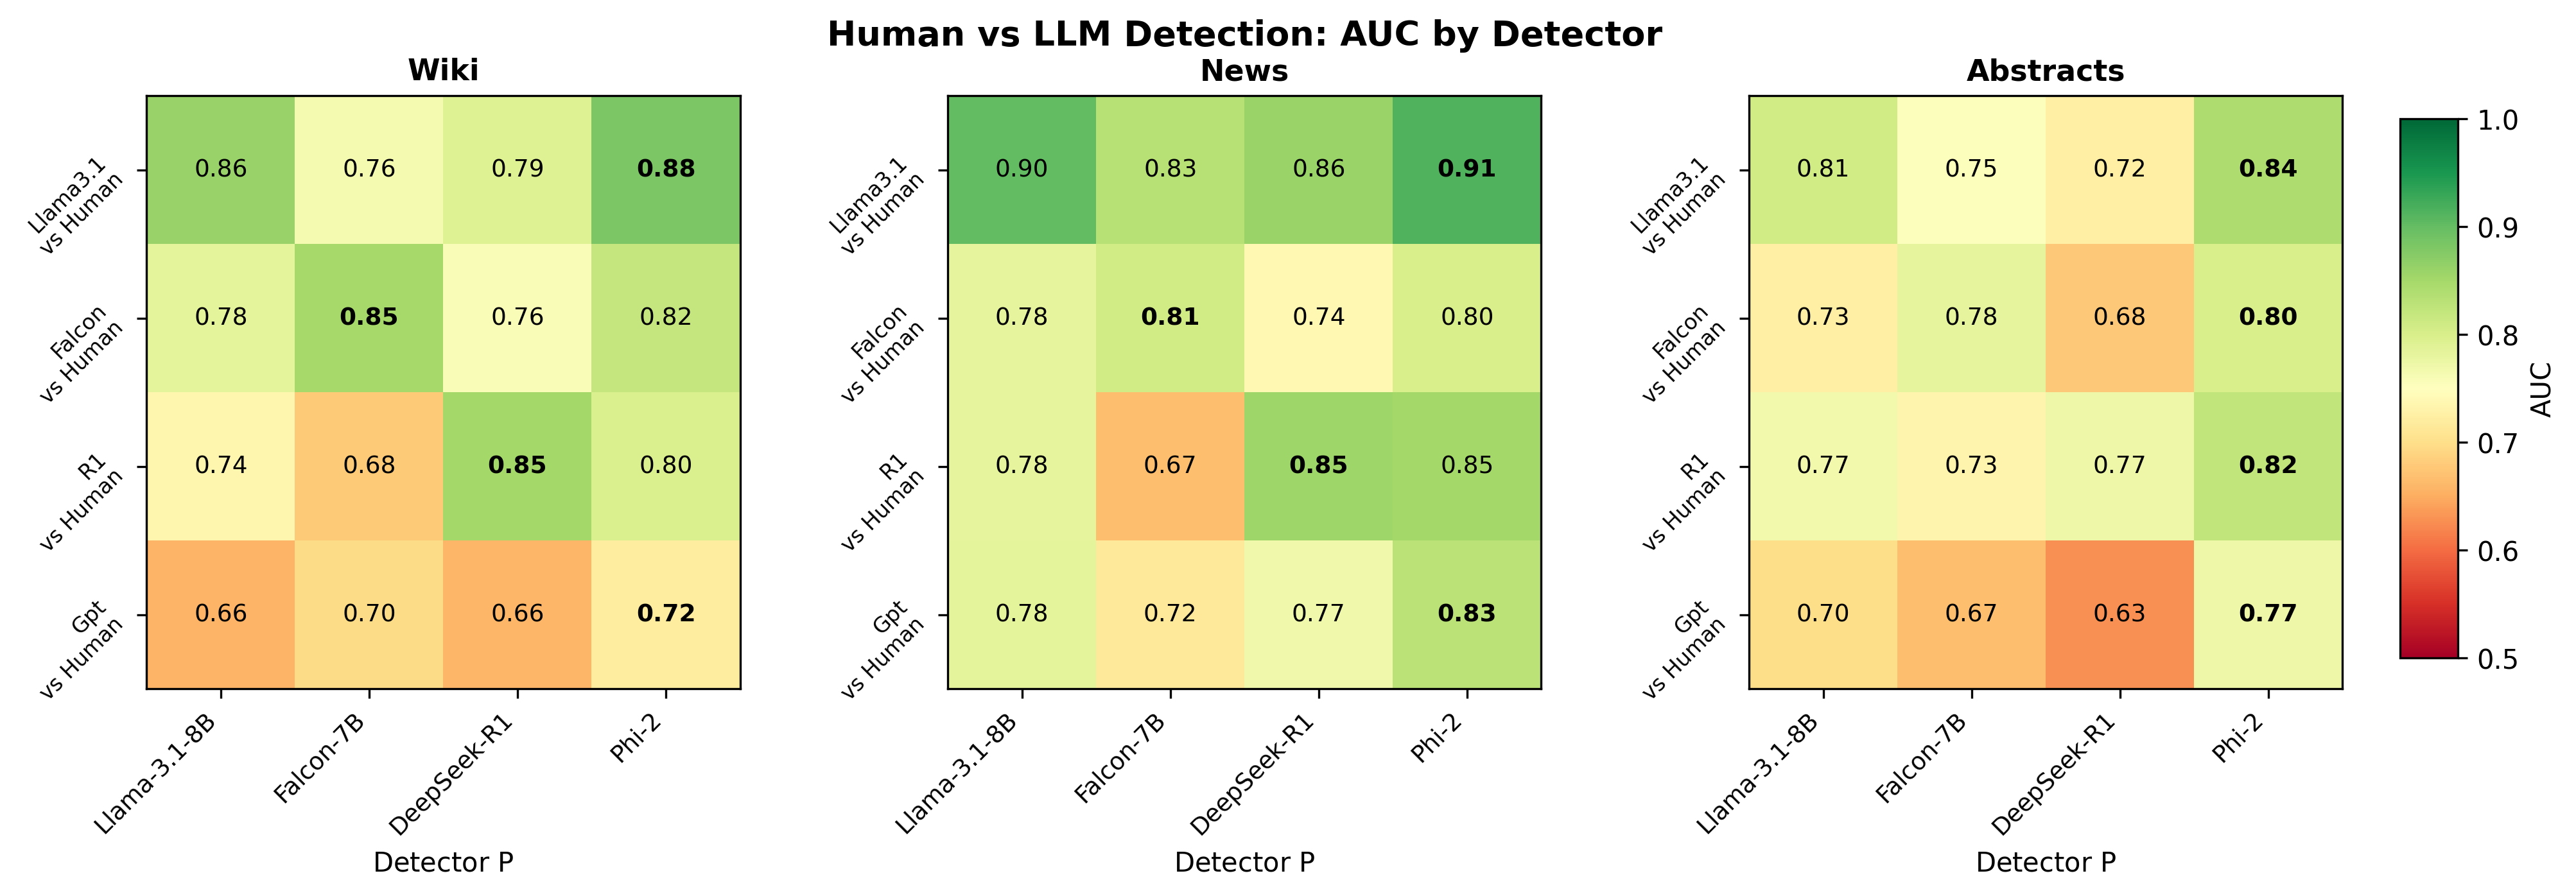
\includegraphics[width=0.96\linewidth, height=0.78\textheight, keepaspectratio]
    {figures/human_detection_heatmap.png}
\end{frame}

\end{document}
